% !TeX spellcheck = en-US
% !TeX encoding = utf8
% !TeX program = pdflatex
% !BIB program = biber
% -*- coding:utf-8 mod:LaTeX -*-


% vv  scroll down to line 200 for content  vv


\let\ifdeutsch\iffalse
\let\ifenglish\iftrue


% EN: This file is loaded before the \documentclass command in the main document

% EN: The following package allows \\ at the title page
%     For more information see https://github.com/latextemplates/scientific-thesis-cover/issues/4
\RequirePackage{kvoptions-patch}

\ifenglish
  \PassOptionsToClass{numbers=noenddot}{scrbook}
\else
  %()Aus scrguide.pdf - der Dokumentation von KOMA-Script)
  %Nach DUDEN steht in Gliederungen, in denen ausschließlich arabische Ziffern für die Nummerierung
  %verwendet werden, am Ende der Gliederungsnummern kein abschließender Punkt
  %(siehe [DUD96, R3]). Wird hingegen innerhalb der Gliederung auch mit römischen Zahlen
  %oder Groß- oder Kleinbuchstaben gearbeitet, so steht am Ende aller Gliederungsnummern ein
  %abschließender Punkt (siehe [DUD96, R4])
  \PassOptionsToClass{numbers=autoendperiod}{scrbook}
\fi

% Warns about outdated packages and missing caption declarations
% See https://www.ctan.org/pkg/nag
\RequirePackage[l2tabu, orthodox]{nag}

%DE: Neue deutsche Trennmuster
%    Siehe http://www.ctan.org/pkg/dehyph-exptl und http://projekte.dante.de/Trennmuster/WebHome
%    Nur für pdflatex, nicht für lualatex
\RequirePackage{ifluatex}
\ifluatex
  % do not load anything
\else
  \ifdeutsch
    \RequirePackage[ngerman=ngerman-x-latest]{hyphsubst}
  \fi
\fi

\documentclass[
  %
  %ngerman, %%% Add if you write in German.
  %
  % fontsize=11pt is the standard
  a4paper,  % Standard format - only KOMAScript uses paper=a4 - https://tex.stackexchange.com/a/61044/9075
  twoside,  % we are optimizing for both screen and two-side printing. So the page numbers will jump, but the content is configured to stay in the middle (by using the geometry package)
  bibliography=totoc,
  %               idxtotoc,   %Index ins Inhaltsverzeichnis
  %               liststotoc, %List of X ins Inhaltsverzeichnis, mit liststotocnumbered werden die Abbildungsverzeichnisse nummeriert
  headsepline,
  cleardoublepage=empty,
  parskip=half,
  %               draft    % um zu sehen, wo noch nachgebessert werden muss - wichtig, da Bindungskorrektur mit drin
  draft=false
]{scrbook}
% !TeX encoding = utf8
% -*- coding:utf-8 mod:LaTeX -*-

% EN: This file includes basic packages and sets options. The order of package
%     loading is important

% DE: In dieser Datei werden zuerst die benoetigten Pakete eingebunden und
%     danach diverse Optionen gesetzt. Achtung Reihenfolge ist entscheidend!


% EN: Styleguide:
% - English comments are prefixed with "EN", German comments are prefixed with "DE"
% - Prefixed headings define the language for the subsequent paragraphs
% - It is tried to organize packages in blocks. Bocks are separated by two empty lines.

% DE: Styleguide:
%
% Ein sehr kleiner Styleguide. Packages werden in Blöcken organisiert.
% Zwischen zwei Blöcken sind 2 Leerzeilen!


% EN: Enable copy and paste of text from the PDF
%     Only required for pdflatex. It "just works" in the case of lualatex.
%     mmap enables mathematical symbols, but does not work with the newtx font set
%     See: https://tex.stackexchange.com/a/64457/9075
%     Other solutions outlined at http://goemonx.blogspot.de/2012/01/pdflatex-ligaturen-und-copynpaste.html and http://tex.stackexchange.com/questions/4397/make-ligatures-in-linux-libertine-copyable-and-searchable
%     Trouble shooting outlined at https://tex.stackexchange.com/a/100618/9075

\ifluatex
\else
  \usepackage{cmap}
\fi


% EN: File encoding
% DE: Codierung
%     Wir sind im 21 Jahrhundert, utf-8 löst so viele Probleme.
%
% Mit UTF-8 funktionieren folgende Pakete nicht mehr. Bitte beachten!
%   * fancyvrb mit §
%   * easylist -> http://www.ctan.org/tex-archive/macros/latex/contrib/easylist/
\ifluatex
  % EN: See https://tex.stackexchange.com/a/158517/9075
  %     Not required, because of usage of fontspec package
  %\usepackage[utf8]{luainputenc}
\else
  \usepackage[utf8]{inputenc}
\fi


% DE: Parallelbetrieb tex4ht und pdflatex

\makeatletter
\@ifpackageloaded{tex4ht}{
  \def\iftex4ht{\iftrue}
}{
  \def\iftex4ht{\iffalse}
}
\makeatother


% EN: Mathematics
% DE: Mathematik
%
% DE: Viele Mathematik-Sachen. Siehe https://texdoc.net/pkg/amsmath
%
% EN: Options must be passed this way, otherwise it does not work with glossaries
% DE: fleqn (=Gleichungen linksbündig platzieren) funktioniert nicht direkt. Es muss noch ein Patch gemacht werden:
\PassOptionsToPackage{fleqn,leqno}{amsmath}
%
% DE: amsmath Muss nicht mehr geladen werden, da es von newtxmath automatisch geladen wird
% \usepackage{amsmath}


%% EN: Fonts
%% DE: Schriften
%%
%% !!! If you change the font, be sure that words such as "workflow" can
%% !!! still be copied from the PDF. If this is not the case, you have
%% !!! to use glyphtounicode. See comment at cmap package


% EN: Times Roman for all text
\ifluatex
  % source: Second proposed fix from the following answer: https://tex.stackexchange.com/a/394137
  \usepackage[no-math]{fontspec}
  \setmainfont{TeXGyreTermes-Regular}[
       BoldFont       = TeXGyreTermes-Bold ,
       ItalicFont     = TeXGyreTermes-Italic ,
       BoldItalicFont = TeXGyreTermes-BoldItalic,
       NFSSFamily     = ntxtlf]
  \setsansfont{TeX Gyre Heros Regular}[
       Scale=.9,
       BoldFont       = TeX Gyre Heros Bold,
       ItalicFont     = TeX Gyre Heros Italic,
       BoldItalicFont = TeX Gyre Heros BoldItalic]
  \setmonofont[StylisticSet={1,3},Scale=.9]{inconsolata}
  \RequirePackage{newtxmath}
\else
  \RequirePackage{newtxtext}
  \RequirePackage{newtxmath}
  % EN: looks good with times, but no equivalent for lualatex found,
  %     therefore replaced with inconsolata
  %\RequirePackage[zerostyle=b,scaled=.9]{newtxtt}
  \RequirePackage[varl,scaled=.9]{inconsolata}
\fi

% EN: Fallback font - if the subsequent font packages do not define a font (e.g., monospaced)
%     This is the modern package for "Computer Modern".
%     In case this gets activated, one has to switch from cmap package to glyphtounicode (in the case of pdflatex)
% DE: Fallback-Schriftart
%\usepackage[%
%    rm={oldstyle=false,proportional=true},%
%    sf={oldstyle=false,proportional=true},%
%    tt={oldstyle=false,proportional=true,variable=true},%
%    qt=false%
%]{cfr-lm}

% EN: Headings are typset in Helvetica (which is similar to Arial)
% DE: Schriftart fuer die Ueberschriften - ueberschreibt lmodern
%\usepackage[scaled=.95]{helvet}

% DE: Für Schreibschrift würde tun, muss aber nicht
%\usepackage{mathrsfs} %  \mathscr{ABC}

% EN: Font for the main text
% DE: Schriftart fuer den Fliesstext - ueberschreibt lmodern
%     Linux Libertine, siehe http://www.linuxlibertine.org/
%     Packageparamter [osf] = Minuskel-Ziffern
%     rm = libertine im Brottext, Linux Biolinum NICHT als serifenlose Schrift, sondern helvet (von oben) beibehalten
%\usepackage[rm]{libertine}

% EN: Alternative Font: Palantino. It is recommeded by Prof. Ludewig for German texts
% DE: Alternative Schriftart: Palantino, Packageparamter [osf] = Minuskel-Ziffern
%     Bitte nur in deutschen Texten
%\usepackage{mathpazo} %ftp://ftp.dante.de/tex-archive/fonts/mathpazo/ - Tipp aus DE-TEX-FAQ 8.2.1

% DE: Schriftart fuer Programmcode - ueberschreibt lmodern
%     Falls auskommentiert, wird die Standardschriftart lmodern genommen
%     Fuer schreibmaschinenartige Schluesselwoerter in den Listings - geht bei alten Installationen nicht, da einige Fontshapes (<>=) fehlen
%\usepackage[scaled=.92]{luximono}
%\usepackage{courier}
% DE: BeraMono als Typewriter-Schrift, Tipp von http://tex.stackexchange.com/a/71346/9075
%\usepackage[scaled=0.83]{beramono}

% EN: backticks (`) are rendered as such in verbatim environments.
%     See following links for details:
%     - https://tex.stackexchange.com/a/341057/9075
%     - https://tex.stackexchange.com/a/47451/9075
%     - https://tex.stackexchange.com/a/166791/9075
\usepackage{upquote}

% DE: Symbole
%
%\usepackage[geometry]{ifsym} % \BigSquare
%\usepackage{mathabx}
%\usepackage{stmaryrd} %fuer \ovee, \owedge, \otimes
%\usepackage{marvosym} %fuer \Writinghand %patched to not redefine \Rightarrow
%\usepackage{mathrsfs} %mittels \mathscr{} schoenen geschwungenen Buchstaben erzeugen
%\usepackage{calrsfs} %\mathcal{} ein bisserl dickeren buchstaben erzeugen - sieht net so gut aus.
%durch mathpazo ist das schon definiert

%
%\usepackage{amssymb}

% EN: For \texttrademark{}
\usepackage{textcomp}

% EN: name-clashes von marvosym und mathabx vermeiden:
\def\delsym#1{%
  %  \expandafter\let\expandafter\origsym\expandafter=\csname#1\endcsname
  %  \expandafter\let\csname orig#1\endcsname=\origsym
  \expandafter\let\csname#1\endcsname=\relax
}

%\usepackage{pifont}
%\usepackage{bbding}
%\delsym{Asterisk}
%\delsym{Sun}\delsym{Mercury}\delsym{Venus}\delsym{Earth}\delsym{Mars}
%\delsym{Jupiter}\delsym{Saturn}\delsym{Uranus}\delsym{Neptune}
%\delsym{Pluto}\delsym{Aries}\delsym{Taurus}\delsym{Gemini}
%\delsym{Rightarrow}
%\usepackage{mathabx} - Ueberschreibt leider zu viel - und die \le-Zeichen usw. sehen nicht gut aus!


% EN: Modern font encoding
%     Has to be loaded AFTER any font packages. See https://tex.stackexchange.com/a/2869/9075.
\ifluatex
\else
  \usepackage[T1]{fontenc}
\fi
%


% EN: Character protrusion and font expansion. See http://www.ctan.org/tex-archive/macros/latex/contrib/microtype/
% DE: Optischer Randausgleich und Grauwertkorrektur

\usepackage[
  babel=true, % EN: Enable language-specific kerning. Take language-settings from the languge of the current document (see Section 6 of microtype.pdf)
  expansion=alltext,
  protrusion=alltext-nott, % EN: Ensure that at listings, there is no change at the margin of the listing
  final % EN: Always enable microtype, even if in draft mode. This helps finding bad boxes quickly.
        %     In the standard configuration, this template is always in the final mode, so this option only makes a difference if "pros" use the draft mode
]{microtype}


% EN: \texttt{test -- test} keeps the "--" as "--" (and does not convert it to an en dash)
\DisableLigatures{encoding = T1, family = tt* }

% DE: fuer microtype
% DE: tracking=true muss als Parameter des microtype-packages mitgegeben werden
% DE: Deaktiviert, da dies bei Algorithmen seltsam aussieht

%\DeclareMicrotypeSet*[tracking]{my}{ font = */*/*/sc/* }%
%\SetTracking{ encoding = *, shape = sc }{ 45 }
% DE: Hier wird festgelegt,
%     dass alle Passagen in Kapitälchen automatisch leicht
%     gesperrt werden.
%     Quelle: http://homepage.ruhr-uni-bochum.de/Georg.Verweyen/pakete.html
%    Deaktiviert, da sonst "BPEL", "BPMN" usw. wirklich komisch aussehen.
%     Macht wohl nur bei geisteswissenschaftlichen Arbeiten Sinn.


% EN: amsmath teaks


% EN: Fixes bugs in AMS math
%     Corrently conflicts with unicode-math
% \usepackage{mathtools}

%\numberwithin{equation}{section}
%\renewcommand{\theequation}{\thesection.\Roman{equation}}

% EN: work-around ams-math problem with align and 9 -> 10. Does not work with glossaries, No visual changes.
%\addtolength\mathindent{1em}


% EN: For theorems, replacement for amsthm
\usepackage[amsmath,hyperref]{ntheorem}
\theorempreskipamount 2ex plus1ex minus0.5ex
\theorempostskipamount 2ex plus1ex minus0.5ex
\theoremstyle{break}
\newtheorem{definition}{Definition}[section]


% CTAN: https://ctan.org/pkg/lccaps
% Doc: http://texdoc.net/pkg/lccaps
%
% Required for DE/EN \initialism
\usepackage{lccaps}


% EN: Defintion of colors. Argument "hyperref" is not used as we do not want to change border colors of links: Links are not colored anymore.
% DE: Farbdefinitionen
\usepackage[dvipsnames]{xcolor}


% EN: Required for custom acronyms/glossaries style.
%     Left aligned Columns in tables with fixed width.
%     See http://tex.stackexchange.com/questions/91566/syntax-similar-to-centering-for-right-and-left
\usepackage{ragged2e}


% DE: Wichtig, ansonsten erscheint "No room for a new \write"
\usepackage{scrwfile}


% EN: Support for language-specific hyphenation
% DE: Neue deutsche Rechtschreibung und Literatur statt "Literature"
%     Die folgende Einstellung ist der Nachfolger von ngerman.sty
\ifdeutsch
  % DE: letzte Sprache ist default, Einbindung von "american" ermöglicht \begin{otherlanguage}{amercian}...\end{otherlanguage} oder \foreignlanguage{american}{Text in American}
  %     Siehe auch http://tex.stackexchange.com/a/50638/9075
  \usepackage[american,main=ngerman]{babel}
  % Ein "abstract" ist eine "Kurzfassung", keine "Zusammenfassung"
  \addto\captionsngerman{%
    \renewcommand\abstractname{Kurzfassung}%
  }
  \ifluatex
    % EN: conditionally disable ligatures. See https://github.com/latextemplates/scientific-thesis-template/issues/54
    %     for a discussion
    \usepackage[ngerman]{selnolig}
  \fi
\else
  % EN: Set English as language and allow to write hyphenated"=words
  %     `american`, `english` and `USenglish` are synonyms for babel package (according to https://tex.stackexchange.com/questions/12775/babel-english-american-usenglish).
  %      "english" has to go last to set it as default language
  \usepackage[english]{babel}
  % EN: Hint by http://tex.stackexchange.com/a/321066/9075 -> enable "= as dashes
  \addto\extrasenglish{\languageshorthands{ngerman}\useshorthands{"}}
  \ifluatex
    % EN: conditionally disable ligatures. See https://github.com/latextemplates/scientific-thesis-template/issues/54
    %     for a discussion
    \usepackage[english]{selnolig}
  \fi
\fi
%


% EN: For easy quotations: \enquote{text}
%     This package is very smart when nesting is applied, otherwise textcmds (see below) provides a shorter command
%     Note that this package results in a warning when it is loaded before minted (actually fvextra).
% DE: Anführungszeichen
%     Zitate in \enquote{...} setzen, dann werden automatisch die richtigen Anführungszeichen verwendet.
%     Dieses package erzeugt eine Warnung, wenn es vor minted (genauer fvextra) geladen wird.
\usepackage{csquotes}


% EN: For even easier quotations: \qq{text}.
%     Is not smart in the case of nesting, but good enough for the most cases
\usepackage{textcmds}
\ifdeutsch
  % EN: German quotes are different. So do not use the English quotes, but the ones provided by the csquotes package.
  \renewcommand{\qq}[1]{\enquote{#1}}
\fi


% EN: extended enumarations
% DE: erweitertes Enumerate
\usepackage{paralist}


% DE: Gestaltung der Kopf- und Fußteilen

\usepackage[automark]{scrlayer-scrpage}

\automark[section]{chapter}
\setkomafont{pageheadfoot}{\normalfont\sffamily}
\setkomafont{pagenumber}{\normalfont\sffamily}

% DE: funktioniert nicht: Alle Linien sind hier weg
%\setheadsepline[.4pt]{.4pt}


% DE: Intelligentes Leerzeichen um hinter Abkürzungen die richtigen Abstände zu erhalten, auch leere.
%     Siehe commands.tex \gq{}
\usepackage{xspace}
% DE: Macht \xspace und \enquote kompatibel
\makeatletter
\xspaceaddexceptions{\grqq \grq \csq@qclose@i \} }
\makeatother


\newcommand{\eg}{e.\,g.,\ }
\newcommand{\ie}{i.\,e.,\ }


% EN: introduce \powerset - hint by http://matheplanet.com/matheplanet/nuke/html/viewtopic.php?topic=136492&post_id=997377
\DeclareFontFamily{U}{MnSymbolC}{}
\DeclareSymbolFont{MnSyC}{U}{MnSymbolC}{m}{n}
\DeclareFontShape{U}{MnSymbolC}{m}{n}{
  <-6>    MnSymbolC5
  <6-7>   MnSymbolC6
  <7-8>   MnSymbolC7
  <8-9>   MnSymbolC8
  <9-10>  MnSymbolC9
  <10-12> MnSymbolC10
  <12->   MnSymbolC12%
}{}
\DeclareMathSymbol{\powerset}{\mathord}{MnSyC}{180}


% EN: Package for the appendix
% DE: Anhang
\usepackage{appendix}
%[toc,page,title,header]
%


% EN: Graphics
% DE: Grafikeinbindungen
%
% EN: The parameter "pdftex" is not required
\usepackage{graphicx}
\graphicspath{{\getgraphicspath}}
\newcommand{\getgraphicspath}{graphics/}

% EN: Enables inclusion of SVG graphics
\usepackage{svg}

% EN: Enable typesetting values with SI units.
%\ifdeutsch
%  \usepackage[mode=text,group-four-digits]{siunitx}
%  \sisetup{locale=DE}
%\else
%  \usepackage[mode=text,group-four-digits,group-separator={,}]{siunitx}
%  \sisetup{locale=US}
%\fi


% EN: Extensions for tables
% DE: Tabellenerweiterungen
\usepackage{array} %increases tex's buffer size and enables ``>'' in tablespecs
\usepackage{longtable}
\usepackage{dcolumn} %Aligning numbers by decimal points in table columns
\ifdeutsch
  \newcolumntype{d}[1]{D{.}{,}{#1}}
\else
  \newcolumntype{d}[1]{D{.}{.}{#1}}
\fi
\setlength{\extrarowheight}{1pt}


% DE: Eine Zelle, die sich über mehrere Zeilen erstreckt.
%     Siehe Beispieltabelle in Kapitel 2
\usepackage{multirow}


% DE: Fuer Tabellen mit Variablen Spaltenbreiten
%\usepackage{tabularx}
%\usepackage{tabulary}


% EN: Links behave as they should. Enables "\url{...}" for URL typesettings.
%     Allow URL breaks also at a hyphen, even though it might be confusing: Is the "-" part of the address or just a hyphen?
%     See https://tex.stackexchange.com/a/3034/9075.
% DE: Links verhalten sich so, wie sie sollen
%     Zeilenumbrüche bei URLs auch bei Bindestrichen erlauben, auch wenn es verwirrend sein könnte: Gehört der Bindestrich zur URL oder ist es ein Trennstrich?
%     Siehe https://tex.stackexchange.com/a/3034/9075.
\usepackage[hyphens]{url}
%
%  EN: When activated, use text font as url font, not the monospaced one.
%      For all options see https://tex.stackexchange.com/a/261435/9075.
% \urlstyle{same}
%
% EN: Hint by http://tex.stackexchange.com/a/10419/9075.
\makeatletter
\g@addto@macro{\UrlBreaks}{\UrlOrds}
\makeatother


% DE: Index über Begriffe, Abkürzungen
%\usepackage{makeidx} makeidx ist out -> http://xindy.sf.net verwenden


% DE: lustiger Hack fuer das Abkuerzungsverzeichnis
%     nach latex durchlauf folgendes ausfuehren
%     makeindex ausarbeitung.nlo -s nomencl.ist -o ausarbeitung.nls
%     danach nochmal latex
%\usepackage{nomencl}
%    \let\abk\nomenclature %Deutsche Ueberschrift setzen
%          \renewcommand{\nomname}{List of Abbreviations}
%        %Punkte zw. Abkuerzung und Erklaerung
%          \setlength{\nomlabelwidth}{.2\hsize}
%          \renewcommand{\nomlabel}[1]{#1 \dotfill}
%        %Zeilenabstaende verkleinern
%          \setlength{\nomitemsep}{-\parsep}
%    \makenomenclature


% EN: Logic for TeX - enables if-then-else in commands
% DE: Logik für TeX
%     FÜr if-then-else @ commands.tex
\usepackage{ifthen}


% EN: Code Listings
% DE: Listings
\usepackage{listings}
\lstset{language=XML,
  showstringspaces=false,
  extendedchars=true,
  basicstyle=\footnotesize\ttfamily,
  commentstyle=\slshape,
  % DE: Original: \rmfamily, damit werden die Strings im Quellcode hervorgehoben. Zusaetzlich evtl.: \scshape oder \rmfamily durch \ttfamily ersetzen. Dann sieht's aus, wie bei fancyvrb
  stringstyle=\ttfamily,
  breaklines=true,
  breakatwhitespace=true,
  % EN: alternative: fixed
  columns=flexible,
  numbers=left,
  numberstyle=\tiny,
  basewidth=.5em,
  xleftmargin=.5cm,
  % aboveskip=0mm, %DE: deaktivieren, falls man lstlistings direkt als floating object benutzt (\begin{lstlisting}[float,...])
  % belowskip=0mm, %DE: deaktivieren, falls man lstlistings direkt als floating object benutzt (\begin{lstlisting}[float,...])
  captionpos=b
}

\ifluatex
\else
  % EN: Enable UTF-8 support - see https://tex.stackexchange.com/q/419327/9075
  \usepackage{listingsutf8}
  \lstset{inputencoding=utf8/latin1}
\fi

\ifdeutsch
  \renewcommand{\lstlistlistingname}{Verzeichnis der Listings}
\fi


% EN: Alternative to listings could be fancyvrb. Can be used together.
% DE: Alternative zu Listings ist fancyvrb. Kann auch beides gleichzeitig benutzt werden.
\usepackage{fancyvrb}
%
% EN: Font size for the normal text
% DE: Groesse fuer den Fliesstext. Falls deaktiviert: \normalsize
%\fvset{fontsize=\small}
%
% DE: Somit kann im Text ganz einfach §verbatim§ text gesetzt werden.
%     Disabled, because UTF-8 does not work any more and lualatex causes issues
%\DefineShortVerb{\§}
%
% EN: Shrink font size of listings
\RecustomVerbatimEnvironment{Verbatim}{Verbatim}{fontsize=\footnotesize}
\RecustomVerbatimCommand{\VerbatimInput}{VerbatimInput}{fontsize=\footnotesize}
%
% EN: Hack for fancyvrb based on http://newsgroups.derkeiler.com/Archive/Comp/comp.text.tex/2008-12/msg00075.html
%     Change of the solution: \Vref somehow collidated with cleveref/varioref as the output of \Vref{} was "Abschnitt 4.3 auf Seite 85"; therefore changed to \myVref -- so completely removed
%     See https://tex.stackexchange.com/q/132420/9075 for more information.
\newcommand{\Vlabel}[1]{\label[line]{#1}\hypertarget{#1}{}}
\newcommand{\lref}[1]{\hyperlink{#1}{\FancyVerbLineautorefname~\ref*{#1}}}


% EN: Tunings of captions for floats, listings, ...
% DE: Bildunterschriften bei floats genauso formatieren wie bei Listings
%     Anpassung wird unten bei den newfloat-Deklarationen vorgenommen
%     https://www.ctan.org/pkg/caption2 is superseeded by this package.
\usepackage{caption}


% EN: Provides rotating figures, where the PDF page is also turned
% DE: Ermoeglicht es, Abbildungen um 90 Grad zu drehen
%     Alternatives Paket: rotating Allerdings wird hier nur das Bild gedreht, während bei lscape auch die PDF-Seite gedreht wird.
%     Das Paket lscape dreht die Seite auch nicht
\usepackage{pdflscape}


% EN: Required for proper environments of fancyvrb and lstlistings
%    There is also the newfloat pacakge (recommended by minted), but we currently have no expericene with that
% DE: Wird für fancyvrb und für lstlistings verwendet
\usepackage{float}
%
% EN: Alternative to float package
%\usepackage{floatrow}
% DE: zustäzlich für den Paramter [H] = Floats WIRKLICH da wo sie deklariert wurden paltzieren - ganz ohne Kompromisse
%     floatrow ist der Nachfolger von float
%     Allerdings macht floatrow in manchen Konstellationen Probleme. Deshalb ist das Paket deaktiviert.
%
% EN: See http://www.tex.ac.uk/cgi-bin/texfaq2html?label=floats
% DE: floats IMMER nach einer Referenzierung platzieren
%\usepackage{flafter}


% EN: Put footnotes below floats
%     Source: https://tex.stackexchange.com/a/32993/9075
\usepackage{stfloats}
\fnbelowfloat


% EN: For nested figures
% DE: Fuer Abbildungen innerhalb von Abbildungen
%     Ersetzt die Pakete subfigure und subfig - siehe https://tex.stackexchange.com/a/13778/9075
\usepackage[hypcap=true]{subcaption}


% EN: Extended support for footnotes
% DE: Fußnoten
%
%\usepackage{dblfnote}  %Zweispaltige Fußnoten
%
% Keine hochgestellten Ziffern in der Fußnote (KOMA-Script-spezifisch):
%\deffootnote[1.5em]{0pt}{1em}{\makebox[1.5em][l]{\bfseries\thefootnotemark}}
%
% Abstand zwischen Fußnoten vergrößern:
%\setlength{\footnotesep}{.85\baselineskip}
%
% EN: Following command disables the separting line of the footnote
% DE: Folgendes Kommando deaktiviert die Trennlinie zur Fußnote
%\renewcommand{\footnoterule}{}
%
\addtolength{\skip\footins}{\baselineskip} % Abstand Text <-> Fußnote
%
% Fußnoten immer ganz unten auf einer \raggedbottom-Seite
% fnpos kommt aus dem yafoot package
\usepackage{fnpos}
\makeFNbelow
\makeFNbottom


% EN: Variable page heights
% DE: Variable Seitenhöhen zulassen
\raggedbottom


% DE: Falls die Seitenzahl bei einer Referenz auf eine Abbildung nur dann angegeben werden soll,
%     falls sich die Abbildung nicht auf der selben Seite befindet...
\iftex4ht
  %tex4ht does not work well with vref, therefore we emulate vref behavior
  \newcommand{\vref}[1]{\ref{#1}}
\else
  \ifdeutsch
    \usepackage[ngerman]{varioref}
  \else
    \usepackage{varioref}
  \fi
\fi


% EN: More beautiful tables if one uses \toprule, \midrule, \bottomrule
% DE: Noch schoenere Tabellen als mit booktabs mit http://www.zvisionwelt.de/downloads.html
\usepackage{booktabs}
%
%\usepackage[section]{placeins}


% EN: Graphs and Automata
%
% TODO: Since version 3.0 (2013-10-01), it supports pdflatex via the auto-pst-pdf package
%       Requires -shell-escape
%\usepackage{gastex}


%\usepackage{multicol}

% DE: kollidiert mit diplomarbeit.sty
%\usepackage{setspace}


% DE: biblatex statt bibtex
\usepackage[
  backend       = biber, %biber does not work with 64x versions alternative: bibtex8
  %minalphanames only works with biber backend
  sortcites     = true,
  bibstyle      = numeric,
  citestyle     = numeric,
  giveninits    = false,
  useprefix     = false, %"von, van, etc." will be printed, too. See below.
  minnames      = 1,
  minalphanames = 3,
  maxalphanames = 4,
  maxbibnames   = 99,
  maxcitenames  = 2,
  natbib        = true,
  eprint        = true,
  url           = true,
  doi           = true,
  isbn          = true,
  backref       = false]{biblatex}

% enable more breaks at URLs. See https://tex.stackexchange.com/a/134281.
\setcounter{biburllcpenalty}{7000}
\setcounter{biburlucpenalty}{8000}

\bibliography{bibliography}
%\addbibresource[datatype=bibtex]{bibliography.bib}

%Do not put "vd" in the label, but put it at "\citeauthor"
%Source: http://tex.stackexchange.com/a/30277/9075
\makeatletter
\AtBeginDocument{\toggletrue{blx@useprefix}}
\AtBeginBibliography{\togglefalse{blx@useprefix}}
\makeatother

%Thin spaces between initials
%http://tex.stackexchange.com/a/11083/9075
\renewrobustcmd*{\bibinitdelim}{\,}

%Keep first and last name together in the bibliography
%http://tex.stackexchange.com/a/196192/9075
\renewcommand*\bibnamedelimc{\addnbspace}
\renewcommand*\bibnamedelimd{\addnbspace}

%Replace last "and" by comma in bibliography
%See http://tex.stackexchange.com/a/41532/9075
\AtBeginBibliography{%
  \renewcommand*{\finalnamedelim}{\addcomma\space}%
}

\ifdeutsch
  \DefineBibliographyStrings{ngerman}{
    backrefpage  = {zitiert auf S\adddot},
    backrefpages = {zitiert auf S\adddot},
    andothers    = {et\ \addabbrvspace al\adddot},
    %Tipp von http://www.mrunix.de/forums/showthread.php?64665-biblatex-Kann-%DCberschrift-vom-Inhaltsverzeichnis-nicht-%E4ndern&p=293656&viewfull=1#post293656
    bibliography = {Literaturverzeichnis}
  }
\fi

% EN: enable hyperlinked author names when using \citeauthor
%     source: http://tex.stackexchange.com/a/75916/9075
\DeclareCiteCommand{\citeauthor}
{\boolfalse{citetracker}%
  \boolfalse{pagetracker}%
  \usebibmacro{prenote}}
{\ifciteindex
  {\indexnames{labelname}}
  {}%
  \printtext[bibhyperref]{\printnames{labelname}}}
{\multicitedelim}
{\usebibmacro{postnote}}

% EN: natbib compatibility
%\newcommand{\citep}[1]{\cite{#1}}
%\newcommand{\citet}[1]{\citeauthor{#1} \cite{#1}}
% EN: Beginning of sentence - analogous to cleveref - important for names such as "zur Muehlen"
%\newcommand{\Citep}[1]{\cite{#1}}
%\newcommand{\Citet}[1]{\Citeauthor{#1} \cite{#1}}

% DE: Blindtext. Paket "blindtext" ist fortgeschritterner als "lipsum" und kann auch Mathematik im Text (http://texblog.org/2011/02/26/generating-dummy-textblindtext-with-latex-for-testing/)
%     kantlipsum (https://www.ctan.org/tex-archive/macros/latex/contrib/kantlipsum) ist auch ganz nett, aber eben auch keine Mathematik
%     Wird verwendet, um etwas Text zu erzeugen, um eine volle Seite wegen Layout zu sehen.
\usepackage[math]{blindtext}


% EN: Make LaTeX logos available by commands. E.g., \lualatex
%     Disabled, because currently causes \not= already defined
%\usepackage{dtk-logos}

% quick replacement:
\newcommand{\LuaLaTeX}{Lua\LaTeX\xspace}
\newcommand{\lualatex}{\LuaLaTeX}

% DE: Neue Pakete bitte VOR hyperref einbinden. Insbesondere bei Verwendung des
%     Pakets "index" wichtig, da sonst die Referenzierung nicht funktioniert.
%     Für die Indizierung selbst ist unter http://xindy.sourceforge.net
%     ein gutes Tool zu erhalten.
%     Hier also neue packages einbinden.
% EN: Add new packages at this place.


% EN: Provides hyperlinks
%     Option "unicode" fixes umlauts in the PDF bookmarks - see https://tex.stackexchange.com/a/338770/9075
%
% DE: Erlaubt Hyperlinks im Dokument.
%     Alle Optionen nach \hypersetup verschoben, sonst crash
%     Siehe auch: "Praktisches LaTeX" - www.itp.uni-hannover.de/~kreutzm
\usepackage[unicode]{hyperref}


% EN: Define colors
% DE: Da es mit KOMA 3 und xcolor zu Problemen mit den global Options kommt MÜSSEN die Optionen so gesetzt werden.
%     Eigene Farbdefinitionen ohne die Namen des xcolor packages
\definecolor{darkblue}{rgb}{0,0,.5}
\definecolor{black}{rgb}{0,0,0}


% EN: Define color of links and more
\hypersetup{
  % have both title and number hyperlinking to content
  linktoc=all,
  bookmarksnumbered=true,
  bookmarksopen=true,
  bookmarksopenlevel=1,
  breaklinks=true,
  colorlinks=true,
  pdfstartview=Fit,
  pdfpagelayout=SinglePage, % DE: Alterntaive: TwoPageRight -- zweiseitige Darstellung: ungerade Seiten rechts im PDF-Viewer - siehe auch http://tex.stackexchange.com/a/21109/9075
  %pdfencoding=utf8, % EN: This is probably the same as passing the option "unicode" at \usepackage{hyperref}
  filecolor=black,
  urlcolor=black,
  linkcolor=black,
  citecolor=black
}

\ifenglish
    %\renewcommand{\sectionautorefname}{Section}
    %\renewcommand{\subsectionautorefname}{Section}
    %\renewcommand{\subsubsectionautorefname}{Section}
    \defcaptionname*{english}{\chapterautorefname}{Chapter}
    \defcaptionname*{english}{\sectionautorefname}{Section}
    \defcaptionname*{english}{\subsectionautorefname}{Section}
    \defcaptionname*{english}{\subsubsectionautorefname}{Section}


% EN: Abbreviations - has to be loaded after hyperref
% DE: Abkürzungsverzeichnis - muss nach hyperref geladen werden
%
% DE: siehe http://www.dickimaw-books.com/cgi-bin/faq.cgi?action=view&categorylabel=glossaries#glsnewwriteexceeded
\usepackage[acronym,indexonlyfirst,nomain]{glossaries}
\ifdeutsch
  \addto\captionsngerman % DE: siehe https://tex.stackexchange.com/a/154566
  {%
    \renewcommand*{\acronymname}{Abkürzungsverzeichnis}
  }
\else
  \renewcommand*{\acronymname}{List of Abbreviations}
\fi
\renewcommand*{\glsgroupskip}{}
%
% EN: Removed Glossarie as a table as a quick fix to get the template working again
%     See http://tex.stackexchange.com/questions/145579/how-to-print-acronyms-of-glossaries-into-a-table
%
\makenoidxglossaries


% EN: Extensions for references inside the document (\cref{fig:sample}, ...)
% DE: cleveref für cref statt autoref, da cleveref auch bei Definitionen funktioniert
%\usepackage[capitalise,nameinlink,noabbrev]{cleveref}
%\ifdeutsch
%  \crefname{table}{Tabelle}{Tabellen}
%  \Crefname{table}{Tabelle}{Tabellen}
%  \crefname{figure}{\figurename}{\figurename}
%  \Crefname{figure}{Abbildung}{Abbildungen}
%  \crefname{equation}{Gleichung}{Gleichungen}
%  \Crefname{equation}{Gleichung}{Gleichungen}
%  \crefname{theorem}{Theorem}{Theoreme}
%  \Crefname{theorem}{Theorem}{Theoreme}
%  \crefname{listing}{\lstlistingname}{\lstlistingname}
%  \Crefname{listing}{Listing}{Listings}
%  \crefname{section}{Abschnitt}{Abschnitte}
%  \Crefname{section}{Abschnitt}{Abschnitte}
%  \crefname{paragraph}{Abschnitt}{Abschnitte}
%  \Crefname{paragraph}{Abschnitt}{Abschnitte}
%  \crefname{subparagraph}{Abschnitt}{Abschnitte}
%  \Crefname{subparagraph}{Abschnitt}{Abschnitte}
%\else
%  \crefname{listing}{\lstlistingname}{\lstlistingname}
%  \Crefname{listing}{Listing}{Listings}
%\fi


% DE: Zur Darstellung von Algorithmen
%     Algorithm muss nach hyperref geladen werden
\usepackage[chapter]{algorithm}
\usepackage[]{algpseudocode}


% DE: Links auf Gleitumgebungen springen nicht zur Beschriftung,
%     Doc: http://mirror.ctan.org/tex-archive/macros/latex/contrib/oberdiek/hypcap.pdf
%     sondern zum Anfang der Gleitumgebung
\usepackage[all]{hypcap}


% DE: Deckblattstyle
%
\ifdeutsch
  \PassOptionsToPackage{language=german}{scientific-thesis-cover}
\else
  \PassOptionsToPackage{language=english}{scientific-thesis-cover}
\fi


% EN: Bugfixes packages
%\usepackage{fixltx2e} %Fuer neueste LaTeX-Installationen nicht mehr benoetigt - bereinigte einige Ungereimtheiten, die auf Grund von Rueckwaertskompatibilitaet beibahlten wurden.
%\usepackage{mparhack} %Fixt die Position von marginpars (die in DAs selten bis gar nicht gebraucht werden}
%\usepackage{ellipsis} %Fixt die Abstaende vor \ldots. Wird wohl auch nicht benoetigt.


% EN: Settings for captions of floats
% DE: Formatierung der Beschriftungen
%
\captionsetup{
  format=hang,
  labelfont=bf,
  justification=justified,
  %single line captions should be centered, multiline captions justified
  singlelinecheck=true
}


% EN: New float environments for listings and algorithms
%
% \floatstyle{ruled} % TODO: enabled or disabled causes no change - listings and algorithms are always ruled
%
\newfloat{Listing}{tbp}{code}[chapter]
%\crefname{Listing}{Listing}{Listings}

\newfloat{Algorithmus}{tbp}{alg}[chapter]
\ifdeutsch
  %\crefname{Algorithmus}{Algorithmus}{Algorithmus}
\else
  %\crefname{Algorithmus}{Algorithm}{Algorithms}
  \floatname{Algorithmus}{Algorithm}
\fi



% EN: Various chapter styles
% DE: unterschiedliche Chapter-Styles
%     u.a. Paket fncychap

% Andere Kapitelueberschriften
% falls einem der Standard von KOMA nicht gefaellt...
% Falls man zurück zu KOMA moechte, dann muss jede der vier folgenden Moeglichkeiten deaktiviert sein.

%\usepackage[Sonny]{fncychap}

%\usepackage[Bjarne]{fncychap}

%\usepackage[Lenny]{fncychap}

%DE: Zur Aktivierung eines der folgenden Möglichkeiten ein Paar von "\iffalse" und "\fi" auskommentieren

\iffalse
  \usepackage[Bjarne]{fncychap}
  \ChNameVar{\Large\sf} \ChNumVar{\Huge} \ChTitleVar{\Large\sf}
  \ChRuleWidth{0.5pt} \ChNameUpperCase
\fi

\iffalse
  \usepackage[Rejne]{fncychap}
  \ChNameVar{\centering\Huge\rm\bfseries}
  \ChNumVar{\Huge}
  \ChTitleVar{\centering\Huge\rm}
  \ChNameUpperCase
  \ChTitleUpperCase
  \ChRuleWidth{1pt}
\fi

\iffalse
  \usepackage{fncychap}
  \ChNameUpperCase
  \ChTitleUpperCase
  \ChNameVar{\raggedright\normalsize} %\rm
  \ChNumVar{\bfseries\Large}
  \ChTitleVar{\raggedright\Huge}
  \ChRuleWidth{1pt}
\fi

\iffalse
  \usepackage[Bjornstrup]{fncychap}
  \ChNumVar{\fontsize{76}{80}\selectfont\sffamily\bfseries}
  \ChTitleVar{\raggedright\Large\sffamily\bfseries}
\fi

% EN: Complete different chapter style - self made

% Innen drin kann man dann noch zwischen
%   * serifenloser Schriftart (eingestellt)
%   * serifenhafter Schriftart (wenn kein zusaetzliches Kommando aktiviert ist) und
%   * Kapitälchen wählen
\iffalse
  \makeatletter
  %\def\thickhrulefill{\leavevmode \leaders \hrule height 1ex \hfill \kern \z@}

  %Fuer Kapitel mit Kapitelnummer
  \def\@makechapterhead#1{%
    \vspace*{10\p@}%
    {\parindent \z@ \raggedright \reset@font
      %Default-Schrift: Serifenhaft (gut fuer englische Dokumente)
      %A) Fuer serifenlose Schrift:
      \fontfamily{phv}\selectfont
      %B) Fuer Kapitaelchen:
      %\fontseries{m}\fontshape{sc}\selectfont
      %C) Fuer ganz "normale" Schrift:
      %\normalfont
      %
      \Large \@chapapp{} \thechapter
      \par\nobreak\vspace*{10\p@}%
      \interlinepenalty\@M
      {\Huge\bfseries\baselineskip3ex
        %Fuer Kapitaelchen folgende Zeile aktivieren:
        %\fontseries{m}\fontshape{sc}\selectfont
        #1\par\nobreak}
      \vspace*{10\p@}%
      \makebox[\textwidth]{\hrulefill}%    \hrulefill alone does not work
      \par\nobreak
      \vskip 40\p@
    }}

  %Fuer Kapitel ohne Kapitelnummer (z.B. Inhaltsverzeichnis)
  \def\@makeschapterhead#1{%
    \vspace*{10\p@}%
    {\parindent \z@ \raggedright \reset@font
      \normalfont \vphantom{\@chapapp{} \thechapter}
      \par\nobreak\vspace*{10\p@}%
      \interlinepenalty\@M
      {\Huge \bfseries %
        %Default-Schrift: Serifenhaft (gut fuer englische Dokumente)
        %A) Fuer serifenlose Schrift folgende Zeile aktivieren:
        \fontfamily{phv}\selectfont
        %B) Fuer Kapitaelchen folgende Zeile aktivieren:
        %\fontseries{m}\fontshape{sc}\selectfont
        #1\par\nobreak}
      \vspace*{10\p@}%
      \makebox[\textwidth]{\hrulefill}%    \hrulefill does not work
      \par\nobreak
      \vskip 40\p@
    }}
  %
  \makeatother
\fi


% DE: Minitoc-Einstellungen
%\dominitoc
%\renewcommand{\mtctitle}{Inhaltsverzeichnis dieses Kapitels}


% EN: Nicer paragraph line placement:
%     - Disable single lines at the start of a paragraph (Schusterjungen)
%     - Disable single lines at the end of a paragraph (Hurenkinder)
%     Normally, this is clubpenalty and widowpenalty, but using a package, it feels more non-hacky
\usepackage[all,defaultlines=3]{nowidow}
%
\displaywidowpenalty = 10000


% EN: Try to get rid of "overfull hbox" things and let text flow batter
%     See also
%       - http://groups.google.de/group/de.comp.text.tex/browse_thread/thread/f97da71d90442816/f5da290593fd647e?lnk=st&q=tolerance+emergencystretch&rnum=5&hl=de#f5da290593fd647e
%       - http://www.tex.ac.uk/cgi-bin/texfaq2html?label=overfull
\tolerance=2000
%
% EN: This could be increased to 20pt
\setlength{\emergencystretch}{3pt}
%
% EN: Suppress hbox warnings if less than 1pt
\setlength{\hfuzz}{1pt}


% EN: Fix names for algorithms in German
% DE: fuer algorithm.sty: - falls Deutsch und nicht Englisch.
\ifdeutsch
  \floatname{algorithm}{Algorithmus}
  \renewcommand{\listalgorithmname}{Verzeichnis der Algorithmen}
\fi


% EN: The euro sign
% DE: Das Euro Zeichen
%     Fuer Palatino (mathpazo.sty): richtiges Euro-Zeichen
%     Alternative: \usepackage{eurosym}
\newcommand{\EUR}{\ppleuro}


% Float-placements - http://dcwww.camd.dtu.dk/~schiotz/comp/LatexTips/LatexTips.html#figplacement
% and http://people.cs.uu.nl/piet/floats/node1.html
\renewcommand{\topfraction}{0.85}
\renewcommand{\bottomfraction}{0.95}
\renewcommand{\textfraction}{0.1}
\renewcommand{\floatpagefraction}{0.75}
%\setcounter{totalnumber}{5}

% EN: ensure that floats covering a whole page are placed at the top of the page
%    see http://tex.stackexchange.com/a/28565/9075
\makeatletter
\setlength{\@fptop}{0pt}
\setlength{\@fpbot}{0pt plus 1fil}
\makeatother



% DE: Bei Gleichungen nur dann die Nummer zeigen, wenn die Gleichung auch referenziert wird
%     Funktioniert mit MiKTeX Stand 2012-01-13 nicht. Deshalb ist dieser Schalter deaktiviert.
%
%\mathtoolsset{showonlyrefs}


% EN: Margins
% DE: Ränder
%     Viele Moeglichkeiten, die Raender im Dokument einzustellen.
%
%     Satzspiegel neu berechnen. Dokumentation dazu ist in "scrguide.pdf" von KOMA-Skript zu finden
%     Optionen werden bei \documentclass[] in ausarbeitung.tex mitgegeben.
% \typearea[current]{current} %neu berechnen, da neue Schrift eingebunden

%\usepackage{a4}
%\usepackage{a4wide}
%\areaset{170mm}{277mm} %a4:29,7hochx21mbreit

%Wer die Masse direkt eingeben moechte:
%Bei diesem Beispiel wird die Regel nicht beachtet, dass der innere Rand halb so gross wie der aussere Rand und der obere Rand halb so gross wie der untere Rand sein sollte
%\usepackage[inner=2.5cm, outer=2.5cm, includefoot, top=3cm, bottom=1.5cm]{geometry}

% EN: Package geometry to enlarge on page
%
%     Normally, geometry should not be used as the typearea package calculates the margins perfectly for printing
%     However, we want better screen-readable documents where the content does not "jump"
%     Thus, we fix the margins left and right to the same value
%
%     Source: http://www.howtotex.com/tips-tricks/change-margins-of-a-single-page/
%
\usepackage[
  left=3cm,right=3cm,top=2.5cm,bottom=2.5cm,
  headsep=18pt,
  footskip=30pt,
  includehead,
  includefoot
]{geometry}


% EN: Provides todo notes
% DE: schoene TODOs
\ifdeutsch
  \usepackage[colorinlistoftodos,ngerman]{todonotes}
\else
  \usepackage[colorinlistoftodos]{todonotes}
\fi
\setlength{\marginparwidth}{2,5cm}

\let\xtodo\todo
\renewcommand{\todo}[1]{\xtodo[inline,color=orange]{[TODO]: #1}}
\newcommand{\info}[1]{\xtodo[inline,color=cyan]{[INFO]: #1}}
%\renewcommand{\todo}[1]{\colorbox{orange}{\color{white}{[TODO]: #1}}}
%\renewcommand{\info}[1]{\colorbox{cyan}{\color{white}{[INFO]: #1}}}
\newcommand{\utodo}[1]{\xtodo[inline,color=green!5]{#1}}
\newcommand{\itodo}[1]{\xtodo[inline]{#1}}


% EN: Enable footnotes in tables.
%     This package superseeds the 1997 package "footnote"
\usepackage{footnotehyper}
% TODO: The footnotehyper author recommends to enclose the respective area with \begin{savenotes} ... \end{savenotes}
\makesavenoteenv{tabular}
\makesavenoteenv{table}
% Reuse of footnotes, see http://tex.stackexchange.com/questions/10102/multiple-references-to-the-same-footnote-with-hyperref-support-is-there-a-bett
%\crefformat{footnote}{#2\footnotemark[#1]#3}


% EN: pgfplots (optional if the ppackage is installed)
%     PGFPlots draws high-qual­ity func­tion plots in nor­mal or log­a­rith­mic scal­ing
\IfFileExists{pgfplots.sty}{
  \usepackage{pgfplots}
  % EN: highest version supported by overleaf as of 2018-03-16
  \pgfplotsset{compat=1.14}
}{}


% EN: pgfplotstable (optional if the ppackage is installed)
%     PGFPlots generates tables from csv files
\IfFileExists{pgfplotstable.sty}{
  \usepackage{pgfplotstable}
}{}


% EN: Package for creating graphics programmatically
\usepackage{tikz}


% EN: Package for creating uml diagramms
\usepackage{tikz-uml}


% EN: Forest: apgf/TikZ-based package for drawing linguistic trees - https://ctan.org/pkg/forest
\usepackage{forest}


% EN: Enable PlantUML listings in the environment "plantuml"
\IfFileExists{plantuml.sty}{
  \usepackage[output=latex]{plantuml}
}{}


% EN: Layout: bottoms of pages not aligned to each other
% DE: Der untere Rand darf "flattern"
\raggedbottom


% DE: Wie tief wird das Inhaltsverzeichnis aufgeschlüsselt
% 0 --\chapter
% 1 --\section % fuer kuerzeres Inhaltsverzeichnis verwenden - oder minitoc benutzen
% 2 --\subsection
% 3 --\subsubsection
% 4 --\paragraph
\setcounter{tocdepth}{1}


% EN: Fixes wrong spacing in the TOC.
%     Source: https://tex.stackexchange.com/a/33842/9075 -> comment by esdd
\RedeclareSectionCommand[tocnumwidth=2.8em]{section}


% DE: Angaben in die PDF-Infos uebernehmen
\makeatletter
\hypersetup{
  pdftitle={}, %Titel der Arbeit
  pdfauthor={}, %Author
  pdfkeywords={}, % CR-Klassifikation und ggf. weitere Stichworte
  pdfsubject={}
}
\makeatother


% EN: Higher compression of the output PDF
\pdfcompresslevel=9


% EN: Required for recent version of komascript, as some packges are not that compatible with KOMAScript as they should be
%     Has to be loaded at the *very* end, so we use "\AtEndPreamble" by etoolsbox
\usepackage{etoolbox}
\AtEndPreamble{\usepackage{scrhack}}


% EN: Provide tables over multiple pages
\usepackage{longtable}


% EN: Show LaTeX commands and their results in the document
%     Enables the command \PrintDemo
% See https://github.com/latextemplates/scientific-thesis-template/issues/82 for further discussion
\usepackage{latexdemo}


% DE: Fuer deutsche Texte: Weniger Silbentrennung, mehr Abstand zwischen den Woertern
\ifdeutsch
  \setlength{\emergencystretch}{3em} % Silbentrennung reduzieren durch mehr frei Raum zwischen den Worten
\fi


% New commands
\newcommand{\tb}{\textbf}
\newcommand{\ti}{\textit}
\newcommand{\quotes}[1]{“#1”}
\newcommand{\mVec}[1]{\left(
\begin{array}{c}
#1
\end{array}
\right)}

% Custom packages
\usepackage{array}



\usepackage[
  title={Intent Prediction with Vectorized Sequential Android UI Tree Data}, % Do not forget to capitalize your title correctly, you may use the following page to help you: https://capitalizemytitle.com/
  author={August Oberhauser},
  email={august.oberhauser@campus.lmu.de},
  type=master,
  institute={Institut für Informatik}, % or other institute names - or just a plain string using {Demo\\Demo...}
  course={Medieninformatik},
  examiner={Prof.\ Dr.\ Sven Mayer},
  supervisor={Florian\ Bemmann,\ M.Sc.},
  startdate={June 20, 2023},
  enddate={January 8, 2024},
  % Falls keine Lizenz gewünscht wird bitte auf "none" setzen
  % Die Lizenz erlaubt es zu nichtkommerziellen Zwecken die Arbeit zu
  % vervielfältigen und Kopien zu machen. Dabei muss aber immer der Autor
  % angegeben werden. Eine kommerzielle Verwertung ist für den Autor
  % weiter möglich.
  copyright=ccbysa, % ccbysa, ccbynosa, cc0, none
  language=english
]{lmu-thesis-cover}
\usepackage{glossaries}

% For commands, see https://en.wikibooks.org/wiki/LaTeX/Glossary

\newacronym[description={Error rate}]{er}{ER}{error rate}
%\newacronym[description={Scientific approach to form statistical models without the need to explicitly program it}, plural={RDBMS},shortplural={RDBMS}]{rdbms}{RDBMS}{Relational Database Management System}
\newacronym[description={Scientific approach to form statistical models without the need to explicitly program it}]{ml}{ML}{Machine Learning}

% No description yet:
\newacronym[description={Naive Bayes classifier}]{nb}{NB}{Naive Bayes}
\newacronym[description={}]{gnn}{GNN}{Graph Neural Network}
\newacronym[description={}]{resnet}{ResNet}{Residual Neural Network}
\newacronym[description={}]{mae}{MAE}{Mean Absolute Error}
\newacronym[description={}]{mse}{MSE}{Mean Squared Error}
\newacronym[description={}]{rmse}{RMSE}{Root Mean Squared Error}
\newacronym[description={The actual and the predicted value are True}]{tp}{TP}{True Positive}
\newacronym[description={The actual and the predicted value are False}]{tn}{TN}{True Negative}
\newacronym[description={Type I error: The actual is False and the predicted value is True}]{fp}{FP}{False Positive}
\newacronym[description={Type II error: The actual is True and the predicted value is False}]{fn}{FN}{False Negative}
\newacronym[description={}]{roc}{ROC}{Receiver Operator Characteristic}
\newacronym[description={}]{auc}{AUC}{Area Under the Curve}
\newacronym[description={}]{svm}{SVM}{Support Vektor Machine}
\newacronym[description={}]{ocsvm}{OC-SVM}{One-Class Support Vektor Machine}
\newacronym[description={}]{svdd}{SVDD}{Support Vector Data Description}
\newacronym[description={}]{ae}{AE}{Autoencoder}
\newacronym[description={}]{aae}{AAE}{Adversarial Autoencoder}
\newacronym[description={}]{dae}{DAE}{Denoising Autoencoder}
\newacronym[description={}]{vae}{VAE}{Variational Autoencoder}
\newacronym[description={}]{cpae}{CpAE}{Compression Autoencoder}
\newacronym[description={}]{npae}{NP-AE}{Neyman–Pearson Autoencoder}
\newacronym[description={}]{cae}{CAE}{Convolutional Autoencoder}
\newacronym[description={}]{dcae}{DCAE}{Deep Convolutional Autoencoder}
\newacronym[description={}]{nn}{NN}{Neural Network}
\newacronym[description={}]{ann}{ANN}{Artificial Neural Network}
\newacronym[description={}]{dnn}{DNN}{Deep Neural Network}
\newacronym[description={}]{cnn}{CNN}{Convolutional Neural Network}
\newacronym[description={}]{crnn}{CRNN}{Convolutional Recurrent Neural Network}
\newacronym[description={}]{idnn}{IDNN}{Interpolation Deep Neural Network}
\newacronym[description={}]{vidnn}{VIDNN}{Variational Interpolation Deep Neural Network}
\newacronym[description={}]{hmm}{HMM}{Hidden Markov Model}
\newacronym[description={}]{gmm}{GMM}{Gaussian Mixture Model}
\newacronym[description={}]{bgmm}{B-GMM}{Bayesian Gaussian Mixture Model}
\newacronym[description={}]{if}{IF}{Isolation Forest}
\newacronym[description={}]{kde}{KDE}{Kernel Density Estimation}
\newacronym[description={}]{avb}{AVB}{Adversarial Variational Bayes}
\newacronym[description={}]{rnn}{RNN}{Recurrent Neural Network}
\newacronym[description={}]{gru}{GRU}{Gated Recurrent Unit}
\newacronym[description={}]{lstm}{LSTM}{Long Short-Term Memory}
\newacronym[description={}]{blstm}{BLSTM}{Bidirectional Long Short-Term Memory}
\newacronym[description={}]{spider}{SPIDERnet}{SPecific anomaly IDentifiER network}
\newacronym[description={}]{snr}{SNR}{Signal to Noise Ratio}
\newacronym[description={}]{ebr}{EBR}{Event to Background Ratio}
\newacronym[description={}]{dcase}{DCASE}{Detection and Classification of Acoustic Scenes and Events}
\newacronym[description={}]{rnbsc}{RNBSC}{Robust Non-negative Block Sparse Coding}
\newacronym[description={}]{chime}{CHiME}{MaCHine Listening in Multisource Environments }
\newacronym[description={}]{mimii}{MIMII}{Malfunctioning Industrial Machine Investigation and Inspection}
\newacronym[description={}]{admos}{ADMOS}{Anomaly Detection in Machine Operating Sounds}
\newacronym[description={}]{haasd}{HAASD}{Household Appliances Abnormal Sound Detection}
\newacronym[description={}]{gan}{GAN}{Generative Adversarial Network}
\newacronym[description={}]{gmgan}{GMGAN}{Gaussian Mixture Generative Adversarial Network}
\newacronym[description={}]{realnvp}{realNVP}{Real-valued Non-Volume Preserving}
\newacronym[description={}]{mscred}{MSCRED}{Multi-Scale Convolutional Recurrent Encoder-Decoder}
\newacronym[description={}]{ot}{OT}{Optimal Transport}
\newacronym[description={}]{nmf}{NMF}{Non-negative Matrix Factorization}
\newacronym[description={}]{mlp}{MLP}{Multi-Layer Perception}
\newacronym[description={}]{sns}{SNS}{Social Networking Service}
\newacronym[description={}]{os}{OS}{Operating System}
\newacronym[description={}]{cbow}{CBOW}{Continuous Bag-of-Words}
\newacronym[description={}]{ui}{UI}{User Interface}
\newacronym[description={}]{gui}{GUI}{Graphical User Interface}
\newacronym[description={}]{udf}{UDF}{Unidirectional Data Flow}
\newacronym[description={}]{api}{API}{Application Programming Interface}
\newacronym[description={}]{ide}{IDE}{Integrated Development Environment}
\newacronym[description={}]{gpu}{GPU}{Graphics Processing Unit}

\newglossaryentry{gl-accuracy}{name={accuracy}, description={\todo{Accuracy explained in Udemy}}}
\newglossaryentry{gl-one-hot}{name={one-hot}, description={A combination of multiple binary values, where one of them is 1 and the others are 0}}
\newglossaryentry{gl-rooting}{name={rooting}, description={Method to gain privileged access to the operating system Android}}
\newglossaryentry{gl-bigdata}{name={Big Data}, description={Extremely large and complex data sets which can only be processed with modern computing soft- and hardware}}
\newglossaryentry{gl-protobuf}{name={Protocol Buffers}, description={A language-neutral, platform-neutral extensible mechanisms for serializing structured data, developed by Google, see https://protobuf.dev }}
% https://proceedings.neurips.cc/paper/2017/file/3f5ee243547dee91fbd053c1c4a845aa-Paper.pdf
\newglossaryentry{gl-transformer}{name={Transformer}, description={Uses a multi-head attention mechanism, which enables parallel processing for faster computing times}}
\newglossaryentry{gl-gradient-descent}{name={Gradient Decent}, description={Optimization algorithm that minimzes the error in a differentiable function}}


\makeindex

\begin{document}

%tex4ht-Konvertierung verschönern
\iftex4ht
  % tell tex4ht to create picures also for formulas starting with '$'
  % WARNING: a tex4ht run now takes forever!
  \Configure{$}{\PicMath}{\EndPicMath}{}
  %$ % <- syntax highlighting fix for emacs
  \Css{body {text-align:justify;}}

  %conversion of .pdf to .png
  \Configure{graphics*}
  {pdf}
  {\Needs{"convert \csname Gin@base\endcsname.pdf
      \csname Gin@base\endcsname.png"}%
    \Picture[pict]{\csname Gin@base\endcsname.png}%
  }
\fi

%\VerbatimFootnotes %verbatim text in Fußnoten erlauben. Geht normalerweise nicht.

% DE: wird fuer Tabellen benötigt (z.B. >{centering\RBS}p{2.5cm} erzeugt einen zentrierten 2,5cm breiten Absatz in einer Tabelle
\newcommand{\RBS}{\let\\=\tabularnewline}

% EN: To avoid issues with Springer's \mathplus
%     See also http://tex.stackexchange.com/q/212644/9075
\providecommand\mathplus{+}

% DE: typoraphisch richtige Abkürzungen
\newcommand{\zB}{z.\,B.\xspace}
\newcommand{\bzw}{bzw.\xspace}
\newcommand{\usw}{usw.\xspace}
\renewcommand{\dh}{d.\,h.\xspace}

% EN: from hmks makros.tex - \indexify
\newcommand{\toindex}[1]{\index{#1}#1}

% DE: Tipp aus "The Comprehensive LaTeX Symbol List"
\newcommand{\dotcup}{\ensuremath{\,\mathaccent\cdot\cup\,}}

% DE: Anstatt $|x|$ $\abs{x}$ verwenden.
%     Die Betragsstriche skalieren automatisch, falls "x" etwas größer sein sollte...
\newcommand{\abs}[1]{\left\lvert#1\right\rvert}

% DE: für Zitate
\newcommand{\citeS}[2]{\cite[S.~#1]{#2}}
\newcommand{\citeSf}[2]{\cite[S.~#1\,f.]{#2}}
\newcommand{\citeSff}[2]{\cite[S.~#1\,ff.]{#2}}
\newcommand{\vgl}{vgl.\ }
\newcommand{\Vgl}{Vgl.\ }

% EN: For the algorithmic package
\newcommand{\commentchar}{\ensuremath{/\mkern-4mu/}}
\algrenewcommand{\algorithmiccomment}[1]{\hfill $\commentchar$ #1}

% DE: Seitengrößen - Gegen Schusterjungen und Hurenkinder...
\newcommand{\largepage}{\enlargethispage{\baselineskip}}
\newcommand{\shortpage}{\enlargethispage{-\baselineskip}}

\newcommand{\initialism}[1]{%
  \ifdeutsch%
    \textsc{#1}\xspace%
  \else%
    \textlcc{#1}\xspace%
  \fi%
}
\newcommand{\OMG}{\initialism{OMG}}
\newcommand{\BPEL}{\initialism{BPEL}}
\newcommand{\BPMN}{\initialism{BPMN}}
\newcommand{\UML}{\initialism{UML}}

\pagenumbering{arabic}
\Coverpage
% \Copyright
%Eigener Seitenstil fuer die Kurzfassung und das Inhaltsverzeichnis
\deftriplepagestyle{preamble}{}{}{}{}{}{\pagemark}
%Doku zu deftriplepagestyle: scrguide.pdf
\pagestyle{preamble}
\renewcommand*{\chapterpagestyle}{preamble}


\section*{Exposé}
\label{sec:abstract}

Die Interaktion eines Nutzers mit dem Endgerät wie Smartphone oder PC ist sehr vielfältig und schwierig vorherzusagen. Dennoch lassen sich womöglich Nutzer-spezifische (also personalisierte) als auch globale (kollaborative) Muster mit Hilfe der vorausgehenden Nutzerinteraktionen herausarbeiten. Diese könnten dazu verwendet werden die Absicht eines Nutzers oder einer Nutzergruppe vorauszusagen. Dabei ist es interessant zu wissen bis zu welchem Detailgrad diese Vorhersagen zuverlässig getroffen werden können.

Es bietet sich an, dies mit Hilfe der Nutzerinteraktionen in Sessions auf Android Geräten umzusetzten. Dazu könnten die Sequentiellen UI Tree Daten des Gerätes verfolgt, gefiltert und gelabelt werden und anschließend mit einem Machine-Learning-Modell so trainiert werden, ähnliche Interaktions-Sequenzen zu finden und Vorhersagen zu treffen. Diese können dann sehr grob sein, z.B. durch Vorhersage der nächsten App. Oder sie können sehr detailliert sein, z.B. die Bestimmung der nächsten Nutzeraktion, wie das Ausfüllen eines Formularfeldes.

Es soll ein Konzept erarbeitet werden, wie ein Modell für die Vorhersage der Nutzerabsicht aufgebaut sein könnte und wie dieses für den Nutzer angewendet werden könnte. Dazu werden Möglichkeiten für die Sammlung und Vektorisierung von sequentiellen UI Trees (z.B. des Android Accessibility Service) erörtert (z.B. via Recurrent Neural Network (\textit{RNN}) \cite{quadrana2017personalizing} \cite{bansal2022remembering} \cite{pietro2022recommendationSystems}, \textit{Seq2Seq} Modell \cite{chollet2017seq2seq}, \textit{Intention2Text} \cite{yu2020understanding}, \textit{Html2Vec} \cite{wu2022distributed}), die der Vorhersage des Nutzerintents dienen sollen. Dabei spielt der Datenschutz und die Vorfilterung der Features in den UI Daten eine wichtige Rolle. Danach können personalisierte als auch kollaborative Daten bei einem hybriden Ansatz Verwendung finden. Dieses Modell soll dann in einem Android-App-Service dem Nutzer bereit gestellt werden und diesem je nach Detail-Grad kommende Apps oder Aktionen zu einem passendem Zeitpunkt vorschlagen. Dabei ist auch zu berücksichtigen, ob der Nutzer beim Lernprozess beitragen kann und vorgeschlagene Aktionen durch Feedback (Labeling) verbessert.
Die Performance des Modells kann beispielsweise anhand von Indikatoren wie der Menge an Trainingsdaten und zeitlicher Aufwand des Lernprozesses gemessen werden. Die Wirksamkeit kann durch Genauigkeitsmetriken bei der Vorhersage von beispielsweise App-Kategorien \cite{google2023appCategory} oder kompletten Testsequenzen via Rico \cite{deka2017rico} oder ERICA \cite{deka2016erica} evaluiert werden.

Ferner könnte das Machine-Learning-Modell neben der Intent-Prediction folgende Vorteile bieten:
\begin{itemize}
  \item Reduzierung der Komplexität und Größe des UI Trees
  \item Erstellung von Nutzergruppen, die ein ähnliches Verhalten bei der Nutzung digitaler UI-Systeme haben
  \item Wegfall von technischem Know-How zu einzelnen Features, das für einen manuellen Vergleich von Nutzer-Sessions nötig wäre \cite{ghods2019activity2vec}
  \item Berücksichtigung des zeitlichen Verlaufs eines Nutzers (sequentiell)
  \item Vergleich von Nutzerinteraktionen ohne in die Privatsphäre eingreifende Informationen
  \item Unterstützung von App-Entwicklern zur Verbesserung des Designs und der Usability
  \item Anwendung in Psychologie und Marktforschung
\end{itemize}

\begin{figure}
  \centering
  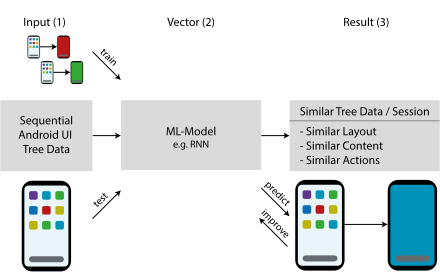
\includegraphics[width=\textwidth]{graphics/vectorization.svg}
  \caption{Possible procedure using a Machine-Learning algorithm to predict the next intent from a beginning user session: The input (1) can be a sequence of Android tree data. With help of a Machine-Learning-Model (2) (e.g. RNN) a vector representation can be trained and then predict the most probable action or screen (3) from a given starting sequence.}
  \label{fig:encode-decode}
\end{figure}

\begin{figure}
  \centering
  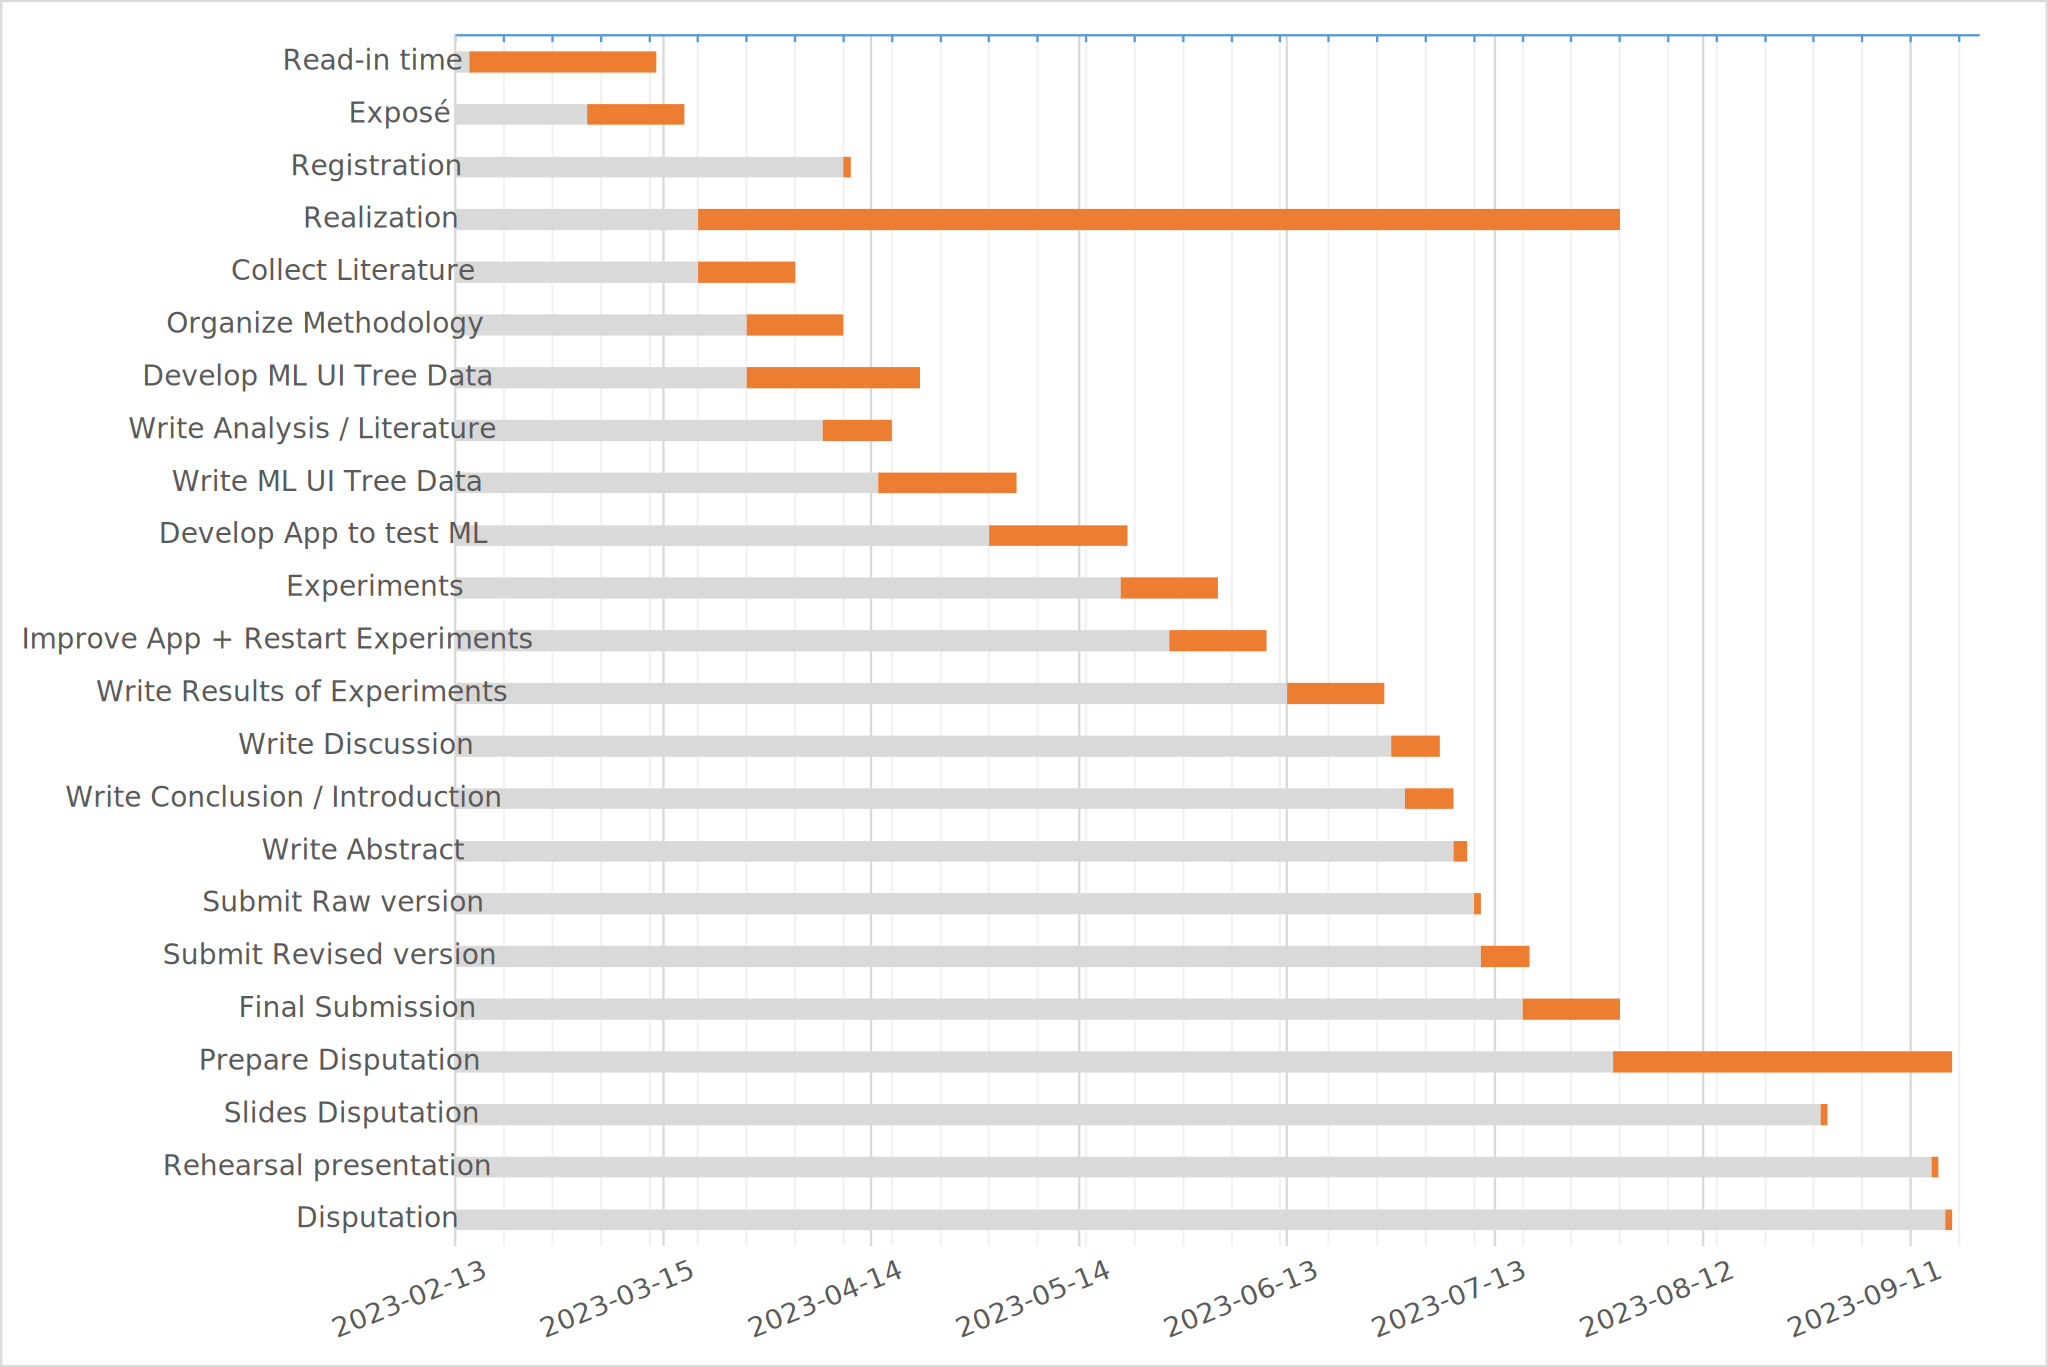
\includegraphics[width=\textwidth]{graphics/TimeTable-Gantt.svg}
  \caption{Schedule as a Gantt Chart}
  \label{fig:schedule}
\end{figure}


\cleardoublepage


% BEGIN: Verzeichnisse

\iftex4ht
\else
  \microtypesetup{protrusion=false}
\fi

%%%
% Literaturverzeichnis ins TOC mit aufnehmen, aber nur wenn nichts anderes mehr hilft!
% \addcontentsline{toc}{chapter}{Literaturverzeichnis}
%
% oder zB
%\addcontentsline{toc}{section}{Abkürzungsverzeichnis}
%
%%%

%Produce table of contents
%
%In case you have trouble with headings reaching into the page numbers, enable the following three lines.
%Hint by http://golatex.de/inhaltsverzeichnis-schreibt-ueber-rand-t3106.html
%
%\makeatletter
%\renewcommand{\@pnumwidth}{2em}
%\makeatother
%
\setcounter{secnumdepth}{4}
\setcounter{tocdepth}{4}
\tableofcontents

% Bei einem ungünstigen Seitenumbruch im Inhaltsverzeichnis, kann dieser mit
% \addtocontents{toc}{\protect\newpage}
% an der passenden Stelle im Fließtext erzwungen werden.

\listoffigures
\listoftables

% Control List of Listings
\let\iflistings\iffalse
%Wird nur bei Verwendung von der lstlisting-Umgebung mit dem "caption"-Parameter benoetigt
%\lstlistoflistings
%ansonsten:
\iflistings
  \ifdeutsch
    \listof{Listing}{Verzeichnis der Listings}
  \else
    \listof{Listing}{List of Listings}
  \fi
\fi

% Control List of Algorithms
\let\ifalgorithms\iffalse
\ifalgorithms
  %mittels \newfloat wurde die Algorithmus-Gleitumgebung definiert.
  %Mit folgendem Befehl werden alle floats dieses Typs ausgegeben
  \ifdeutsch
    \listof{Algorithmus}{Verzeichnis der Algorithmen}
  \else
    \listof{Algorithmus}{List of Algorithms}
  \fi
  %\listofalgorithms %Ist nur für Algorithmen, die mittels \begin{algorithm} umschlossen werden, nötig
\fi

% Control Glossary
\let\ifglossary\iftrue
\ifglossary
%  \setglossarysection{section} remove empty sites
%  \clearpage
  \printnoidxglossaries
%  \clearpage
\fi

\iftex4ht
\else
  %Optischen Randausgleich und Grauwertkorrektur wieder aktivieren
  \microtypesetup{protrusion=true}
\fi

% END: Verzeichnisse


% Headline and footline
\renewcommand*{\chapterpagestyle}{scrplain}
\pagestyle{scrheadings}
\pagestyle{scrheadings}
\ihead[]{}
\chead[]{}
\ohead[]{\headmark}
\cfoot[]{}
\ofoot[\usekomafont{pagenumber}\thepage]{\usekomafont{pagenumber}\thepage}
\ifoot[]{}


%% vv  scroll down for content  vv %%


%%%%%%%%%%%%%%%%%%%%%%%%%%%%%%%%%%%%%%%%%%%%%%%%%%%%%%%%%%%%%%%%%%%%%%%%%%%%%%
%
% Main content starts here
%
%%%%%%%%%%%%%%%%%%%%%%%%%%%%%%%%%%%%%%%%%%%%%%%%%%%%%%%%%%%%%%%%%%%%%%%%%%%%%%

\chapter{Introduction}
\label{sec:introduction}

This is a typical human-computer interaction thesis structure for an introduction which is structured in four paragraphs as follows:
% First Paragraph
% CORE MESSAGE OF THIS PARAGRAPH:

\section{The role of Intent Prediction}
\label{sec:role-intent-prediction}

The term \ti{intent} can have ambiguous meanings and can be used in different context.
In the dictionary it is described as the fact of intending something, so it is planned to do~\cite{dictionaryIntent}. % https://www.dictionary.com/browse/intent
Generally we can assume that intent is a stronger desire to accomplish ones intension.
Kofler and Hanjalic et al.~\cite{kofler2016user} also describe the intent as \quotes{immediate reason, purpose, or goal [\ldots] that motivates a user to} act.

The aim or purpose must be differentiated from the actual user input, also known as interaction.
So the intent can be seen as the preliminary stage of interaction.
Gestures and click sequences then are the concrete actions, and might fulfill a (small) part of the users intent.
Therefore, in this work it is not the goal to obtain the users full intent, but to work out factors, such as user inputs or gestures, which hint to the intent of the user.
Further, \ti{prediction} describes that the intent or factors of intent should be available (calculated) before they have actually happened or were measured.

\todo{Explain screen, view, flow, click}

But it can be easily replaced by more semantic data, which might even be easier to predict.
Descriptive User intent embedding as preliminary stage, which can be applied with Screen2Words\cite{screen2words} in a similar fashion.
difference intent / interaction / screen / flow / click


\section{Necessity of Vectors for Android UI}
\label{sec:necessity-of-vectors-for-android-ui}
\todo{Explain how many time a user spents on a mobile device, facilitate steps, make it more productive, qualitative user experience}


Motivation for transforming Android UI tree data to vectors

- open source code for predicting next user click / action
- evaluate and compare existing approaches
- provide tools to reduce screen sequences to vectors
- how to work with multidimensional (multi-modal) data in RNNs

- Low Button depth: number of clicks until one gets to the action \cite{lee2018click}

- Explain intent, and the other words in the title

Contributions: \cite{zhou2021large}
• An analysis of a large-scale dataset of mobile user click se-
quences that reveals rich factors and complexity in modeling
click behaviors, which contributes new knowledge to under-
stand mobile interaction behaviors.
• A Transformer-based deep model that predicts next element
to click based on the user click history and the current screen
and time. The model does not rely on a vocabulary of prede-
fined UI elements and provides a general solution for model-
ing arbitrary UI elements for click prediction.
• A thorough experiment that compares our deep model with
multiple alternative designs and baseline models, and an
analysis of model behaviors and benefits that the model can
bring to improve mobile interaction.

Contributions: \cite{li2021screen2vec}
Screen2Vec: a new self-supervised technique for generating
more comprehensive semantic embeddings of GUI screens
and components using their textual content, visual design
and layout patterns, and app meta-data.
(2) An open-sourced GUI embedding model trained using the
Screen2Vec technique on the Rico [9] dataset that can be
used off-the-shelf.
(3) Several sample downstream tasks that showcase the model’s
usefulness.

In computer science there often coexists multiple (correct) solutions to the same problem.
Many technologies have the capabilities of achieving a similar result, but are specialized in the one or the other way.
That led to the first question

\quotes{What is a suitable model for the prediction of user intent?}.

\quotes{At what level of detail the predictions can be made?}


\label{subsec:motivation}
\todo{P1.1. What is the large scope of the problem?}
\todo{P1.2. What is the specific problem?}

% Second Paragraph
% CORE MESSAGE OF THIS PARAGRAPH:
\todo{P2.1. The second paragraph should be about what have others been doing}
\todo{P2.2. Why is the problem important? Why was this work carried out?}

% Third Paragraph
% CORE MESSAGE OF THIS PARAGRAPH:
\todo{P3.1. What have you done?}
\todo{P3.2. What is new about your work?}

% Fourth paragraph
% CORE MESSAGE OF THIS PARAGRAPH:
\todo{P4.1. What did you find out? What are the concrete results?}
\todo{P4.2. What are the implications? What does this mean for the bigger picture?}

%LaTeX hints are provided in \autoref{chap:latexhints}.


\chapter{Theoretical Framework}
\label{ch:theoretical-framework}

Before starting with rehabilitate the main topic, some basic concepts, technical terms and underlying theory has to be explained.
This is important to faster read through the thesis without the need to interrupt the flow of thought.
In the following, a set of established theories and terms is explained which are not directly related to the thesis formulation, but essential to comprehend numerous contexts.

\section{Android UI}
\label{sec:android-ui}

To be able to use any of the things displayed on the mobile device, some concepts of \gls{ui} programming must be shown.
A \gls{ui} enables the user to view the applications data on the screen but also to interact with the device especially on mobile devices \cite{android_ui_layer}.

The main challenge is to bring the application data in the right format, so that the display can interpret the instructions to draw the elements.
Each mobile phone with the Android \gls{os} has a basic set of native functions through which the \gls{ui} can be drawn and updated, a so-called \gls{api}.
These functions can be very general to instruct drawing a whole component such as an alert box, or they can be very specific as drawing single rectangles in a canvas.

The rough transition from the application data (data layer) to the display data (ui layer) is depicted in figure \ref{fig:android_udf}.
The application data is transformed, concatenated or filtered to be saved in a view model, which represents the state for each view.
The view model is then layed out to multiple \gls{ui} elements.
E.g.\ they are loaded in the Android activity via view layouts~\cite{android_draw_views} or composed in a declarative approach~\cite{android_jetpack_compose}.
It is generally advised to use a \gls{udf}.
This ensures that the data is only changed in one place and doesn't get out of sync between \gls{ui} elements, the view model and the data layer.
The \gls{ui} can also register user inputs (like a button press) and report them back to the view model.
The view model then updates the application data, if needed, and then also reports the current \gls{ui} state back to the UI elements to be rerendered.

\begin{figure}[htbp!]
    \centering
    \begin{subfigure}[b]{0.5\textwidth}
        \centering
        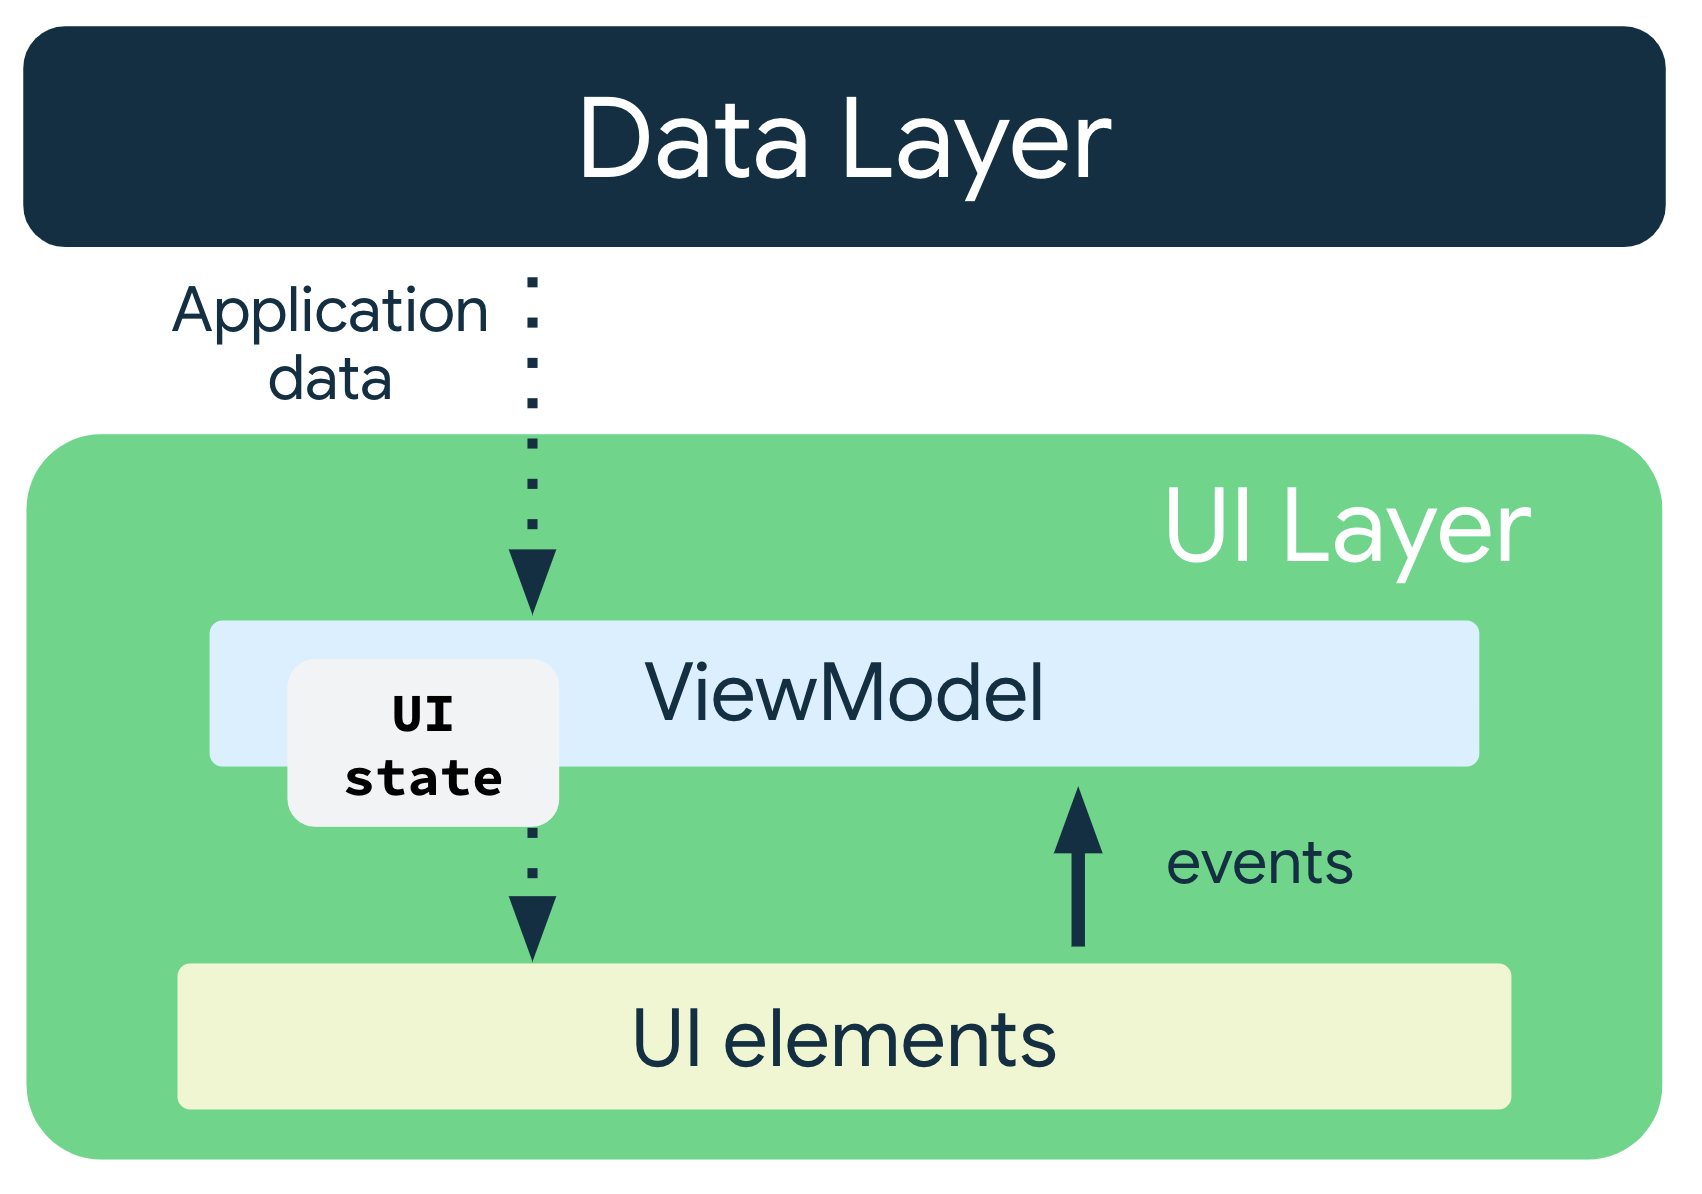
\includegraphics[width=\textwidth]{graphics/android_udf}
        \caption{Diagram of \gls{udf} in app architecture \cite{android_ui_layer}}
        \label{fig:android_udf}
    \end{subfigure}
    \hfill
    \begin{subfigure}[b]{0.4\textwidth}
        \centering
        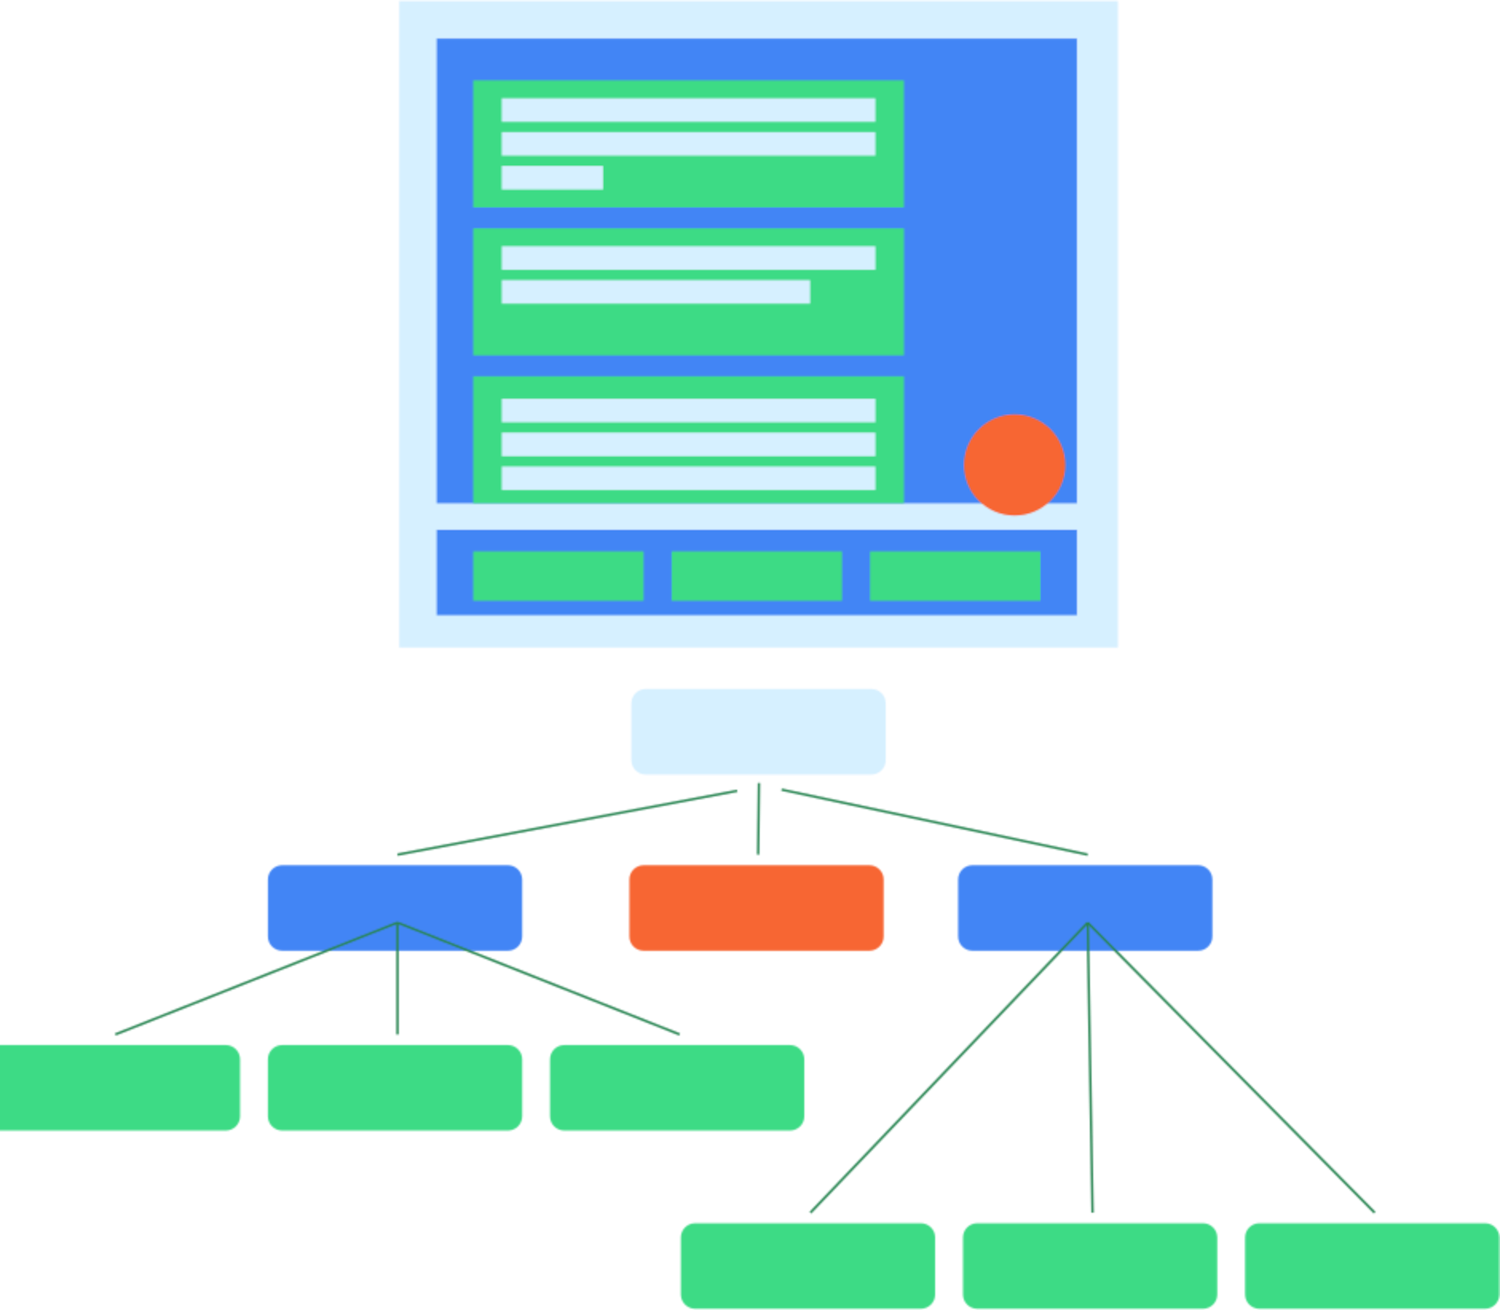
\includegraphics[width=\textwidth]{graphics/android_semantics-ui-tree}
        \caption{Schema of how the semantics tree is related to the \gls{ui} hierarchy \cite{android_semantics_compose}}
        \label{fig:android_semantics_ui_tree}
    \end{subfigure}
    \caption{Structure of the Android \gls{ui}}
    \label{fig:android_tree}
\end{figure}
%https://developer.android.com/guide/topics/ui/how-android-draws \cite{android_draw_views}
%https://developer.android.com/jetpack/compose/mental-model \cite{android_jetpack_compose}

\subsection{Data tree structure}
\label{subsec:data-tree-structure}

The \gls{ui} elements (i.e.\ the composition) themselves are hierarchically structured in a tree.
This allows the renderer to calculate relative distances, floatings and skip processing hidden or overlapped elements.

With the Android Layout Inspector (figure~\ref{fig:android_layout_inspector}) a view hierarchy tree can be visually inspected while displaying its position and layout on the Android screen.
Also, the layout attributes can be validated.
This tool allows to debug complex \gls{ui}s especially when using nested components and display them in a simplistic way.
Note that this tool is only available if one has access to the app's source code.

\begin{figure}[htbp!]
    \centering
    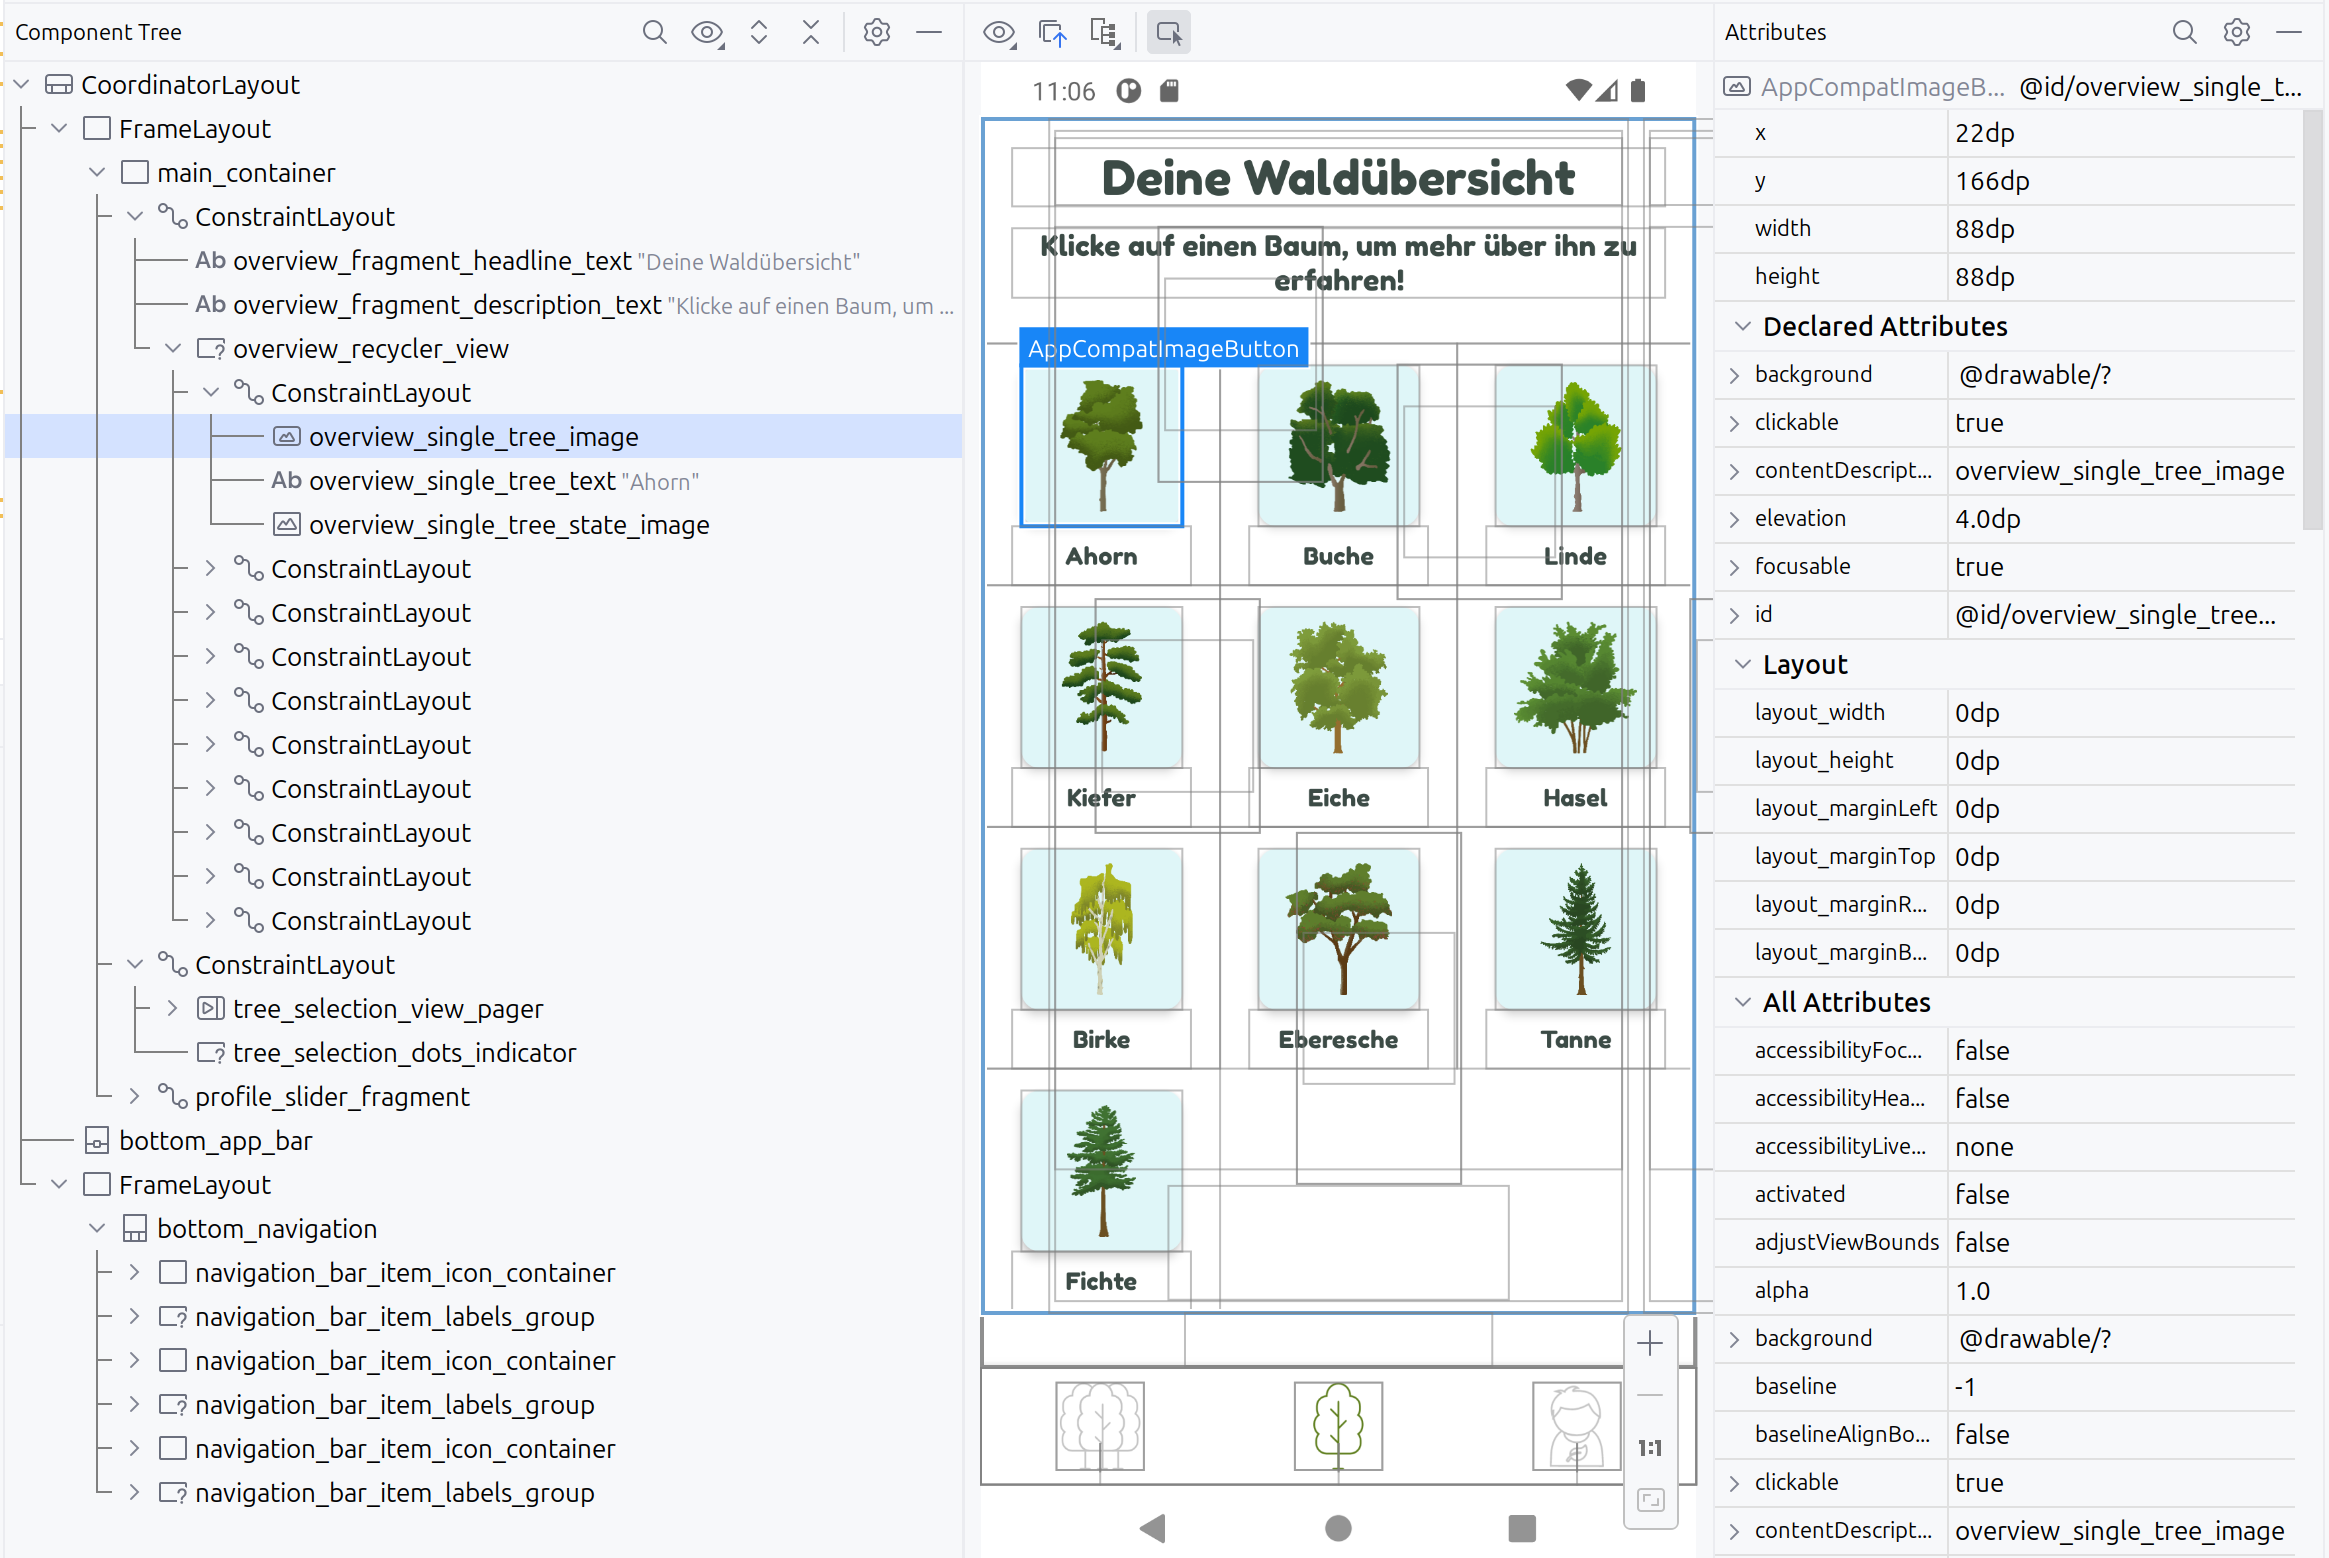
\includegraphics[width=\textwidth]{graphics/android_layout_inspector}
    \caption{The Android Layout Inspector tool using the example of \quotes{App ins Grüne}~\cite{mimuc_app_ins_gruene} by the Media Informatics Group of the LMU in Munich.}
    \label{fig:android_layout_inspector}
\end{figure}

\subsection{Android Accessibility Service}
\label{subsec:android-accessibility-service}

If an app is running in production on a users device, meaning that the app is compiled and publicly available, the ways of accessing the Android \gls{ui} tree are limited.
This behavior is of course wanted for safety and privacy reasons.
Nonetheless, if desired, a user can explicitly allow certain apps to gain access to the semantics tree of your Android \gls{os}.
This is especially useful for providing accessibility services for impaired users (like done with the TalkBack app).
Or -- as in our case -- the setting can be used to enable services which collect data for user studies or scientific experiments.

This semantics tree is deviated from the existing \gls{ui} tree.
It can be fed via special semantic properties while composing the \gls{ui}, e.g.\ by specifying the \code{contentDescription} property of an icon \cite{android_semantics_compose}.
Providing semantics is not limited to native platforms as shown by Flutter~\cite{flutter_semantics} and React Native~\cite{react_native_accessibility}.
In figure~\ref{fig:android_semantics_ui_tree} a schema is presented, which shows how the elements of the semantics tree are spanned compared to the components on the \gls{ui} layer.

%https://github.com/android/codelab-android-accessibility
To take advantage of the semantics tree, a custom accessibility service can be built, which can run in the background.
This service tracks all UI changes and has access to the current view hierarchy of the screen, which also inherits the semantic tree.
By altering the code of the \ti{AccessibilityNodeInfoDumper} one can extract the view hierarchy to a locale or remote database~\cite{android_accessibility_node_info_dumper}.
In the code section \ref{android_accessibility_node} a small fraction of a view hierarchy is shown.
It contains nested nodes with various attributes which represent the components of the combined \gls{ui} and semantics hierarchy.

%Semantics tree:
%https://api.flutter.dev/flutter/widgets/Semantics-class.html
%https://developer.android.com/jetpack/compose/semantics
%https://android.googlesource.com/platform/frameworks/testing/+/jb-dev/uiautomator/library/src/com/android/uiautomator/core/AccessibilityNodeInfoDumper.java \cite{android_accessibility_node_info_dumper}
%https://github.com/Gustl22/android-accessibility/blob/c158808533d6fc017455184a7317555d3e6946f6/GlobalActionBarService/app/src/main/java/com/example/android/globalactionbarservice/uiautomator/AccessibilityNodeInfoDumper.java

%Mean 18 actionable elements, with Std=12. \cite{zhou2021large}

\lstinputlisting[language=XML,label=android_accessibility_node,caption={Android Accessibility Node in XML.},float]{code/android_accessibility_node.xml}

\section{Machine Learning}
\label{sec:machine-learning}

\gls{ml}, a term spread by Arthur Lee Samuel, is a method of data analysis, more precisely a scientific approach to form statistical models without the need to explicitly program it~\cite{mahesh2020machine}.
It uses algorithms to iteratively learn how data is structured.
In contrast to statistical inference or manually crafted statistical models respectively, \gls{ml} can solve tasks by automation of model building.
Its advantages lie in finding hidden relations and patterns from the context, without having any or only a small pre knowledge of the data, thus it is a strong tool for generalization or abstraction of large datasets, also known as \gls{gl-bigdata}.
\gls{ml} can be applied to the following fields among others: email and spam filtering, fraud detection, cybersecurity, web search engines, recommender systems (like known from Netflix or Amazon), advertising, translators and text generation, pattern and image recognition.
The data driven approach also comes with some drawbacks: the outcome heavily depends on the provided data.
It can include biases and therefore may acquire forms of discrimination or unfair treatment.
Nonetheless \gls{ml} has a lot of potential to uncover hidden connections in large datasets.


\todo{explain Tensors, Datasets}
%https://stackoverflow.com/a/48599383/5164462

\subsection{Preprocessing}

Preprocessing describes the step after one acquired their data, but before training the \gls{ml} model.
This step is not to be underestimated.
A \gls{ml} model can perform significantly better when certain preprocessing steps are applied \cite{alam2019impact}.

To be able to preprocess, we have to know with what kind of data we handle with.
Data entries can occur in different forms, but we can break them down in three main types:
\begin{itemize}
    \item \tb{Categorical values}: a value is always assigned to a class with a fixed pool of predetermined classes.
          E.g.\ letters, words, brands, animals, chemical elements
    \item \tb{Continuous values}: the value can be fractional and may lies in between a lower and an upper bound.
          E.g.\ temperature, velocity, geographic position
    \item \tb{Integer values}: the value is a whole number and may also lie in between a lower and an upper bound.
          E.g.\ revolutions per minute, product number, annual sales
\end{itemize}

For discrete and continuous values, we have a wide variety of options for preparing them in order to be subsequently processed by a \gls{ml} model \cite{duong2021}.


\subsubsection{Feature selection}

Feature selection is a crucial step to successfully develop a model with the desired results.
It can improve learning performance, thus reduces time, increases computational efficiency, decreases memory storage, and helps build better generalization models \cite{li2017feature}.
Also, it may be a valid approach to get around missing data and can help structure the data by removing unnecessary clutter.

%https://dl-acm-org.emedien.ub.uni-muenchen.de/doi/pdf/10.1145/3136625
On the technical sight, feature selection can be differentiated for two goals: supervised and unsupervised learning~\cite{li2017feature}.
However, principles from the supervised feature selection can be applied in the unsupervised domain, resulting in a semi-supervised filter selection.
For classifiers and regression problems (unsupervised) following methods can be applied.
Multiple features can be compared by calculating their correlation.
If one feature is uncorrelated to all other features, this may be an indicator that this feature can be dropped, as it may doesn't contribute to the resulting model (\ti{filter method}).
However, this can only be stated for linear correlations, thus it may contribute to the result in an unpredicted way.
Also, if two features correlate too much to each other, one feature may is redundant and can be dropped.
A good approach is also to reduce the dimensionality of the input data, e.g.\ by replacing \ref{one-hot} encoded features of the same domain with embeddings (\ti{embedded method}).
This is also called \ti{feature extraction}.
Feature extraction can also be used in unsupervised feature selection.
Clustering is a common approach to reduce the number of input dimensions by gaining insights of which classes can be merged and which need to stay.
A more computational but promising solution is to filter the features by optimizing the model result, also called a \ti{wrapper method}.
By gradually removing and adding features and calculating the models performance, one can determine which inputs are important and which may only steal computing time.

semantic or legal feature selection
Such as Filtering privacy invasive details
Remove sensitive data
%https://news.mit.edu/2023/new-way-look-data-privacy-0714

Parameterizing the vectorization process
a) Vector length
b) Weighting of features
c) Manipulating individual parameters of model

\subsubsection{Missing data}
Some data entries may are missing.
Therefore, you have two approaches to get around these missing values.
One can drop these values by removing the column or row.
This is only recommended if you are not relying on this data entry, or this the whole feature is not expected to be important enough to bring any value to the model's performance.
Further you can fill the data with a default value like zero or calculate a reasonable value from the surrounding data entries by taking their \quotes{mean, median, or interpolation}~\cite{duong2021}.
The second approach can only be applied to numerical data.

\subsubsection{Normalization and Standardization}

This is only applicable for numerical data.
Many \gls{ml} models work better or exclusively with normalized data.
This means that the values have to be in a certain range, most commonly are from \tb{0} to \tb{1} or from \tb{-1} to \tb{1}.
This can be achieved by dividing all values with the difference of the minimum and maximum value and shift the output accordingly \cite{duong2021}.

% X new = (X — X min)/ (X max — X min)

Sometimes this is not enough, e.g.\ if having a few extreme values, and an approach is desired which better reflects the average data.
Here the standardization, also called z-score normalization, comes into play.
This method scales the values so that the mean value is placed at \tb{0} and the standard deviation is placed at \tb{1}.
%https://medium.com/analytics-vidhya/what-are-data-standardization-and-data-normalization-f880dd9e79b6
\subsubsection{Padding}


\subsubsection{Categorical Variables}

\todo{categorical}
According to \cite{alam2019impact} these steps can be removal of emoticons, elimination of stopwords and stemming for text based models.

ordinal categories belong to the \tb{Integer values} as they

Category Embedding before LSTM
% https://stackoverflow.com/questions/47217151/keras-lstm-with-embedding-layer-before-lstm-layer
% https://stackoverflow.com/questions/52627739/how-to-merge-numerical-and-embedding-sequential-models-to-treat-categories-in-rn/52629902#comment136040845_52629902


- Embedding layer
Embedding dimension is about the actual voc\_size, but not too large.
Dimension near the actual average length of features (?)

\subsection{Supervised vs Unsupervised vs Semisupervised}

\subsubsection{Supervised Learning}
Supervised: Classification and regression
Uses \tb{labeled} examples: Input and output is known

Learns by comparison of the output it is provided with the output the model \ti{predicts}.

Steps:
- Data acquisition
- Data cleaning / Preprocessing (Panadas)
- Split into Training Data, Validation data, and Test data (cannot adapt the model after using the test data)
- Train the model with the train data
- Evaluate the model with the test data, then can adapt the model by the developer
- Last deploy the model to production

\subsubsection{Unsupervised Learning}
Clustering
Reinforcement learning

self-supervised

\subsection{Under and Overfitting}
\label{subsec:under-and-overfitting}


\section{Artificial Neural Nets}
\label{sec:artificial-neural-nets}

- Uses biological neuron systems as paradigm to generate mathematical models
- can solve tasks by abstraction or generalization of data relations


Activation Functions
Cost function
Gradient
- Regression: Continous Values
- Classification: Multiple class
- One Class

\subsection{Classes of Neural Nets}
\label{subsec:classes-of-neural-nets}

\subsubsection{Deep Neural Nets}

Neural Net with more than one layer
- Dense Layer

\subsubsection{Convolutional Neural Nets}
\subsubsection{Recurrent Neural Networks and LSTMs / GRU}
LSTM 4 dimensional
% https://stackoverflow.com/questions/54743549/is-it-possible-to-making-lstm-model-with-4-dimension-shape-of-data

Limitations to only 3 dimensions, needs flattening

Sample dimension (X -> y)
Time (Step) Dimension
Feature Dimension
Data, Quantity dimension, such as Image dimensions, or multiple nodes

TimeDistributedLayer
% https://stackoverflow.com/a/61588937/5164462
% https://stackoverflow.com/questions/53107126/what-are-the-uses-of-timedistributed-wrapper-for-lstm-or-any-other-layers

\subsubsection{Autoencoders}
\label{subsubsec:autoencoder}

Encoder, Decoder

\subsection{Tensorflow and Keras}
Layers
FlattenLayer

Positive Integer to Dense Vectors of fixed size

\section{Evaluation and Metrics}
\subsection{Mean Squared Error}
\subsection{F1 Score}


\chapter{Related Work}
\label{ch:related-work}

\todo{introduce in related work, differentiate the importance of datasets}
Describe relevant scientific literature related to your work.

%%%%%%%%%%%%%%%%%%%%%%%%%%%%%%%%%%%%%%%%%%%%%%%%%%%%%%%%%%%%%%%%%%%%%%%%%%%%%%%%

\section{Datasets of UI Trees}
\label{sec:datasets-of-ui-trees}

Requirements on a good data set
- Google and Samsung
- need to have correct data
- needs enough data to train a NN
- need enough features to be able to recognize patterns
- up to date
- Publicly available
- Variable length of app sessions, define one session of activating the screen until it is turned off.

Missing
- System to feed in in real time
- Dataset which is across multiple apps, also tracks the system
-

\subsection{ERICA}
\label{subsec:erica}

ERICA is a design and interaction mining application, which allows gathering \ti{interaction traces} by capturing the users activity on Android apps~\cite{deka2016erica}.
This is accomplished through a web-based interaction layer in contrast to the other common approach of using \ti{accessibility services} directly.
They justify that approach by the lack of need to install additional applications, as only a browser is required.
A further reason is the response latency of the commonly used \ti{UiAutomator}, which cannot collect the data in time.
Also they argue that capturing and simultaneously interacting with the apps may overload the user device and challenges the user experience.
Therefore the much more powerful servers take the task of capturing the UI trees.
The apps are hosted on multiple physical devices with a modified Android OS directly connected with the server.
ERICA captures UI screens and user flows by tracking UI changes.
They then used this data to form k-mean clusters from the UI elements (visual and textual features) and the interactive elements (icons and buttons).
Based on the clusters they then build classifiers and trained an AutoEncoder (\ref{subsubsec:autoencoder}) to determine the flows from the test dataset.
The authors worked out 23 common user flows (from over a thousand popular Android apps) which aim to provide complementary, promising or new design patterns and trends.

%- data-driven app design application
%- gathers user interaction trace > 1000 popular apps
%- 3000 flow examples

%\todo{descibe how they worked out the 23 user flows, which Autoencoder they used etc.}

\subsection{Rico / RicoSCA}
\label{subsec:rico}

Rico \cite{deka2017rico} (spanish for \quotes{rich}) is the successor of ERICA.
It aims to help perform better at designing and support the creation of adaptive UIs.
As far as known to date this is the largest collection of mobile app designs and traces with covering 72k UI screens in 9.7k Android apps.
Like its predecessor Rico uses a web-based approach to collect user traces.
It enables the applications like searching for designs, generation of UI layouts and code, modeling of user interactions, and prediction of user perception.
It exposes visual, textual, structural, and interactive design properties of more than 72k unique UI screens.
Unfortunately the dataset doesn't include interaction traces for app to app transitions or interactions with the Android OS itself.
In table~\ref{tab:rico_view_hierarchy_attributes} a collection of all view hierarchy attributes is shown with their meaning.
These were extracted by iterating over all view hierarchy files contained in the traces of the dataset.
This gives insights in what attributes were recorded in the Rico dataset and what relevance they may have during training the model.
The authors of Rico used their dataset to train a 64-dimensional UI layout vector~\ref{subsubsec:embedding} with an AutoEncoder \ref{subsubsec:autoencoder}.
For their input they converted the UI layout hierarchy to an image with colored bounding boxes differentiating images and text.
This has the advantage to be able to deal with the high dimensions inside the UI tree.
But the conversion also most likely discards lots of meaningful information hidden in the UI tree semantics.

\begin{table}[htbp!]
  \small
  \centering
  \begin{tabular}{|l|c|c|>{\RaggedRight}p{0.5\linewidth}|}
    \hline
    \tb{Key} & \textbf{Type} & \textbf{Shape} & \textbf{Description} \\
    \hline
    \multicolumn{4}{c}{Per View} \\
    \hline
% Annotated by word2vec
%    \_is\_leaf\_node & bool & (1) & \\
%    \_caption\_preorder\_id & bool & (1) & \\
%    \_caption\_depth & bool & (1) & \\
%    \_caption\_node\_id & bool & (1) & \\
%    \_caption\_postorder\_id & bool & (1) & \\
    activity\_name & string & (1) & Name of the activity: e.g. \quotes{com.my\_app.AppName.MainActivity} \\
%    added\_fragments & [] & (None) & \\
%    active\_fragments & [] & (None) & \\
    is\_keyboard\_deployed & bool & (1) & Indicates if the keyboard is shown \\
    request\_id & int & (1) & Id used by the crawler to request the view \\
    \hline
    \multicolumn{4}{c}{Per Node} \\
    \hline
    abs-pos & bool & (1) & Indicates if position in \ti{bounds} is relative or absolute; if \ti{true}, \ti{rel-bounds} is set \\
    adapter-view & bool & (1) & Indicates that children are loaded via an adapter, see~\cite{android_adapterview} \\
    ancestors & [string] & (None) & Ancestors of current node, e.g. \quotes{android.view.View} \\
    bounds & [integer] & (4) & Absolute or relative boundaries, dependent on \ti{abs-pos} \\
    children & [node] & (None) & Child nodes \\
    class & string & (1) & \quotes{com.my\_app.lib.ui.views.DropDownSpinner} \\
    clickable & bool & (1) & User can interact by press / click \\
    content-desc & string & (1) & (Accessibility) description of the node \quotes{Interstitial close button} \\
    draw & bool & (1) & Indicates if this node is drawn on the canvas \\
    enabled & bool & (1) & Indicates if this node is in the enabled state \\
    focusable & bool & (1) & Indicates if this node can be focused \\
    focused & bool & (1) & Indicates if this node can is currently in focus \\
    font-family & string & (1) & States the font family, e.g. \quotes{sans-serif} \\
    long-clickable & bool & (1) & Indicates if this node has a long press action \\
    package & string & (1) & States which packages the node belongs to \quotes{com.my\_app.mypackage} \\
%    pointer & string & (1) & \todo{Presumably the saving address in the memory, e.g. \quotes{92690f4}} \\
    pressed & bool & (1) & Indicates if this node can is currently pressed \\
    rel-bounds & [integer] & (4) & Relative boundaries, if \ti{abs-pos} is set to \ti{true} \\
    resource-id & string & (1) & The unique resource identifier for this view \quotes{android:id/navigationBarBackground} \\
    scrollable-horizontal & bool & (1) & Indicates if this node can be scrolled horizontally \\
    scrollable-vertical & bool & (1) & Indicates if this node can be scrolled vertically \\
    selected & bool & (1) & Indicates if this node can is currently selected \\
    text & string & (1) & Text value if this node is a textual element \\
    text-hint & bool & (1) & Explanation text for text boxes or icons \\
    visibility & string & (1) & Indicates if this node is hidden, e.g. \quotes{visible}, \quotes{gone}\\
    visible-to-user & bool & (1) & Indicates if this node can be seen in the viewport by the user \\
    \hline
  \end{tabular}
  \caption[Attributes of a view hierarchy record]{Collection of attributes of a \ti{view hierarchy} record, extracted from all interaction traces of the Rico \cite{deka2017rico} dataset.}
  \label{tab:rico_view_hierarchy_attributes}
\end{table}

The RicoSCA dataset has been formed out of the research topic of mapping language instructions to mobile UI action sequences~\cite{li2020mapping}.
They removed screens whose bounding boxes in the view hierarchies are inconsistent with the screenshots with the help of annotators.
The process of filtering reduced the Rico dataset to 25k more concise and meaningful screens.

\subsection{Mobile UI CLAY Dataset}

The Google researchers Gang Li et al. \cite{clay} present a a so-called \ti{CLAY} pipeline which is able to denoise mobile UI layouts from incorrect nodes or adding further semantics to it.
As basis they used the Rico \ref{rico} dataset for a subject of improvement.
They state that recording results are dynamic and can get out of sync with the actual screen of the user.
That leads to 37.4\% of screens which contain invalid objects.
This induces invisible or misaligned objects, or objects which are not clickable (greyed out).
The researchers filtered invalid objects by training a \gls{resnet} model with the screenshots to classify nodes as as invalid if their bounding boxes don't match.
Also they introduced two models: a \gls{gnn} and a Transformer model to each determine the view type (also related to the view class).
For that they considered the view hierarchy attributes as well as the screenshots via a \gls{cnn}.
They claim they outperform heuristic approaches for detecting layout objects without a visual valid counterpart and also can recognize their types in more than 85\%.
This pipeline could help to improve intent prediction algorithms as less inconsistent data is applied to the model.

%%%%%%%%%%%%%%%%%%%%%%%%%%%%%%%%%%%%%%%%%%%%%%%%%%%%%%%%%%%%%%%%%%%%%%%%%%%%%%%%

\section{Vector models}

- Compress a huge data set to a concise model
- Vector Representation enables

Advantages:
- \quotes{small} or smaller than the data set itself
- No need to have pre knowledge about the topic, just need input an output (labels) for unsupervised NN
-

\subsection{Doc2Vec and Word2Vec}
%http://proceedings.mlr.press/v32/le14.pdf
%6_Quoc-Le_Doc2Vec
\cite{le2014distributed}

\subsection{Screen2Vec}
\label{subsec:screen2vec}

Toby Jia-Jun Li, Lindsay Popowski et al. \cite{li2021screen2vec} wrote a \gls{nn} called Screen2Vec which embeds the UI components while preserving the semantics.
%i.e., the type of machine learning approach that trains a model without human-labeled data by withholding some part of the data, and tasking the network with predicting it
It is claimed that they are among the first to develop a \gls{nn} for mobile screens which takes textual, visual design, and layout patterns and app context meta-data into account.
As inspiration they used the Word2Vec~\ref{word2vec} to predict result by considering the context and map them to a \gls{cbow}.
The self-supervised~\ref{self-supervised} model consists of two pipeline levels.
The outer level (\gls{gui} screen level) combines embeddings of \gls{gui} components, layout hierarchy and app descriptions.
The inner level is only present for the \gls{gui} components as they contain nested embeddings for the screen text and the class type.
The screen text (in the inner level) as well as the app description (in the outer level) is processed using a pretrained Sentence-BERT model.
The layout hierarchy is converted to a colored image encoding the text and image boundaries with colors (like in~\ref{subsec:rico}).
With such model, a vector can be calculated for each screen which then can be compared to each other, e.g.\ by the euclidean distance between the pixel representations, or comparing the distance in the view hierarchy representation.
When taking all features into account, both, the euclidean and the hierarchical approach, get an \gls{gl-accuracy} of around 0.85 that the correct screen is among the first 1\% of the models predictions.
In around half of the cases the predicted screen (\quotes{Top-1 Accuracy}) is the correct one.

Such an approach of representing an Android layout and context in a vector can be used as pretrained embedding for feeding a \gls{rnn} predicting upcoming screens.

\subsection{Screen2Words}
\label{subsec:screen2words}

Similar to \cite{li2021screen2vec} Screen2words considers the screen context from the view hierarchy to create a screen embedding.
The goal is to provide a summarization for an unseen screen by usage of it's app and \gls{ui} context.
They describe such a technique as multi-modal, as it \quotes{leverages input from multiple data sources}, like screenshot images, textual labels and UI tree structures.
As basis for their training data the Rico-SCA \ref{subsec:rico} dataset is used, to remove inaccurate view hierarchies.
Although the public code did not provide a direct way to parse the \gls{gl-protobuf} of Rico-SCA.
In addition they hired 85 labelers to manually annotate each of the 22k existing screens with multiple summarizations, resulting in more than 100k phrases.

As input for their summarizing \gls{nn} they used a flattened view hierarchy which contained padded embeddings for categorical values, like the view class.
Also the textual components of the screen were extracted and encoded with a pre-trained GloVE Word embedding.
The GloVE encoding was also applied to the app description.
The description was combined with the textual components and the other screen attributes to serve as input of a Transformer Encoder \ref{subsubsec:transformer}.
Simultaneously each screenshot was embedded though a \gls{cnn}, which was then concatenated with the Transformer Encoder to form the overall encoder of the Screen2words model.
The screen summaries were used as labels for the model and were also embedded with the GloVE encoding.

%\todo{experiment results} how to compare BLEU CIDEr ROUGE-L etc. distances
%- screen summarization
As human validation they made a study consisting of more than a thousand participants.
These had to give a star rating from one to five to assess the quality of the screen summarization.
They also trained different graduations of their model by removing some of their modalities.
That showed that using all modalities brought the best results (3.4 stars mean) in their rating.
Using only the screenshots (pixel) modality the ratings were lower by almost one star indicating that adding more modalities contribute to improve the screen to word vectorization.

\todo{why this paper is important for this work}
- can give insights in evalutation methods
- uses good embedding for various input modalities
- has a solution to embed words

\subsection{Intention2Text}
\cite{yu2020understanding}

\subsection{Html2Vec}
\cite{wu2022distributed}

\subsection{Tree2Vec}

\subsection{Activity2Vec}

%%%%%%%%%%%%%%%%%%%%%%%%%%%%%%%%%%%%%%%%%%%%%%%%%%%%%%%%%%%%%%%%%%%%%%%%%%%%%%%%

\section{Time Series / Sequence models}

- one more dimension
- allows predicting unseen states
- back propagation -> see technical part
-

RNNs: 9\_Personalizing session based recommendations with RNNs \cite{quadrana2017personalizing}
10\_Bansal\_Hybrid RNN Recommender system \cite{bansal2022remembering}
\cite{pietro2022recommendationSystems}

\subsection{Seq2Seq Model}
\cite{chollet2017seq2seq}

\subsection{Click Sequence Prediction / PathFinder}

Seokjun Lee et al. \cite{lee2018click} propose a technique called \ti{PathFinder} which aims to predict the sequence of user clicks in Android mobile apps.
The user input and the contextual data is collected via the Android Accessibility Services \ref{accessibility_services}, so the users \gls{os} does not need to be modified or \glslink{gl-rooting}{rooted}.
They collected the data from 55 students of their university with a sequence tracing tool and collected near 2 million button clicks from over a thousand apps.
They follow a collaborative and content-based approach which takes both all the users data as well as the individual preferences into account.
The \ti{button depth} describes the number of clicks or taps until the user gets to their target screen.
In average nearly the user has 16 buttons as candidates to press as the next action.
With a personalized UI a the \ti{button depth} should decrease significantly.
The next user click is dependent on very recent but also on previous clicks happened a longer time ago, e.g.~taking a picture relates to uploading it later to their \gls{sns}.
The authors train a \gls{lstm} model to predict the next button, which will be clicked on.
PathFinder predicts the most probable three buttons with a 0.76 F-measure.

In contrast to this work, \ti{PathFinder} does not take into account the complete view hierarchy or other spatiotemporal information.
Just the previous and the current app and the click history with their button properties are considered.
Also as far as known the dataset and code is not publicly accessible.

% "Very challenging to make accurate predictions of the click sequence."

\subsection{Large-Scale Modeling of Mobile User Click Behaviors Using Deep Learning}
\label{subsec:user-click-behaviors-deep-learning}

Xin Zhou and Yang Li \cite{zhou2021large} extend the work of \cite{lee2018click}.
They expect to optimize the UI experience by recommending the users next click interaction based on their findings.
They gathered a dataset of 20 million clicks from 4k mobile users.
The goal was to overcome the challenge of accurate but also scalable click sequence modeling.
That means that apps are not limited in their composition and the screens get increasingly diverse and there's no predefined set of UI elements.
Also the users click behavior is very individual and heavily dependents on situational factors.

Based on the Transformer architecture in \ref{subsubsec:transformer} they created a deep learning model which has 48\% \gls{gl-accuracy} for predicting the next user click and 71\% \gls{gl-accuracy} for the three most probable \ti{actionable} objects.
The researchers differentiated three main inputs for embedding their elements visible on the screen: the text content, the type of view and the bounding box.
All the elements are then passed to a Transformer Encoder representing a single screen.
Together with the click event as well as the time encoding the screen embedding serves as one concatenated input step.
The encoded time can be very different as it doesn't follow a regular sample interval, but is recorded as soon as the screen is changing \ref{fig:zhou_event_time_intervals}.
Multiple input steps then form a sequence fed in a second Transformer Encoder which contains all past screens and clicks.
The current screen embedding and time are then passed to a pointer (M-layer perceptron) which calculates the most probable \ti{actionable} elements to be clicked on.
They consider a UI element as \ti{actionable}, if it is currently \code{clickable}, \code{visible} and \code{enable}d (cf.\ table~\ref{tab:rico_view_hierarchy_attributes}).
More complex screens can have much more actionable elements, which makes the prediction much more difficult~\ref{fig:zhou_actionable_elements}.
% They introduced another metric to measure such predictions, which are relative to the number of objects.

This paper solves a lot of problems previous attempts had.
The dataset includes cross-app transitions which make 26\% of all clicks, which are also considered in their model.
The current context was taken into account such as the time of the day and day in the week~\ref{fig:zhou_event_time_distribution} which adds a lot of semantics.
Further they used a transformer model with self-attention, which reduces the training times significantly compared to \gls{lstm}.
Compared to the approach tested in this paper, they also predict the concrete element that will be clicked on instead of the absolute screen coordinates.

Unfortunately as far as the investigation permits, neither the dataset nor the code were publicly provided.

\begin{figure}[htbp!]
  \centering
  \begin{subfigure}[b]{0.3\textwidth}
    \centering
    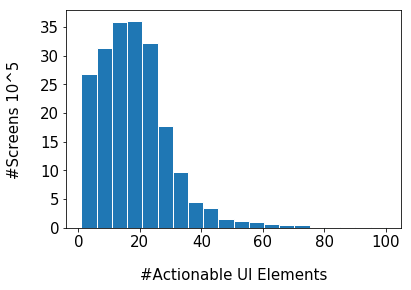
\includegraphics[width=\textwidth]{graphics/zhou_actionable_elements}
    \caption{Number of actionable elements per screen}
    \label{fig:zhou_actionable_elements}
  \end{subfigure}
  \hfill
  \begin{subfigure}[b]{0.3\textwidth}
    \centering
    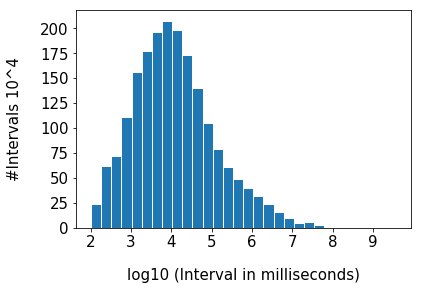
\includegraphics[width=\textwidth]{graphics/zhou_event_time_intervals}
    \caption{The distribution of time intervals between click events}
    \label{fig:zhou_event_time_intervals}
  \end{subfigure}
  \hfill
  \begin{subfigure}[b]{0.3\textwidth}
    \centering
    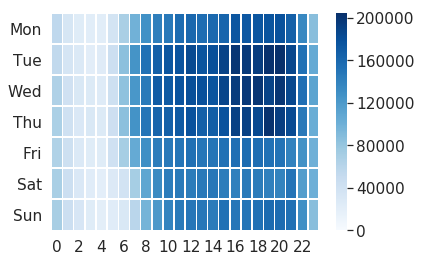
\includegraphics[width=\textwidth]{graphics/zhou_event_time_distribution}
    \caption{The distribution of time intervals between click events}
    \label{fig:zhou_event_time_distribution}
  \end{subfigure}
  \caption{View element insights \cite{zhou2021large}}
  \label{fig:zhou_graphs}
\end{figure}


\chapter{Methodology}

Start with your overall approach to the research. What research problem or question did you investigate? What type of data did you need to answer it? Quantitative, qualitative, or mixed? Primary or secondary? Experimental or descriptive?
Describe the specific methods you used for data collection and analysis. How did you collect and analyze your data? What tools or materials did you use? How did you ensure the quality and accuracy of your data?
Explain why you chose these methods over others. How do they relate to your research question and literature review? How do they address the limitations or gaps in existing research? How do they suit your research design and objectives?
Evaluate and justify your methodological choices. How did they affect the outcome of your research? What challenges or difficulties did you encounter and how did you overcome them? How can you ensure the credibility and generalizability of your findings?

How this thesis is working?
Apparatus, Procedure, Utilities


\section{Android UI Data}
\subsection{Data tree structure}

\begin{figure}
    \centering
    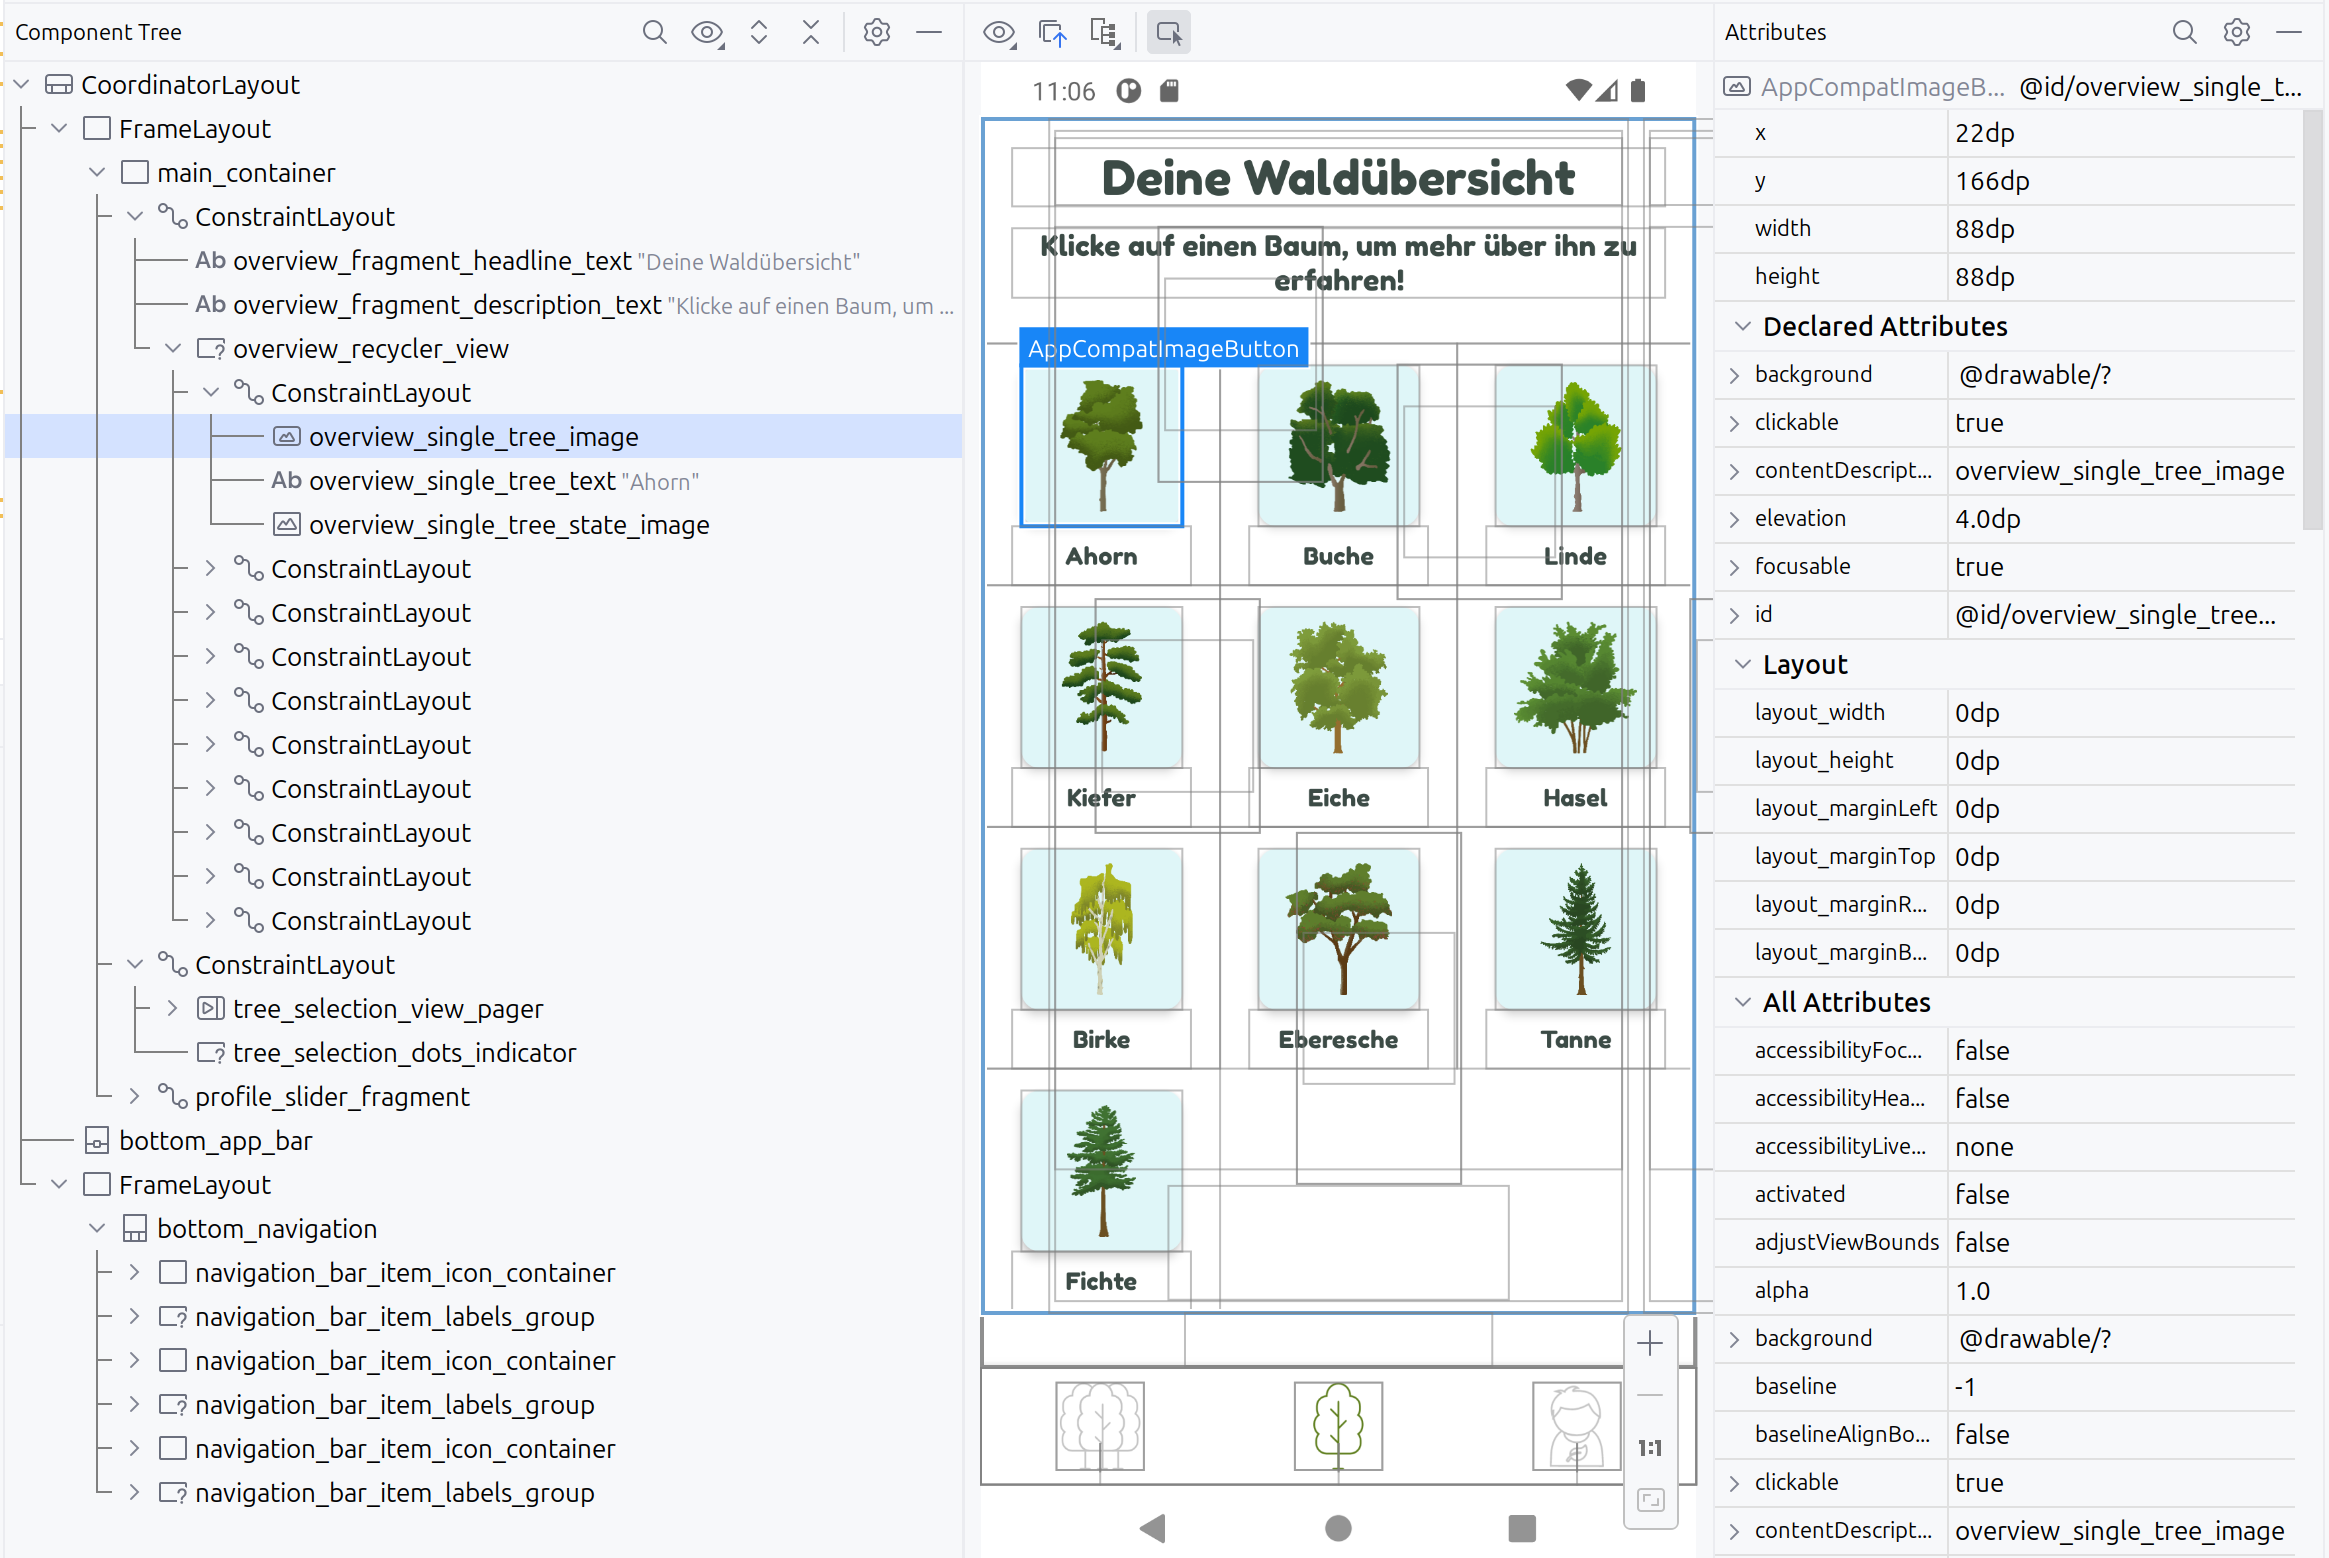
\includegraphics[width=\textwidth]{graphics/android_layout_inspector}
    \caption{https://developer.android.com/studio/debug/layout-inspector, https://github.com/mimuc/app-ins-gruene}
    \label{fig:android_layout_inspector}
\end{figure}

\subsection{Retrieval of UI data via Android Accessibility Service}

Semantics tree:
https://developer.android.com/jetpack/compose/semantics
https://android.googlesource.com/platform/frameworks/testing/+/jb-dev/uiautomator/library/src/com/android/uiautomator/core/AccessibilityNodeInfoDumper.java
https://github.com/Gustl22/android-accessibility/blob/c158808533d6fc017455184a7317555d3e6946f6/GlobalActionBarService/app/src/main/java/com/example/android/globalactionbarservice/uiautomator/AccessibilityNodeInfoDumper.java

\lstinputlisting[language=XML,label=android_accessibility_node,caption={Android Accessibility Node in XML.},float]{code/android_accessibility_node.xml}

\section{Machine Learning}
\subsection{Preprocessing}

Tensors, Datasets
%https://stackoverflow.com/a/48599383/5164462

\subsubsection{Feature selection}
Such as Filtering privacy invasive details

Parameterizing the vectorization process
a) Vector length
b) Weighting of features
c) Manipulating individual parameters of model

\subsubsection{Normalization}



\subsubsection{Padding}

\subsubsection{Embedding}

Category Embedding before LSTM
% https://stackoverflow.com/questions/47217151/keras-lstm-with-embedding-layer-before-lstm-layer
% https://stackoverflow.com/questions/52627739/how-to-merge-numerical-and-embedding-sequential-models-to-treat-categories-in-rn/52629902#comment136040845_52629902


- Embedding layer
Dimension near the actual average length of features (?)

\subsection{Supervised vs Unsupervised vs Semisupervised}
Reinforcement learning
\subsection{Under and Overfitting}
\subsection{Evaluation Metrics}
\section{Artificial Neural Nets}
Activation Functions
Cost function
Gradient
- Regression: Continous Values
- Classification: Multiple class
- One Class

\subsection{Classes of Neural Nets}

\subsubsection{Deep Neural Nets}
- Dense Layer

\subsubsection{Convolutional Neural Nets}
\subsubsection{Recurrent Neural Networks and LSTMs / GRU}
LSTM 4 dimensional
% https://stackoverflow.com/questions/54743549/is-it-possible-to-making-lstm-model-with-4-dimension-shape-of-data

Limitations to only 3 dimensions, needs flattening

Sample dimension (X -> y)
Time (Step) Dimension
Feature Dimension
Data, Quantity dimension, such as Image dimensions, or multiple nodes

TimeDistributedLayer
% https://stackoverflow.com/a/61588937/5164462
% https://stackoverflow.com/questions/53107126/what-are-the-uses-of-timedistributed-wrapper-for-lstm-or-any-other-layers

\subsubsection{Autoencoders}

Encoder, Decoder

\subsection{Tensorflow and Keras}
Layers
FlattenLayer

Positive Integer to Dense Vectors of fixed size

\section{Evaluation and Metrics}
\subsection{Mean Squared Error}
\subsection{F1 Score}


\chapter{Results}
\label{ch:results}

%A concept will be developed on how a model for predicting user intent could be built and how it could be applied to the user session.
%To this end, possibilities for collecting and vectorizing sequential UI trees will be discussed
%which are designed to predict the user intent. Here, privacy and feature pre-filteringin UI data plays an important role
%
%After that, personalized as well as collaborative data can be used in a hybrid approach.
%This modelshould then be made available to the user in an Android app service and, depending on the level ofdetail, suggest upcoming apps or actions to the user at a suitable time

This chapter will explain how a prediction model for user intent can be designed and what factors of influence have to be considered.
The design will be shown on the basis of a proof of concept implementation.
Also, a concept of how this model can be applied to the real world is proposed. \todo{check if that is actually done.}

As noted in the introduction the term \ti{intent} has a very wide scope.
It's prediction can only be made in fractions, or serve as indicator.
The semantically closest way and also the most detailed would be to describe the users intent in words, thus a description of what the user wants to do next.
Unfortunately, the users intent description cannot be determined yet, as no according dataset is provided.
An important step, the screen summarization as shown in Screen2words~\ref{subsec:screen2words} \cite{wang2021screen2words}, already was made, which could also be fed with the users intention descriptions.
But this would then only reflect the already passed fulfilled intent and not the upcoming next purpose.
Also, the users flows can be predicted as shown in the works of ERICA~\ref{subsec:erica}.
\todo{may more describe what a 'flow' can do}
Next app prediction already works quite well~\ref{katsarou2022whatsnextapp}, which also reflects the larger intent of the user, but is not very detailed.
In the process of the working on this topic, surprisingly a successful attempt was made to predict the next user interaction, which is explained in section \ref{subsec:user-click-behaviors-deep-learning} \cite{zhou2021large}.
This shows, that it is possible to predict certain user actions upfront.

In order to approximate to reflect the user intent the assumption is made that the next \tb{user interaction} also give hints on what the user is intending to achieve.
The interaction is resulting in another screen, which then the user (hopefully) intends to see.

\todo{Mathematically formulate the problem?}

To provide a basis for further development on this topic, the following criteria were determined.
\begin{itemize}
  \item Make the model as independent of the data as possible (generalization).
  \item Make it extensible for solving other problems, e.g.\ run it as form a classification or apply reinforcement.
  \item Make it accessible to other developers.
  \item Make it reproducible by providing the correct sources and add documentation.
\end{itemize}

\todo{formulate or remove}
Proof of concept, as an example gesture or click traces were used as labels.
%Steps:
%- Data acquisition
%- Data cleaning / Preprocessing (Panadas)
%- Split into Training Data, Validation data, and Test data (cannot adapt the model after using the test data)
%- Train the model with the train data
%- Evaluate the model with the test data, then can adapt the model by the developer
%- Last deploy the model to production

\section{Datasets}

The most relevant datasets already were presented in section~\ref{sec:datasets-of-ui-trees}.
During research a few problems arose, which made it difficult to obtain a dataset which serves the needs of intent prediction.
Most suited datasets, referenced in the papers (by Google and Samsung), were not publicly available.
A promising candidate is the Rico dataset (section~\ref{subsec:rico}), as it provides a huge amount of traces, which is needed for successfully learning a \gls{nn}.
It is also quite up-to-date, which reflects current development and trends.
Trade-offs had to be made in the correctness of the data.
Some samples are missing or don't match with the screenshot.

To overcome these limitations, it is proposed to create a custom dataset, which takes advantage of the accessibility services (section \ref{subsec:android-accessibility-service}).
Traces then can be recorded during transitions of apps (cross-app) or while interacting with the \gls{os}.
The length of a trace would then be extended to a session, defined from activating the screen until it is turned off (by the user or the system itself).
Tracing with accessibility services also has the benefit, that the model could be used locally on the device without communicating with an external provider.
Additional communication and storage of data on servers increases the risk of attacks and leakage, which should be avoided by any circumstances.
On-device processing also is possibly faster, works without internet connection, and makes the application more trustworthy.
A local working technology also facilitate reinforcement learning (section \ref{subsec:machine-learning-types}), which improves the user experience significantly.
Additional features then could also be considered, like sensor data, such as \gls{gps} and gyroscope, acceleration, temperature, light and many more.
A user working with web applications or playing directly rendered games still is a challenge to track, as the accessibility service does not have access to these elements in the same way as for native apps.

% TAKEAWAY: Create custom dataset

\section{Preprocessing Android UI Tree Data}

The widely used dataset Rico was chosen as basis to feed the model.
As noted in section \ref{subsec:rico}, the structure is disaggregated in \ti{app}s, containing \ti{traces}, containing \ti{view hierarchies}, containing \ti{view}s.
A significant aspect is, that the samples in the traces don't get mixed up with other samples, to keep the temporal dependence.
The dataset already was analyzed and manipulated by other researchers, though some of the steps were adopted from Screen2words (section \ref{subsec:screen2words}).
This implicates the feature extraction from the nodes, the bounding box normalization, and the node flattening process (cf. section \ref{subsec:preprocessing}).
The attributes of the Rico dataset (table \ref{tab:rico_view_hierarchy_attributes}) not exactly matching the accessibility tree (cf. listing \ref{android_accessibility_node}), but they are similar enough to state that the process is applicable for both variants.

For the proof of concept these attributes were extracted: \code{bounds} (inherits four values), \code{visibility}, \code{clickable} and the \code{class}.
Also, the nodes depth in the dom tree was calculated, apparent as \code{obj_dom_pos} and the visibility for the user was validated with \code{visibility_to_user_seq}.
One screen exists of multiple views / components, which all have their own attributes.
To be able to examine each screen as one sample, the view hierarchy had to be flattened.
This was done by separating the views by attributes and merge each value by its feature.
Therefore, a screen sample was converted to a list of features, which again holds a list of values.
This is an important step to realize as the dataset now consists of four array dimensions, which plays a big role in later steps, as it makes further processing more challenging.
The gesture traces were acquired from the dataset to provide them as labels, but also as additional input.
They contain one (click) or multiple (swipe) coordinates.
For simplification only the first value was considered, but it is proposed to also provide the other values as input.
Then all traces were iterated through and samples were filtered out, which did not provide any features.
Also, only traces were picked, which did provide six or more screen samples, to be able to train a sequential model, resulting in 4278 traces with 50301 samples.
Then the features consisting of arrays were padded to the same length (here: 500).
This could be done per feature, but it was uniquely applied, because the number of views and therefore the length for each nested feature array is the same.

The data then was split in a train and a validation set.
Due to the limiting capacity of the \gls{gpu}, only 20\% of the traces were used.
Therefore, 642 traces were selected for training and 213 for validation.
The following processing applied equally, but executed separately for train and test split.

The input and output (label) pairs were generated, which had to be done after splitting the traces to keep the temporal order.
Therefore, for each trace the first samples (here: 5) acted as the input sequence and the next one (here: sixth) was the label.
This step was repeated by shifting the samples by one, so that the first sample was dropped and the label from the previous record then was part of the second input sequence.
As label then served the next (here: seventh) sample.
This process was done until no sample was left in the trace, that could take the role of the label.
For the case of the proof-of-concept all features were dropped from the labels, except the click / gesture position values, because that's the prediction that has been looked for.
After the input and output pairs for each trace have been generated, they then could be finally merged together in one array.
The reason is that the input sequences and labels were then fixed and didn't depend on the upcoming samples in the trace.

\subsection{Filtering privacy invasive details}

\todo{todo}
- rico doesn't use logins or any privat data
- gestures can tell more about the user
-

\section{Model}

\todo{Shift click sequence}
In the proof-of-concept a very dynamic approach was selected to be able to support new features without major changes.
Therefore, depending on the input features, the model was adapted automatically by these rules:

\begin{itemize}
  \item If the sample feature consisted of a single value, it was directly passed for further processing.
  \item If the sample feature included multiple values, they were reduced in the dimensionality (dense layer) based on the length and provided each output value as a separate feature dimension.
  \item If the sample feature provided a numerical value (normalized), it was also directly passed to be processed further.
  \item If the sample feature provided a categorical value (indexed), it was embedded (section \ref{subsec:embedding-layer}) and then flattened to match the array dimensionality.
\end{itemize}

% https://stackoverflow.com/questions/54743549/is-it-possible-to-making-lstm-model-with-4-dimension-shape-of-data
The numerical and categorical embeddings then were concatenated together and handed over to the \gls{lstm}.
The \gls{lstm} expects an array / space dimension of three.
The first array dimension is the sample dimension (unlimited), which in this case is the list of all sample sequences.
The second array dimension is the time step dimension (fixed size), thus the sample sequence itself.
The third array dimension is the feature dimension (fixed size), therefore there's no dimension left to encode nested or even variable arrays, such as multiple views / components.
For that reason multiple embedded category values had to be flattened (reshaped) before entering the \gls{lstm} model with 128 neurons.

The output of the \gls{lstm} then was passed to a dense layer with 32 neurons, followed by a dropout of 20\% of neurons.
Finally, the values were passed to the output layer with two neurons, which were representing the $x$ and $y$ axis of the predicted gesture.

Due to all the numerical and categorical features chosen from the dataset, the model in figure~\ref{fig:model_structure} crystallized.

\todo{replace figure with actual structure}

\begin{figure}[htbp!]
  \centering
  \makebox[\textwidth][c]{\includesvg[width=1.2\textwidth]{graphics/model_structure.svg}}
  \caption[Structure of user intent prediction model]{Structure of the proposed intent prediction model, $I_k$ is the $k$th input sequence, $L_k$ is the $k$th label from the sequence, $s_m$ is the $m$th sample in the sequence, $f_n$ is the $n$th feature of a sample.}
  \label{fig:model_structure}
\end{figure}

Use LSTM, so predict something unseen, in contrast to RICO or ERICA, which only categorize the current context

TimeDistributedLayer
% https://stackoverflow.com/a/61588937/5164462
% https://stackoverflow.com/questions/53107126/what-are-the-uses-of-timedistributed-wrapper-for-lstm-or-any-other-layers


Multiple approaches

\todo{create graphic for each approach}

AutoEncoder:

\begin{itemize}
  \item Pretrained -> LSTM -> Decoder
  \item Encoder -> Decoder -> LSTM -> Decoder
  \item Encoder -> LSTM -> Decoder
  \item LSTM -> Encoder -> Decoder (AutoEncoder)
\end{itemize}

Decoder can either only decode to x and y or to whole UI tree.

\section{Evaluation}

- distance metric not really make sense, as buttons can be positioned very differently.
Much better, would be conversion of model to classification with multiple outputs in order to predict the most likely actionable buttons, which the user will click on.

\begin{figure}[htbp!]
  \centering
  \begin{subfigure}[b]{0.45\textwidth}
    \centering
    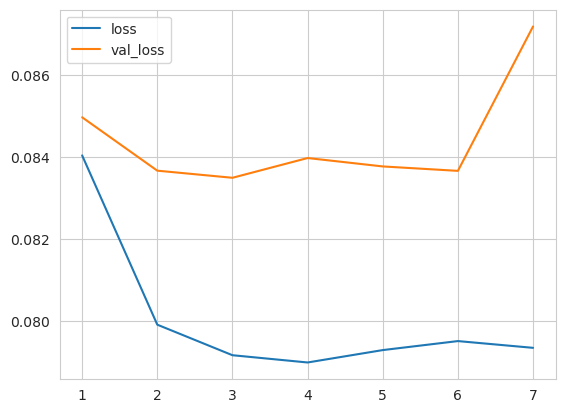
\includegraphics[width=\textwidth]{graphics/model_history_loss_clicks}
    \caption{Only clicks as features}
    \label{fig:model_history_loss_clicks}
  \end{subfigure}
  \hfill
  \begin{subfigure}[b]{0.45\textwidth}
    \centering
    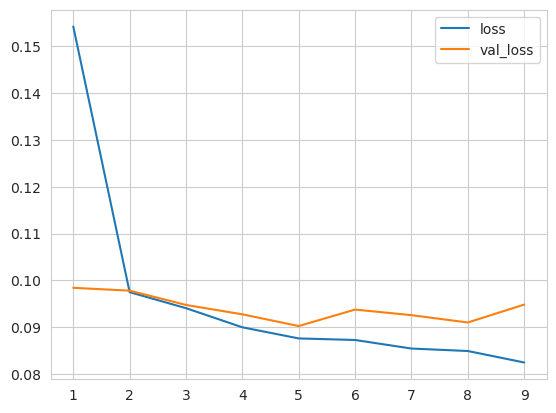
\includegraphics[width=\textwidth]{graphics/model_history_loss_features}
    \caption{Bounding box and click features}
    \label{fig:model_history_loss_features}
  \end{subfigure}
  \hfill
  \begin{subfigure}[b]{0.8\textwidth}
    \centering
    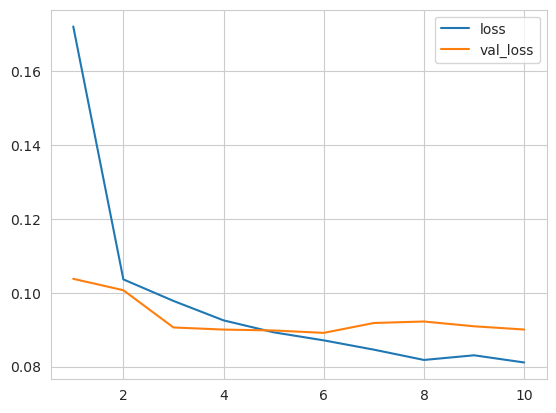
\includegraphics[width=\textwidth]{graphics/model_history_loss_features_shifted}
    \caption{Bounding box and shifted click features}
    \label{fig:model_history_loss_features_shifted}
  \end{subfigure}
  \caption[Training loss vs. validation loss]{Training loss (\ti{loss}, blue) vs. validation loss (\ti{val\_loss}, orange). Horizontal axis is the number of epochs. Vertical axis is the loss as \gls{mse}.}
  \label{fig:model_history_losses}
\end{figure}

\begin{table}[htbp!]
  \small
  \centering
  \begin{tabular}{|l|l|l|l|}
    \hline
    \textbf{Method}      & \textbf{Loss} & \textbf{Validation Loss} & \textbf{Number of epochs} \\
    \hline
    ClickOnly            & 0.0793        & 0.0872                   & 7                         \\
    SelectedFeatures     & 0.0824        & 0.0948                   & 9                         \\
    FeaturesClickShifted & 0.0811        & 0.0900                   & 10                        \\
    \hline
  \end{tabular}
  \caption[Training and validation loss, number of epochs]{Training and validation loss (\gls{mse}) of all three methods, ClickOnly, SelectedFeatures and FeaturesClickShifted}
  \label{tab:model_losses}
\end{table}

\todo{TAKEAWAY: click sequence may NOT a good indicator for where the user clicks, better relative actionable button click rate}

\section{Limitations}

Dataset
Dataset is not through different apps, only in one app.
Dataset is not detailed enough in the time steps, or not containing all data
Dataset is not long enough
Dataset has no paid apps or apps with login, which most services require
Dataset has wrong data see \cite{clay}

Preprocessing
Need more time to validate what are the core parameters to predict the next user intent


Model needs more investigation on what data is needed
How many neurons are required to achieve this
Play around with different layers, also Convolutional and pretrained embeddings

\todo{explain concept to help people, independently developed }


\chapter{Application of Android UI tree vectors}

\section{Automation and testing of Android apps}
\section{UI design similarities}
\section{Action prediction models, User behavior modeling}
\section{Behavioral analyses for smartphone usage patterns}


\section{What is a suitable model for the prediction of user intent?}.

To answer this question, LSTM has to be compared against other methods of predicting user intents.
As shown in \todo{add ref} classic stochastic approaches may can predict larger scope of the user such as the next app or a general user workflow.
But they are not sufficient for predicting views, screens, or even precise gesture inputs.
To overcome this limitation the \gls{ml}-models have established in large datasets.
As the described problem is to be contextualized in the prediction of time series, the following options are offered:
\begin{itemize}
    \item Simple \gls{rnn}
    \item \gls{gru}
    \item \gls{lstm}
    \item \gls{gl-transformer}
\end{itemize}

Simple \gls{rnn} is limited in the capacity of establishing long-term semantics.
\gls{gru} is missing the forget gate compared to the \gls{lstm} making it simpler and faster, but may perform weaker on complex datasets.
The \gls{gl-transformer} model has many advantages, such as fast and efficient training, parallelism of input sequences and recognizing long-term patterns through multi-head attention.
On the other hand few prior work was done in the mobile sector which covers prediction of \gls{ui} trees.
Therefore, no publicly available coding approach was found which could be extended.
Also, as described in~\cite{zhou2021large} the structure of the model is quite complex -- with two transformers -- and needs more processing steps in general.
\gls{lstm} is well documented and the common choice to predict time dependent series.
It is well-supported by Keras~(\ref{keras}) and easy to use.
Also, similar approaches have been made in the area of app prediction or app summarization~\ref{cite me}, which can be used as basis for this work, such as Screen2Words~\ref{subsec:screen2words}.


\section{At what level of detail the predictions can be made?}

As noted in the introduction the term \ti{intent} has a very wide scope.
It's prediction can only be made in fractions, or serve as indicator.
The semantically closest way and also the most detailed would be to describe the users intent in words, thus a description of what the user wants to do next.
Unfortunately, the users intent description cannot be determined yet, as no according dataset is provided.
An important step, the screen summarization as shown in Screen2words~\ref{subsec:screen2words}, already was made, which could also be fed with the users intention descriptions.
But this would then only reflect the already passed fulfilled intent and not the upcoming next purpose.
Also, the users flows can be predicted as shown in the works of ERICA~\ref{subsec:erica}.
Next app prediction already works quite well \ref{todo}, which also reflects the larger intent of the user, but is not very detailed.

In order to approximate that goal the assumption was made that the next user interaction also give hints on what the user is intending to achieve.
The interaction is resulting in another screen, which then the user (hopefully) intends to see.
So not only the interaction, but also the next contents, such as screen or single views can give a hint to the intent.
As it turns out, this is possible, if replacing the labels in the proposed model, but presumably it will not be very precise.

%category → app → screen → view → action
1. Predict Gestures, prediction of current screen, not next screen, is possible and can easily calculate distances between this and the next point
2. Predict Screen or parts of screens, labels not gestures, box positions, text prediction, decoded and compared to current output, more a qualitative evalutation,
3. Predict App -> Not possible with RICO, no cross app traces

\section{How the user can be supported with their tasks on didigal end devices?}


\chapter{Conclusion and Future Work}
\label{sec:zusfas}

\section*{Summary}
\section*{Outlook}

Future directions for research in this area

ChatGPT – Image Recognition – Limitation als Ausblick

Generate Dataset which overcomes the limitations

Make a study with actual feedback on a prediction system, visualization
-> Learn faster and directly, Reinforced learning

Work out user flows, like in ERICA, but without the need to separate it from the interaction tree

Take in visual and textual context (semantics).

Make dataset with app overlapping traces.
Use dataset with preprocessing such as RicoSCA or Clay.
Also use accessibility service, as phones are much more powerful.
No need for web interface.
-> Reinforced directly on the phone, more privacy.



\newpage
\todo{check if references are still on their own page}
\newpage
\printbibliography[heading=subbibliography]

%All links were last followed on March 17, 2018.

\appendix
% % !TeX root = main-english.tex
% !TeX spellcheck = en-US
% !TeX encoding = utf8
% -*- coding:utf-8 mod:LaTeX -*-

%This smart spell only works if no changes have been made to the chapter 
%using the options proposed in preambel/chapterheads.tex.
\setchapterpreamble[u]{%
  \dictum[Albert Einstein]{We cannot solve our problems with the same level of thinking that created them}
}
\chapter{LaTeX Hints}
\label{chap:latexhints}

One sentence per line.
This rule is important for the usage of version control systems.
A new line is generated with a blank line.
As you would do in Word:
New paragraphs are generated by pressing enter.
In LaTeX, this does not lead to a new paragraph as LaTeX joins subsequent lines.
In case you want a new paragraph, just press enter twice (!).
This leads to an empty line.
In word, there is the functionality to press shift and enter.
This leads to a hard line break.
The text starts at the beginning of a new line.
In LaTeX, you can do that by using two backslashes (\textbackslash\textbackslash).
This is rarely used.

Please do \textit{not} use two backslahes for new paragraphs.
For instance, this sentence belongs to the same paragraph, whereas the last one started a new one.
A long motivation for that is provided at \url{http://loopspace.mathforge.org/HowDidIDoThat/TeX/VCS/#section.3}.

One can write \emph{emphasized text (rendered in italics)} and \textbf{bold text}.

\section{File Encoding and Support of Umlauts}
\label{sec:firstsectioninlatexhints}
The template offers foll UTF-8 support.
All recent editors should not have issues with that.

\section{Citations}


References are set by means of \texttt{\textbackslash cite[key]}.

\begin{filecontents*}{\democodefile}
Example: \cite{WSPA} or by author input: \citet{WSPA}.
\end{filecontents*}
\PrintDemo{style=parallel}

The following sentence demonstrates
\begin{inparaenum}[1.]
  \item the capitalization of author names at the beginning of the sentence,
  \item the correct citation using author names and the reference,
  \item that the author names are a hyperlink to the bibliography and that
  \item the bibliography contains the name prefix \qq{van der} of \qq{Wil M.\,P.\ van der Aalst}.
\end{inparaenum}

\begin{filecontents*}{\democodefile}
\Citet{RVvdA2016} present a study on the effectiveness of workflow management systems.
\end{filecontents*}
\PrintDemo{style=parallel}

The following sentence demonstrates that you can overwrite the text part of the generated label using \texttt{label} in a bibliopgrahie"=entry, but the year and the uniqueness is still generated by biber.

\begin{filecontents*}{\democodefile}
The workflow engine Apache ODE \cite{ApacheODE} executes \BPEL processes reliably.
\end{filecontents*}
\PrintDemo{style=parallel}

\begin{filecontents*}{\democodefile}
Words are best enclosed using \texttt{\textbackslash qq\{..\}}, then the correct quotes are used.
\end{filecontents*}
\PrintDemo{style=parallel}

When creating the Bibtex file it is recommended to make sure that the DOI is listed.

\section{Formulas and Equations}
\label{sec:mf}

\begin{filecontents*}{\democodefile}
Equations $f(x)=x$ inside the text can be provided.
\end{filecontents*}
\PrintDemo{style=parallel}

A list with all available mathematical symbols is provided at \url{http://texdoc.net/pkg/symbols-a4}.

\begin{filecontents*}{\democodefile}
As example the set of natural numbers is given by $\mathbb{N}$.
\end{filecontents*}
\PrintDemo{style=parallel}

For the documentation of editing mathematical formulas read the package documentation of \texttt{amsmath}\footnote{\url{http://texdoc.net/pkg/amsmath}}.

Equation~\ref{eq:test} is numbered and can be referenced in the text:
\begin{filecontents*}{\democodefile}
\begin{align}
  \label{eq:test}
  x = y
\end{align}
\end{filecontents*}
\PrintDemo{style=parallel}

Following equation is not numbered because of using \texttt{\textbackslash align*} as environment.
\begin{filecontents*}{\democodefile}
\begin{align*}
  x = y
\end{align*}
\end{filecontents*}
\PrintDemo{style=parallel}

The template offers \verb+\abs+ to enable the bars scaling well at the absolute value:

\begin{filecontents*}{\democodefile}
$\abs{X}$.
\end{filecontents*}
\PrintDemo{style=parallel}

More details about mathematical environments provides the documentation available at \url{http://www.ctan.org/tex-archive/help/Catalogue/entries/voss-mathmode.html}.


%%%%%%%%%%%%%%%%%%%%%%%%%%%%%%%%%%%%%%%%%%%%%%%%%%%%%%%%%%%%%%%%%%%%%%%%%%%%%%
\section{Sourcecode}
%%%%%%%%%%%%%%%%%%%%%%%%%%%%%%%%%%%%%%%%%%%%%%%%%%%%%%%%%%%%%%%%%%%%%%%%%%%%%%
\autoref{lst:ListingANDlstlisting} shows how to emmbed source code.
With \texttt{\textbackslash lstinputlisting} the source code can be loaded directly from files.

%Listing-Umgebung wurde durch \newfloat{Listing} definiert
\begin{Listing}
  \begin{lstlisting}
<listing name="second sample">
  <content>not interesting</content>
</listing>
\end{lstlisting}
  \caption{The code is separated by two horizontal lines in the listings environment.}
  \label{lst:ListingANDlstlisting}
\end{Listing}

\begin{filecontents*}{\democodefile}
Source code is also available in the text \lstinline|<listing />|.
\end{filecontents*}
\PrintDemo{style=parallel}


%%%%%%%%%%%%%%%%%%%%%%%%%%%%%%%%%%%%%%%%%%%%%%%%%%%%%%%%%%%%%%%%%%%%%%%%%%%%%%
\section{Pseudocode}
%%%%%%%%%%%%%%%%%%%%%%%%%%%%%%%%%%%%%%%%%%%%%%%%%%%%%%%%%%%%%%%%%%%%%%%%%%%%%%
\autoref{alg:sample} shows a sample algorithm.
\begin{Algorithmus} %Use the environment only if you want to place the algorithm similar to graphics from TeX
  \caption{Sample algorithm}
  \label{alg:sample}
  \begin{algorithmic}
\Procedure{Sample}{$a$,$v_e$}
\State $\mathsf{parentHandled} \gets (a = \mathsf{process}) \lor \mathsf{visited}(a'), (a',c,a) \in \mathsf{HR}$
\State \Comment $(a',c'a) \in \mathsf{HR}$ denotes that $a'$ is the parent of $a$
\If{$\mathsf{parentHandled}\,\land(\mathcal{L}_\mathit{in}(a)=\emptyset\,\lor\,\forall l \in \mathcal{L}_\mathit{in}(a): \mathsf{visited}(l))$}
\State $\mathsf{visited}(a) \gets \text{true}$
\State $\mathsf{writes}_\circ(a,v_e) \gets
\begin{cases}
\mathsf{joinLinks}(a,v_e) & \abs{\mathcal{L}_\mathit{in}(a)} > 0\\
\mathsf{writes}_\circ(p,v_e)
& \exists p: (p,c,a) \in \mathsf{HR}\\
(\emptyset, \emptyset, \emptyset, false) & \text{otherwise}
\end{cases}
$
\If{$a\in\mathcal{A}_\mathit{basic}$}
  \State \Call{HandleBasicActivity}{$a$,$v_e$}
\ElsIf{$a\in\mathcal{A}_\mathit{flow}$}
  \State \Call{HandleFlow}{$a$,$v_e$}
\ElsIf{$a = \mathsf{process}$} \Comment Directly handle the contained activity
  \State \Call{HandleActivity}{$a'$,$v_e$}, $(a,\bot,a') \in \mathsf{HR}$
  \State $\mathsf{writes}_\bullet(a) \gets \mathsf{writes}_\bullet(a')$
\EndIf
\ForAll{$l \in \mathcal{L}_\mathit{out}(a)$}
  \State \Call{HandleLink}{$l$,$v_e$}
\EndFor
\EndIf
\EndProcedure
  \end{algorithmic}
\end{Algorithmus}

\clearpage
And if you want to write an algorithm that goes over several pages, you can only do this with the following \textbf{dirty} hack:

{
\begin{minipage}{\textwidth}
  \hrule height .8pt width\textwidth
  \vskip.3em%\vskip\abovecaptionskip\relax
  \stepcounter{Algorithmus}
  \addcontentsline{alg}{Algorithmus}{\protect\numberline{\theAlgorithmus}{\ignorespaces Description \relax}}
  \noindent\textbf{Algorithmus \theAlgorithmus} Description
  %\stepcounter{algorithm}
  %\addcontentsline{alg}{Algorithmus}{\thealgorithm{}\hskip0em Description}
  %\textbf{Algorithmus \thealgorithm} Description
  \vskip.3em%\vskip\belowcaptionskip\relax
  \hrule height .5pt width\textwidth
\end{minipage}
%without the following line, the text is nerer at the rule
\vskip-.3em
%
code goes here\\
test2\\
%
\vskip-.7em
\hrule height .5pt width\textwidth
}


%%%%%%%%%%%%%%%%%%%%%%%%%%%%%%%%%%%%%%%%%%%%%%%%%%%%%%%%%%%%%%%%%%%%%%%%%%%%%%
\section{Figures}
%%%%%%%%%%%%%%%%%%%%%%%%%%%%%%%%%%%%%%%%%%%%%%%%%%%%%%%%%%%%%%%%%%%%%%%%%%%%%%
The \autoref{fig:chor1} and \ref{fig:chor2} are important to understand this document.
In the appendix \vref{fig:AnhangsChor} shows again the complete choreography.

%The parameters in square brackets are optional - e.g. [htb!]
%htb! means: Dear LaTeX, please place this image here first ("_h_ere"). If this does not work, place it at the "_t_op" of the page. And if this is not possible, please place it at the "_b_ottom" of the page. And please, please prefer here and above, even if it doesn't look so optimal ("!")
%These should NOT be used if possible. LaTeX's algorithm for placing the glide environment is already very good!
\begin{figure}
  \centering
  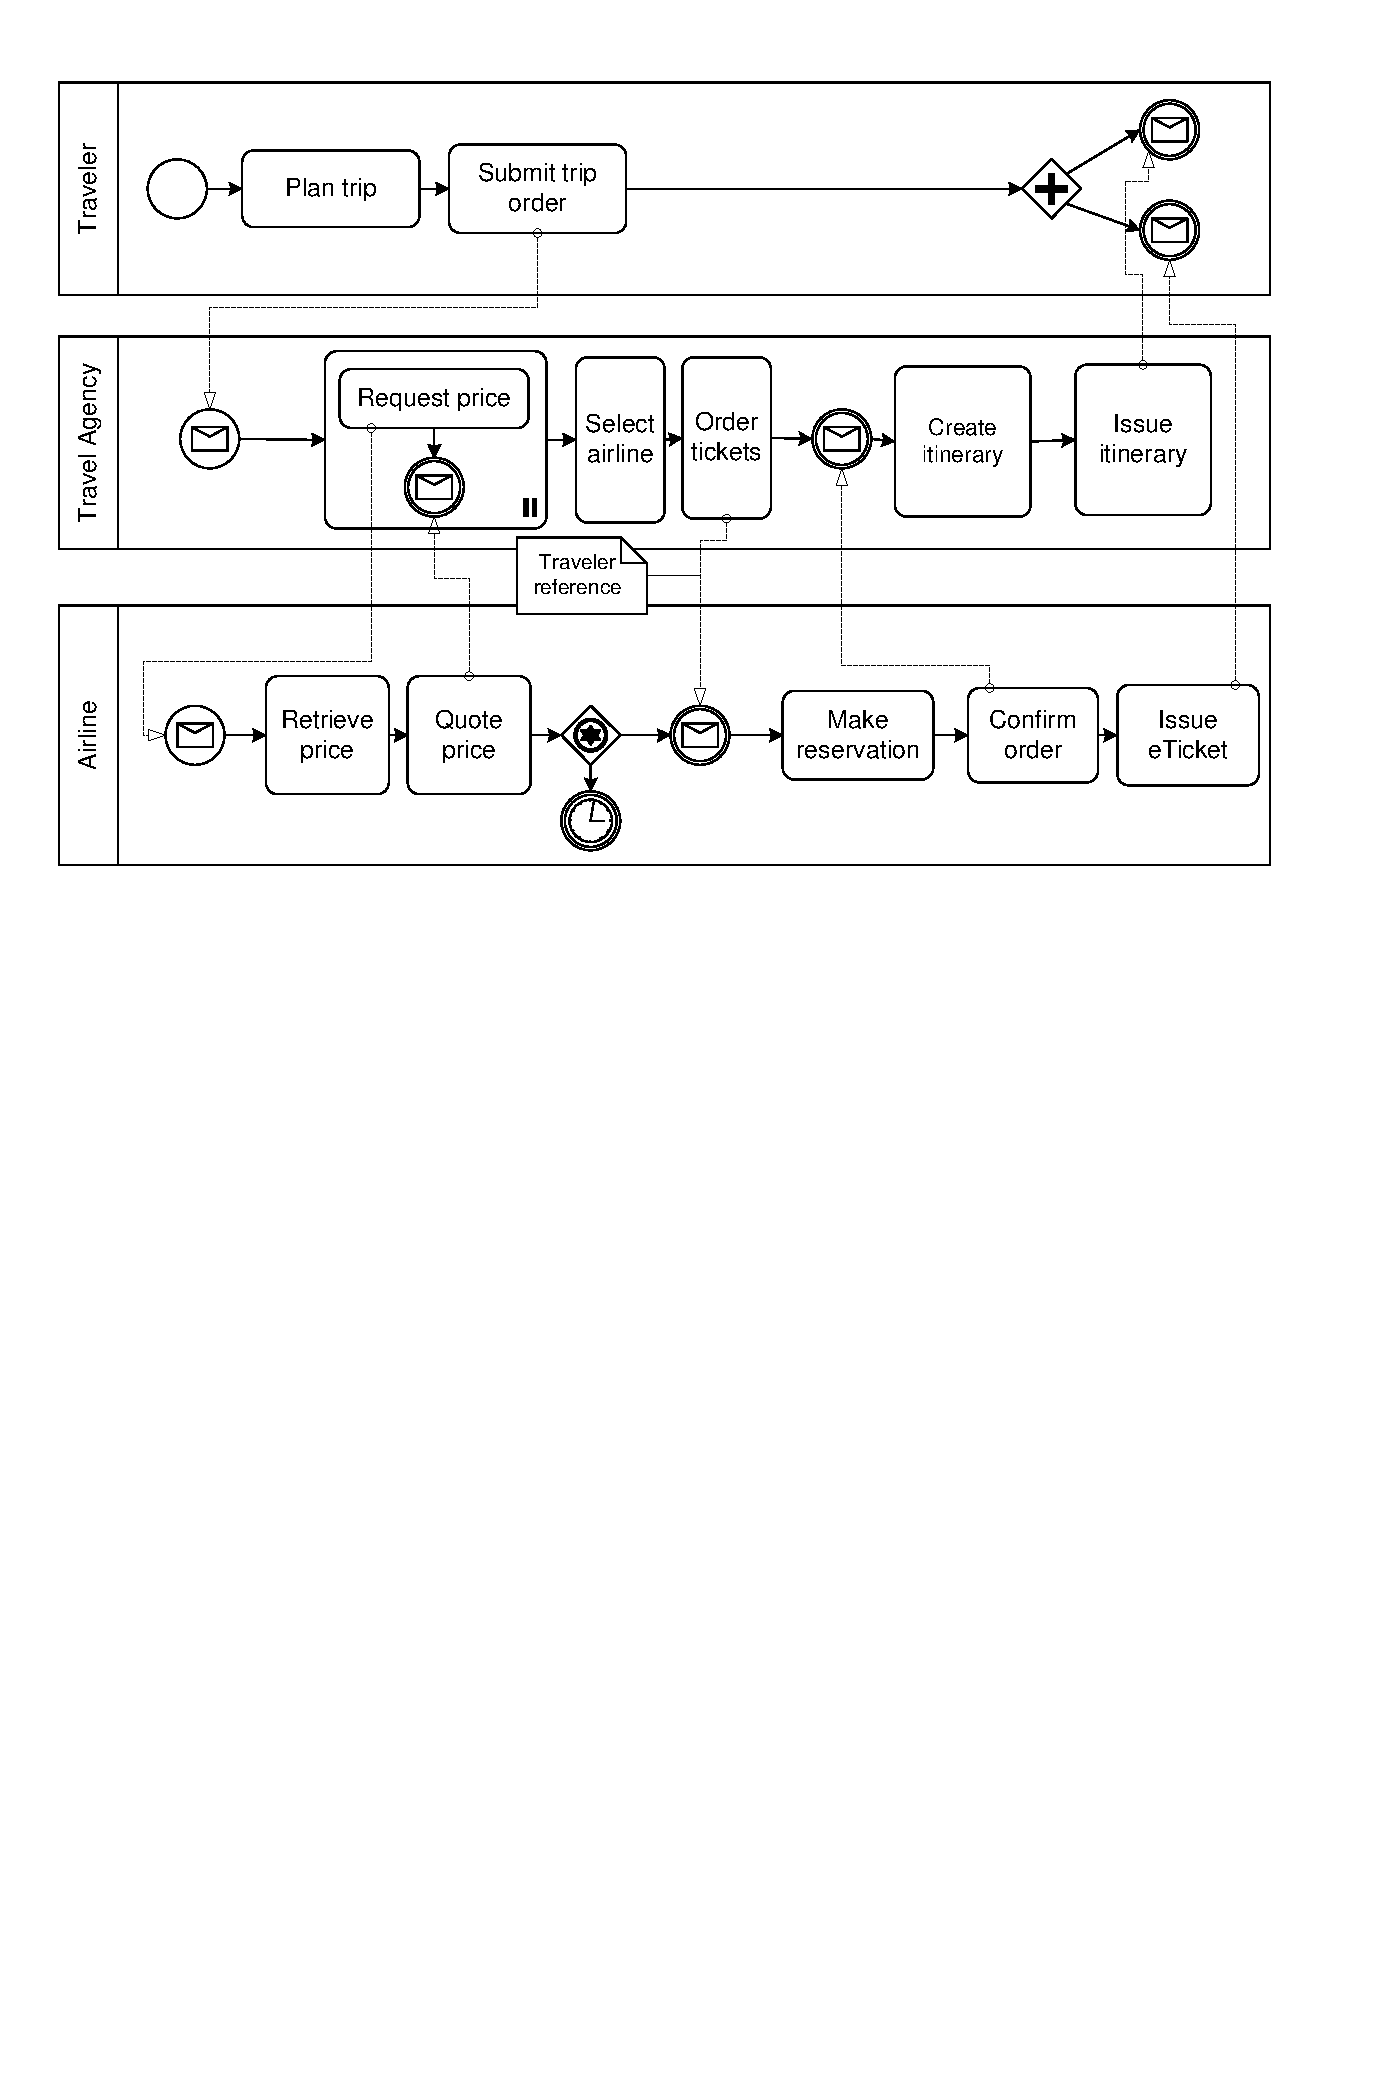
\includegraphics[width=\textwidth]{choreography.pdf}
  \caption{Example Choreography}
  \label{fig:chor1}
\end{figure}

\begin{figure}
  \centering
  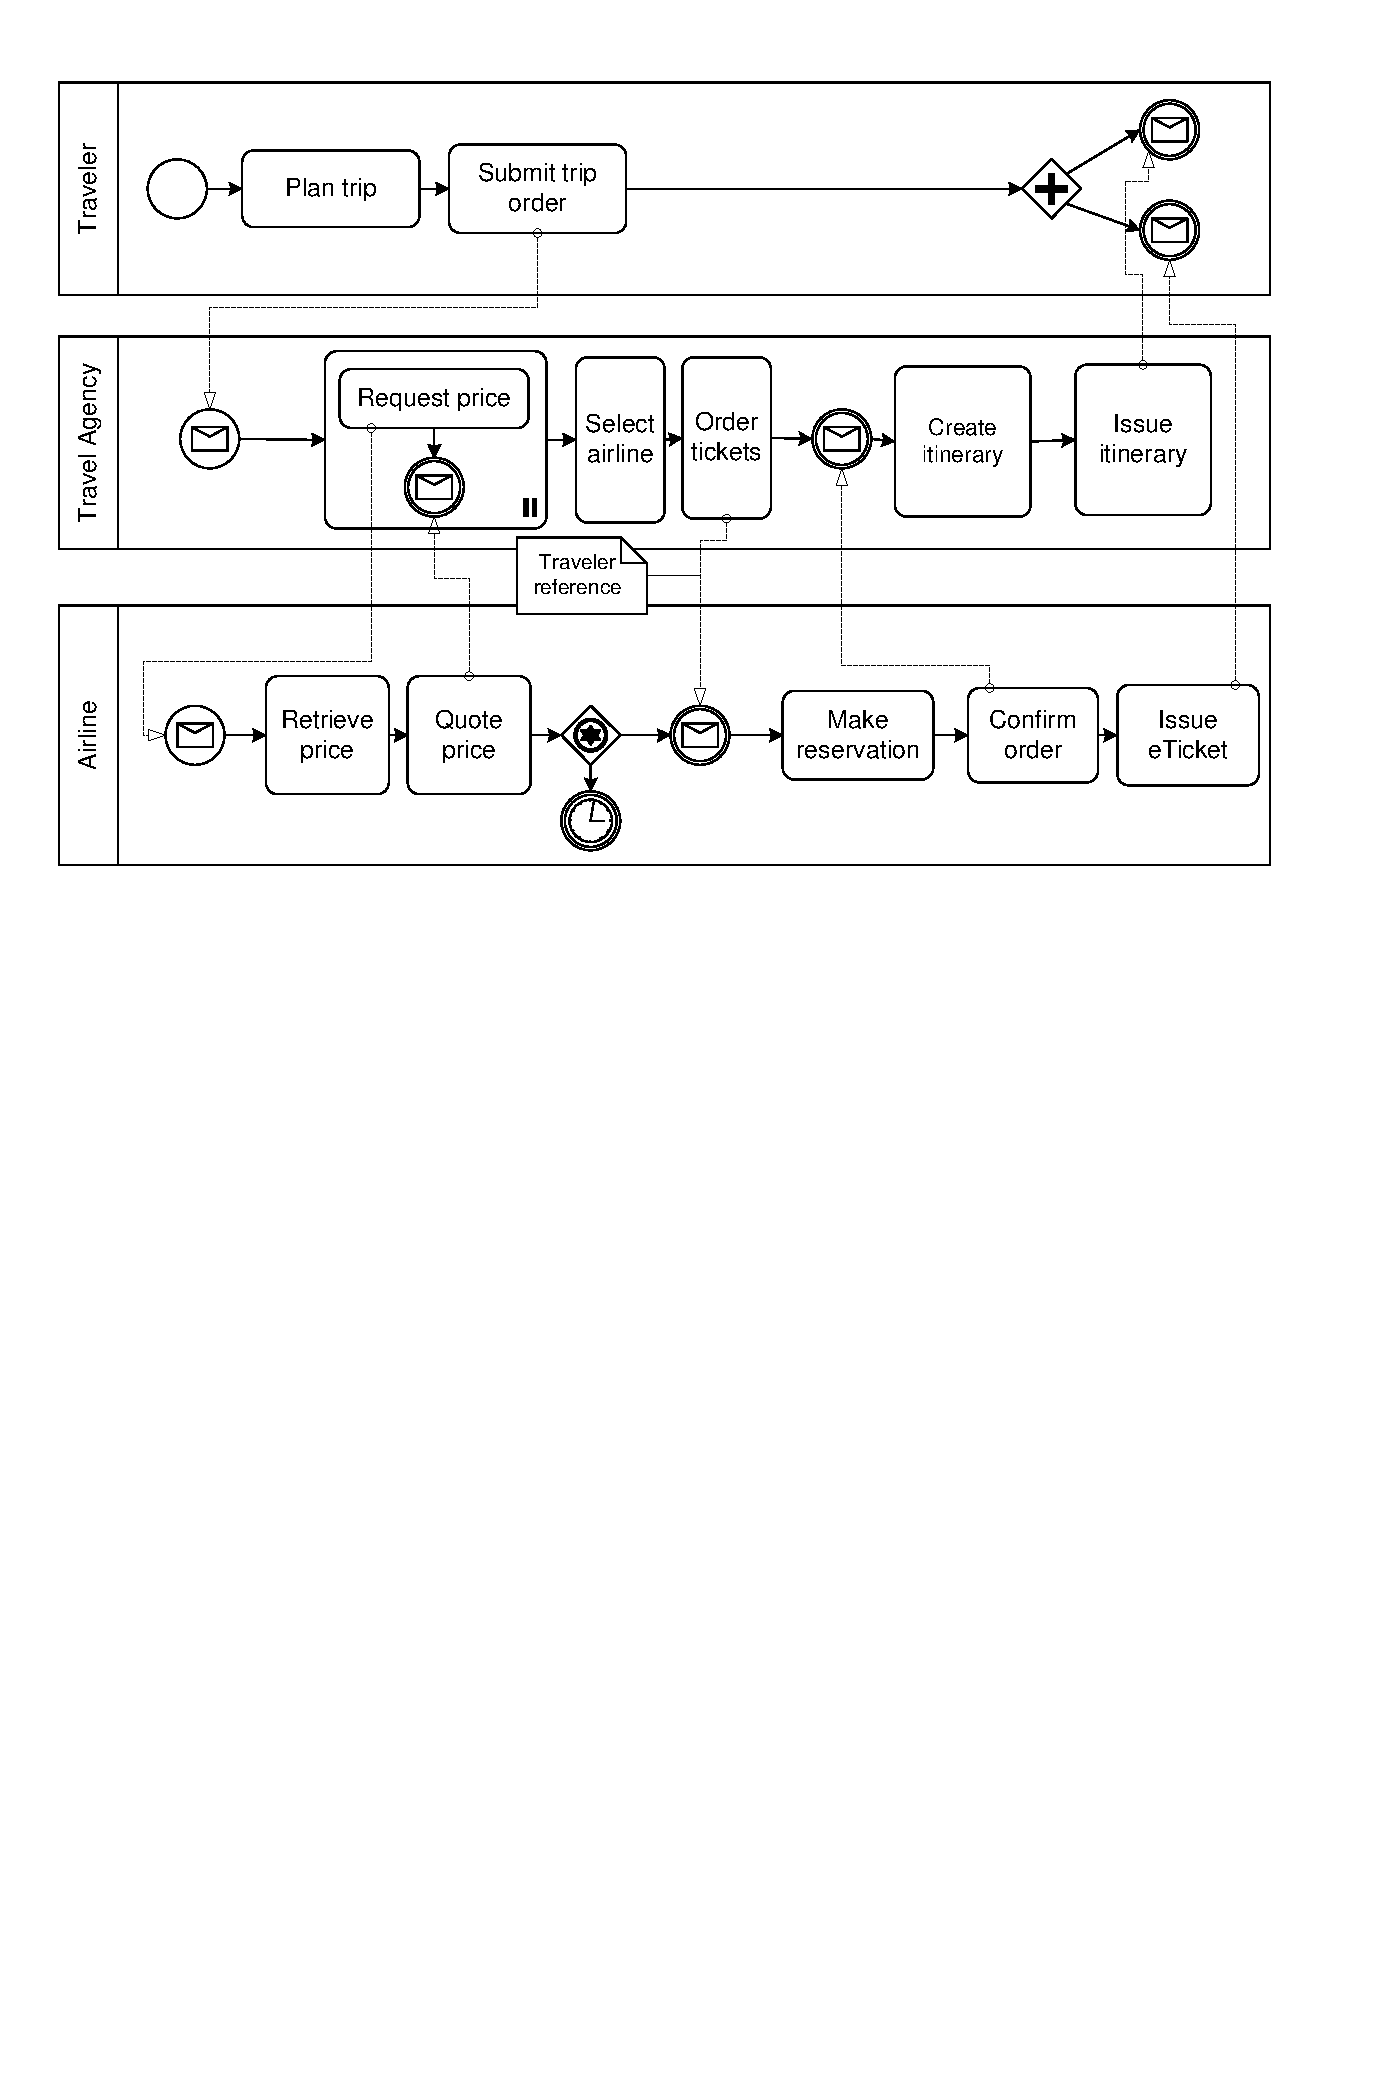
\includegraphics[width=.8\textwidth]{choreography.pdf}
  \caption[Example Choreography]{The example choreography. Now slightly smaller to demonstrate \texttt{\textbackslash textwidth}. And also the use of alternative captions for the list of images. However, the latter is only conditionally recommended, because who reads so much text under a picture? Or is it just a matter of style?}
  \label{fig:chor2}
\end{figure}


\begin{figure}
  \hfill
  \begin{subfigure}{.3\textwidth}
    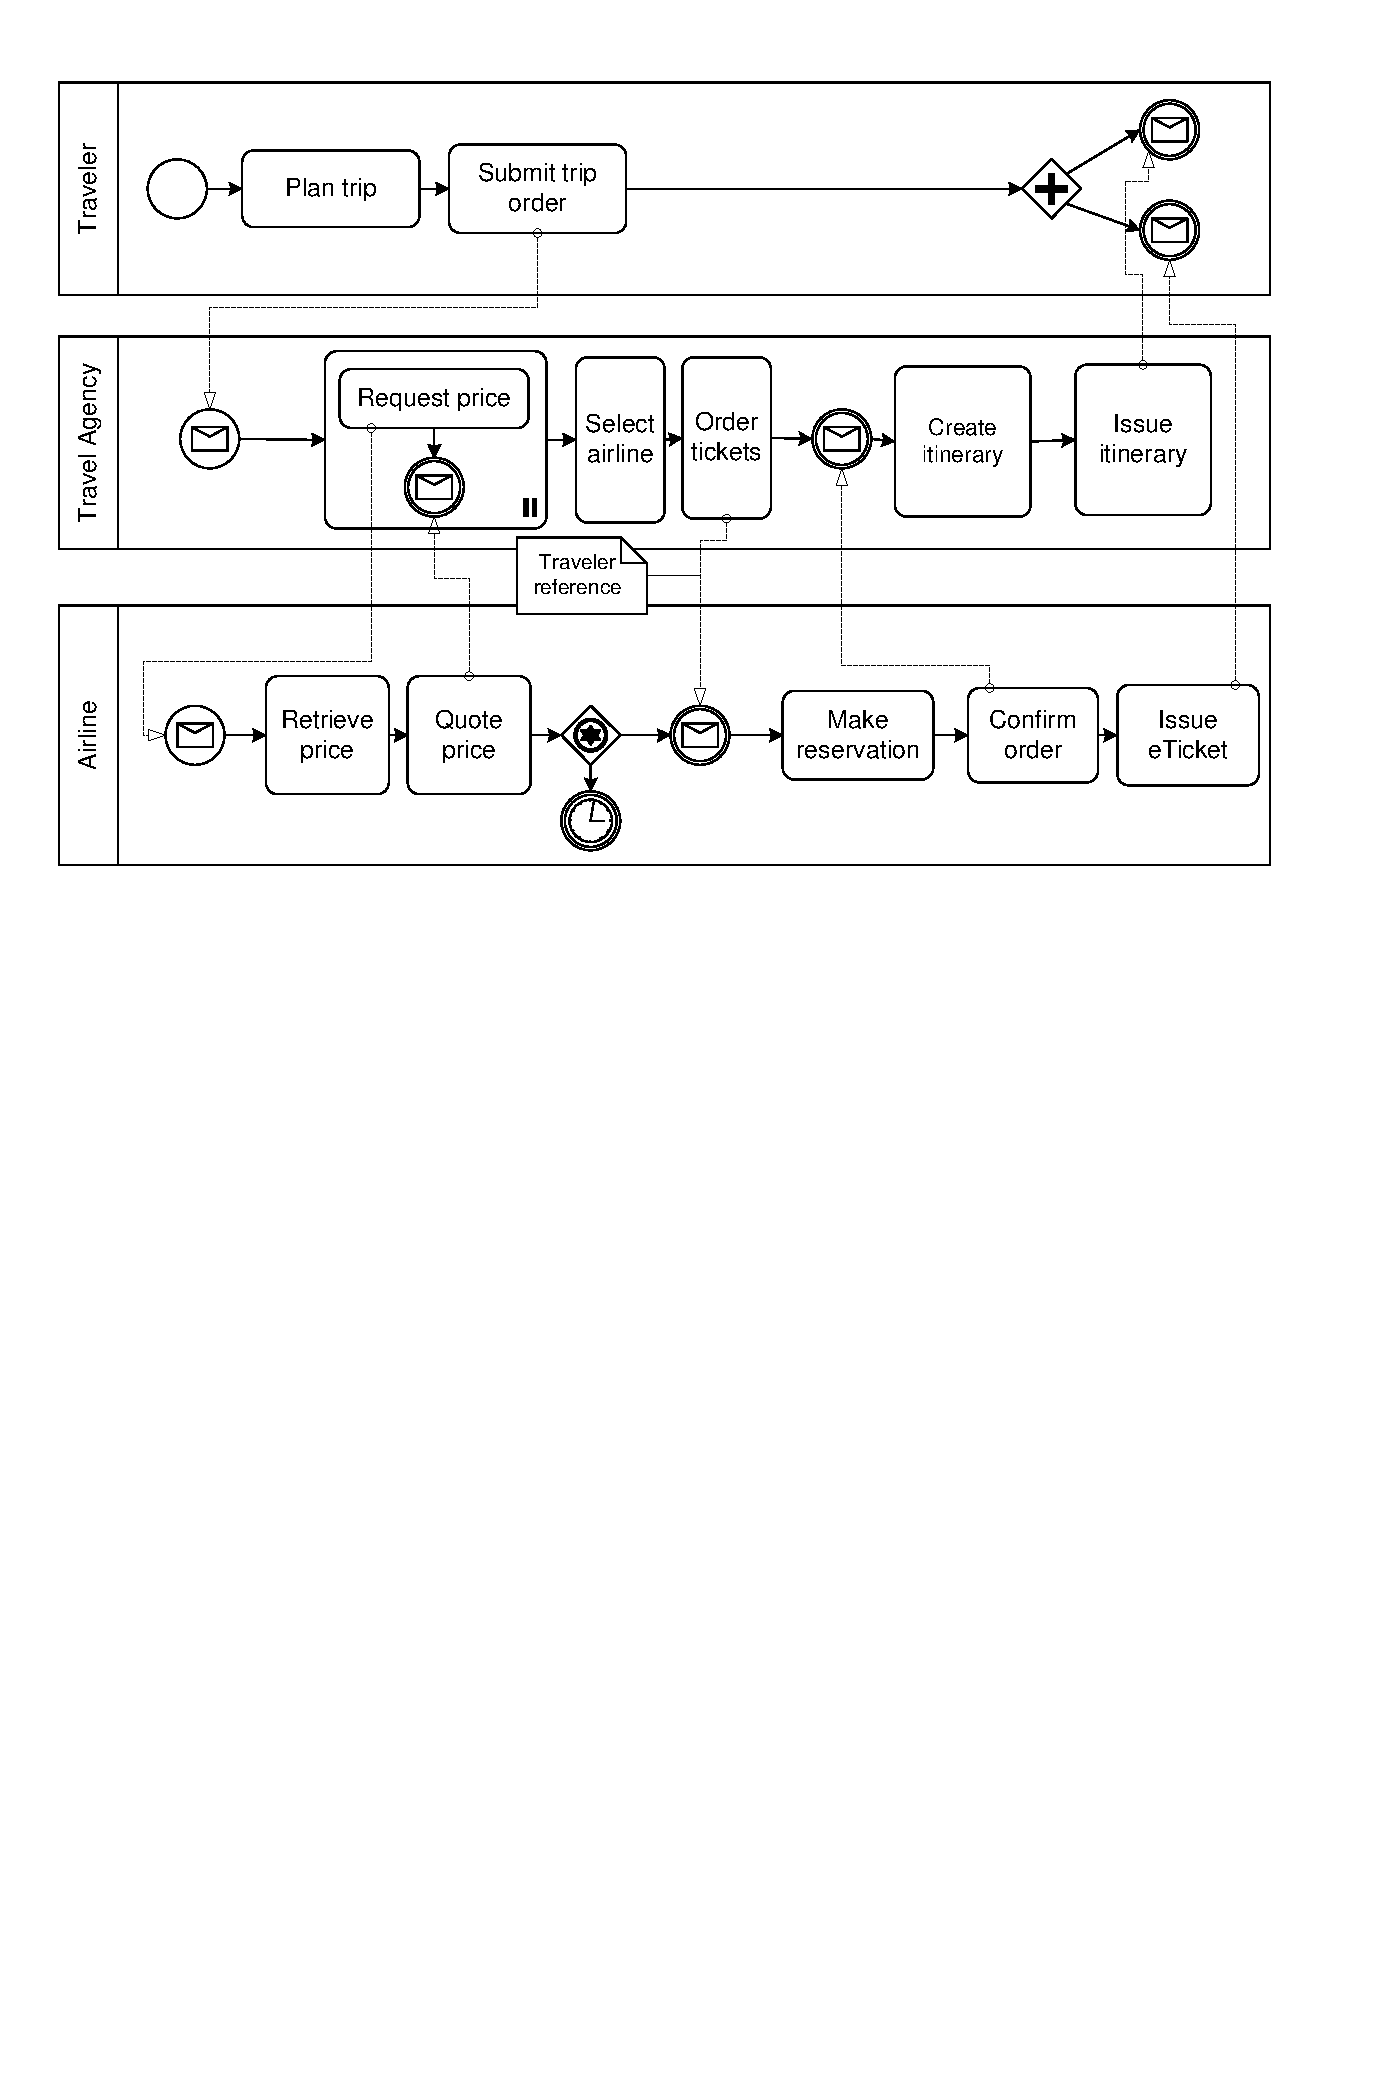
\includegraphics[width=\textwidth]{choreography.pdf}
    \caption{Choreography 1}
    \label{fig:subfigA}
  \end{subfigure}
  \hfill
  \begin{subfigure}{.3\textwidth}
    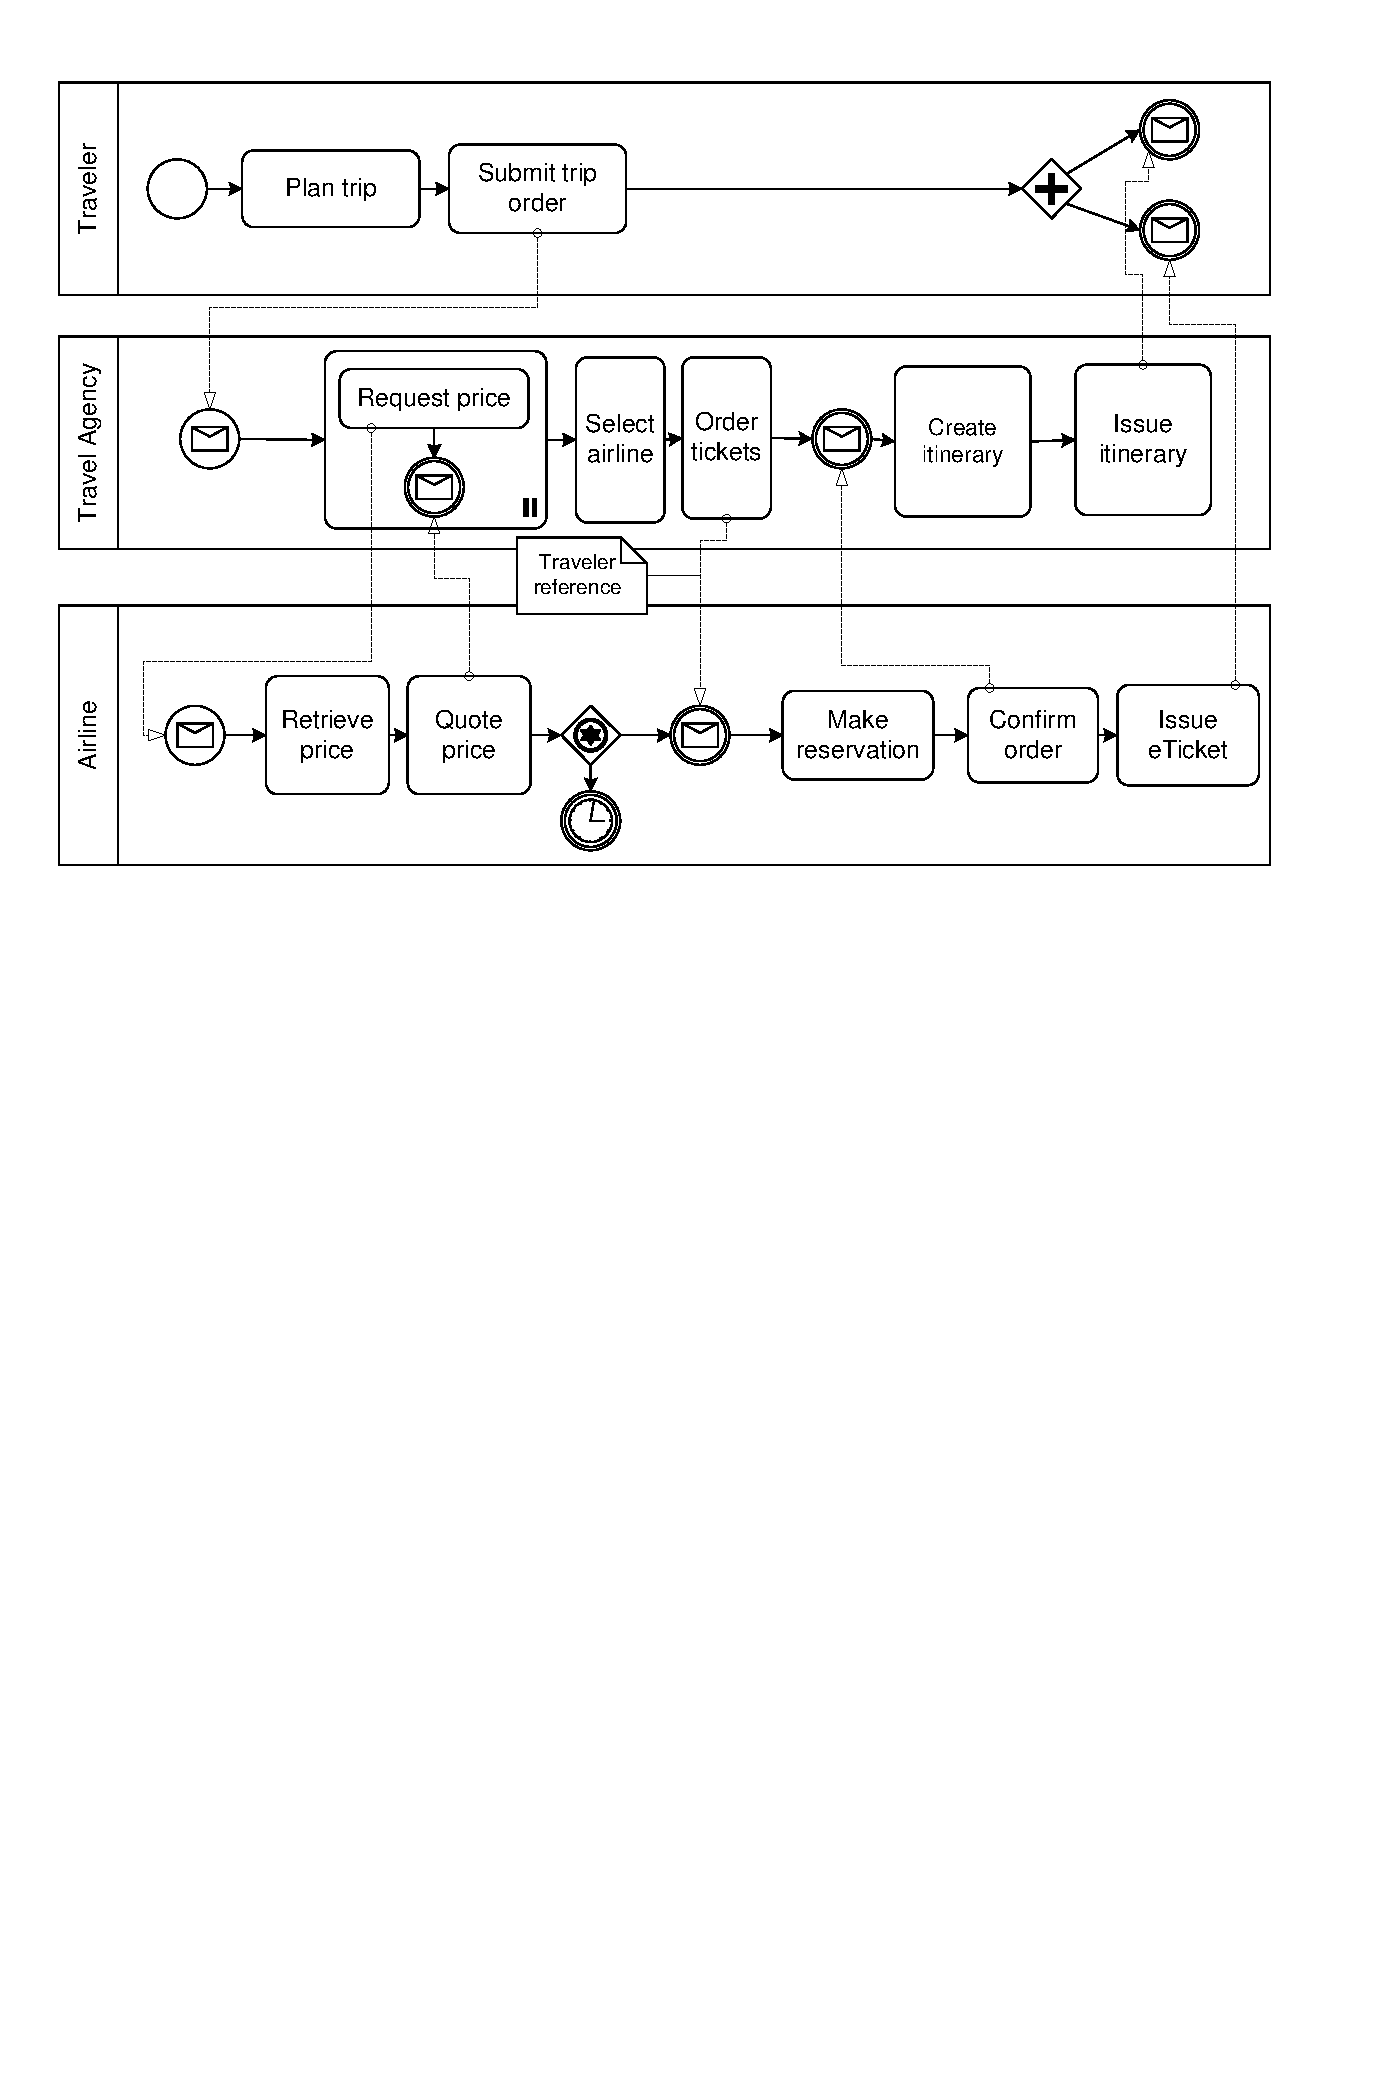
\includegraphics[width=\textwidth]{choreography.pdf}
    \caption{Choreography 2}
    \label{fig:subfigB}
  \end{subfigure}
  \hfill
  \begin{subfigure}{.3\textwidth}
    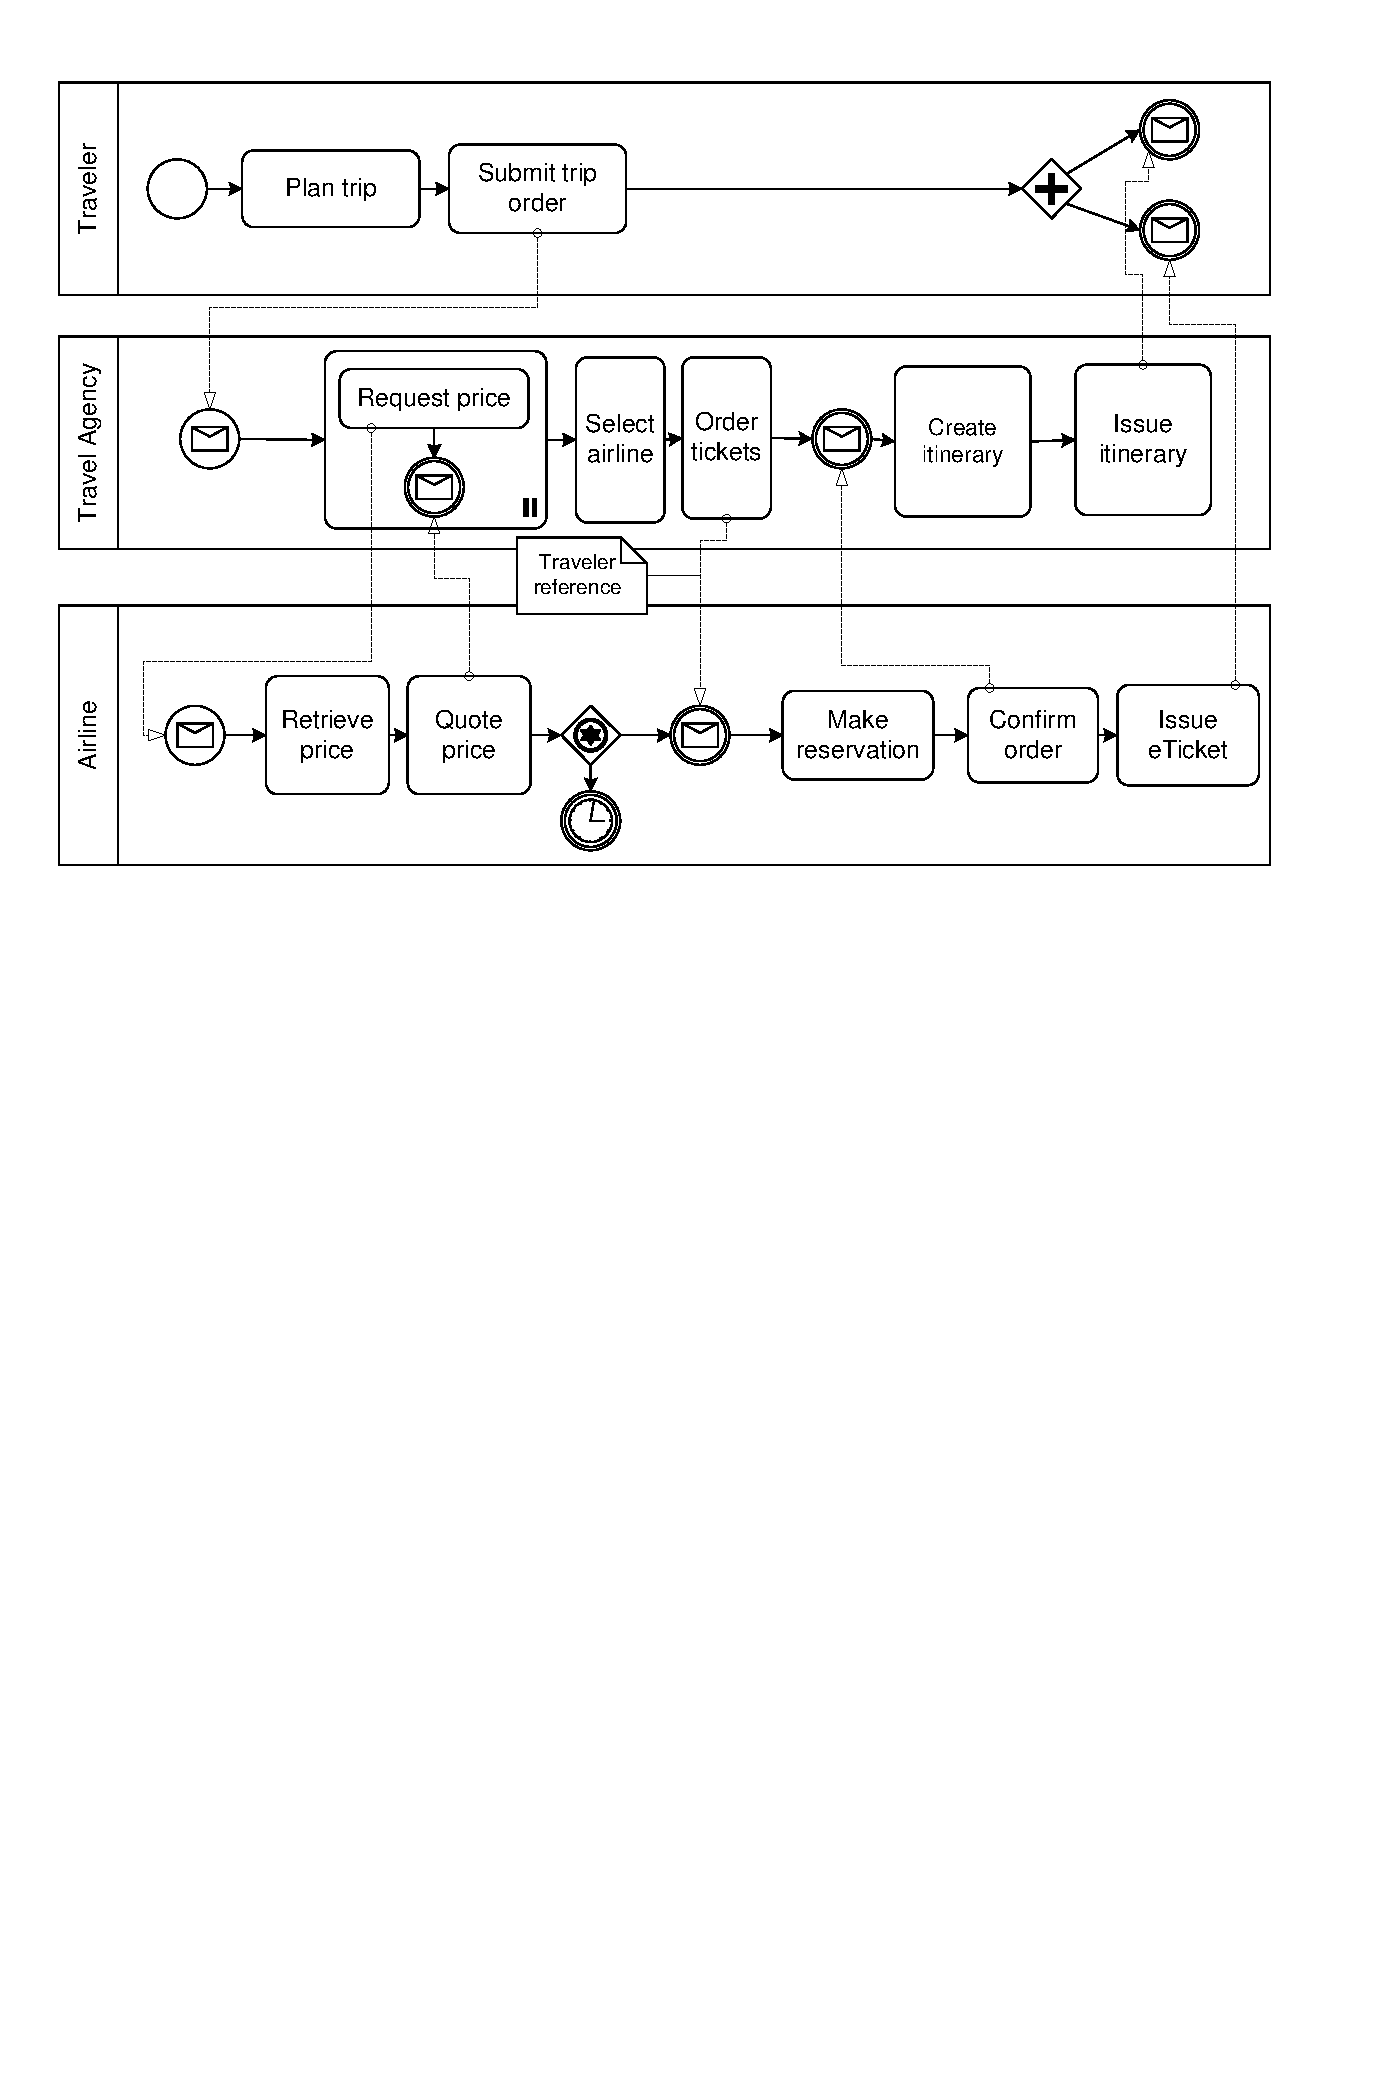
\includegraphics[width=.9\textwidth]{choreography.pdf}
    \caption{Choreography 3}
    \label{fig:subfigC}
  \end{subfigure}
  \caption{Example to place 3 illustrations next to each other. Further, it is possible to reference each separately.}
  \label{fig:subfig_example}
\end{figure}

\autoref{fig:subfig_example} shows the usage of the package subcaption.
It is indeed possible to reference to sub figures: \autoref{fig:subfigA}.

It is possible to convert SVGs to PDF directly during compilation.
This is described in the source code of latex-tipps.tex, but commented out.

\iffalse % <-- Take this away if inkscape is in the path
  The SVG in \autoref{fig:directSVG} is directly included, while the text in the SVG in \autoref{fig:latexSVG} is set using pdflatex.
  If you want to see the graphics, inkscape must be in PATH and in the text source \texttt{\textbackslash{}iffalse} and \text{\textbackslash{}iftrue} have to be commented out.

  \begin{figure}
    \centering
    
\includegraphics{svgexample.svg}
    \caption{SVG directly included}
    \label{fig:directSVG}
  \end{figure}

  \begin{figure}
    \centering
    \def\svgwidth{.4\textwidth}
    \includesvg{svgexample}
    \caption{Text in SVN set via \LaTeX{}}
    \label{fig:latexSVG}
  \end{figure}
\fi % <-- Take this away if inkscape is in the path



\section{More Illustrations}
\autoref{fig:AnhangsChor,fig:AnhangsChor2} show two choreographies, which should further explain the facts. The second figure is rotated 90 degrees to demonstrate the \texttt{pdflscape} package.

\begin{figure}
  \centering
  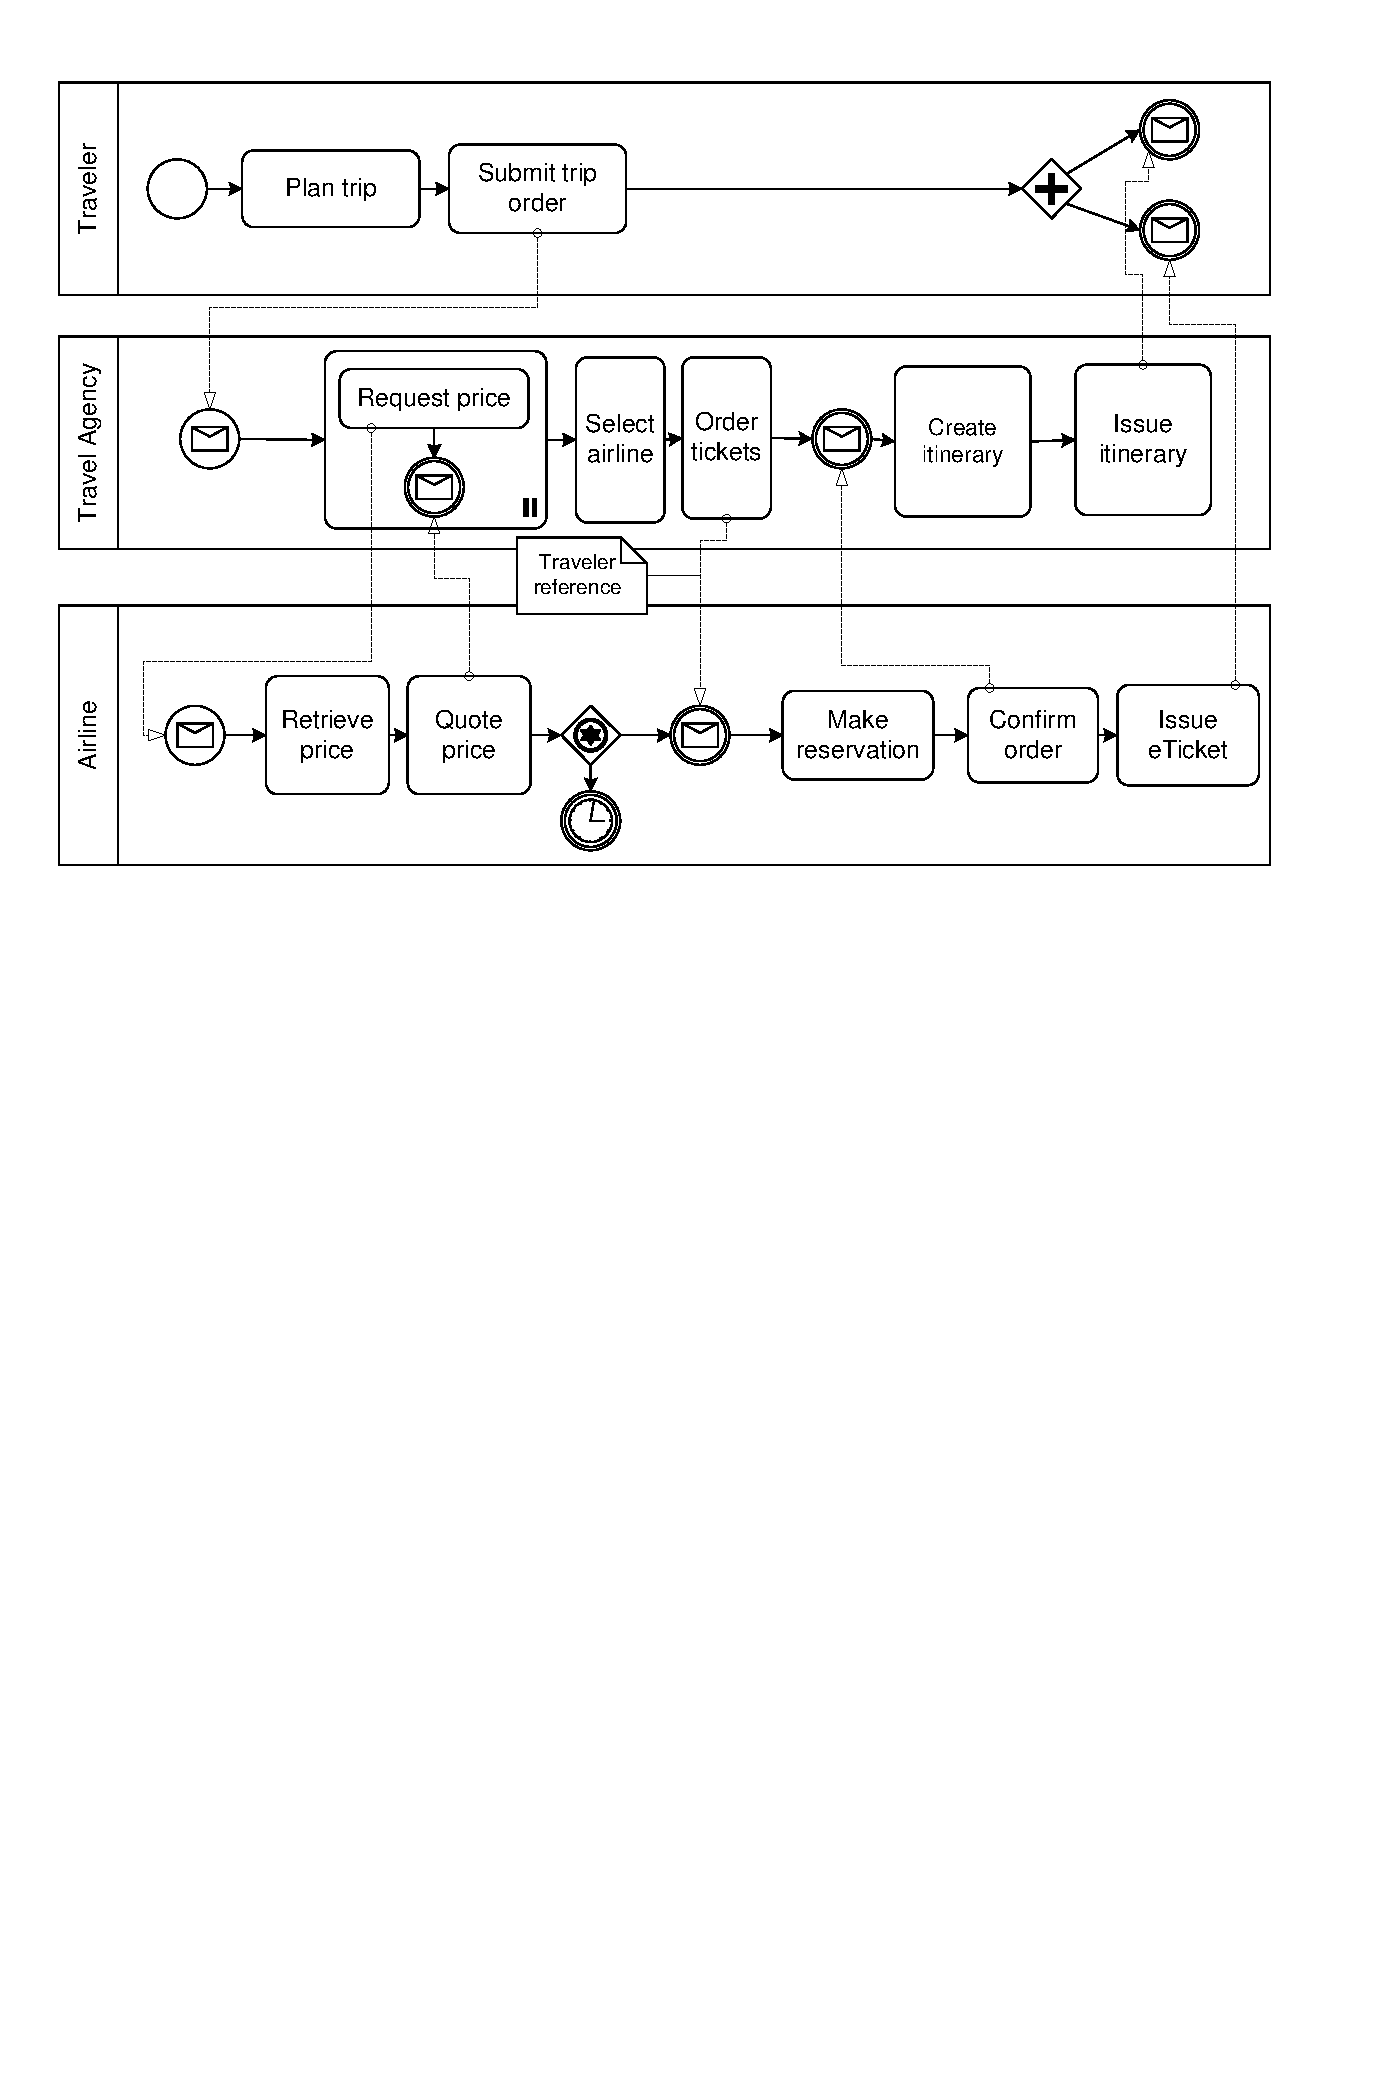
\includegraphics[width=\textwidth]{choreography.pdf}
  \caption{Example Choreography I}
  \label{fig:AnhangsChor}
\end{figure}

\begin{landscape}
  %sidewaysfigure
  \begin{figure}
    \centering
    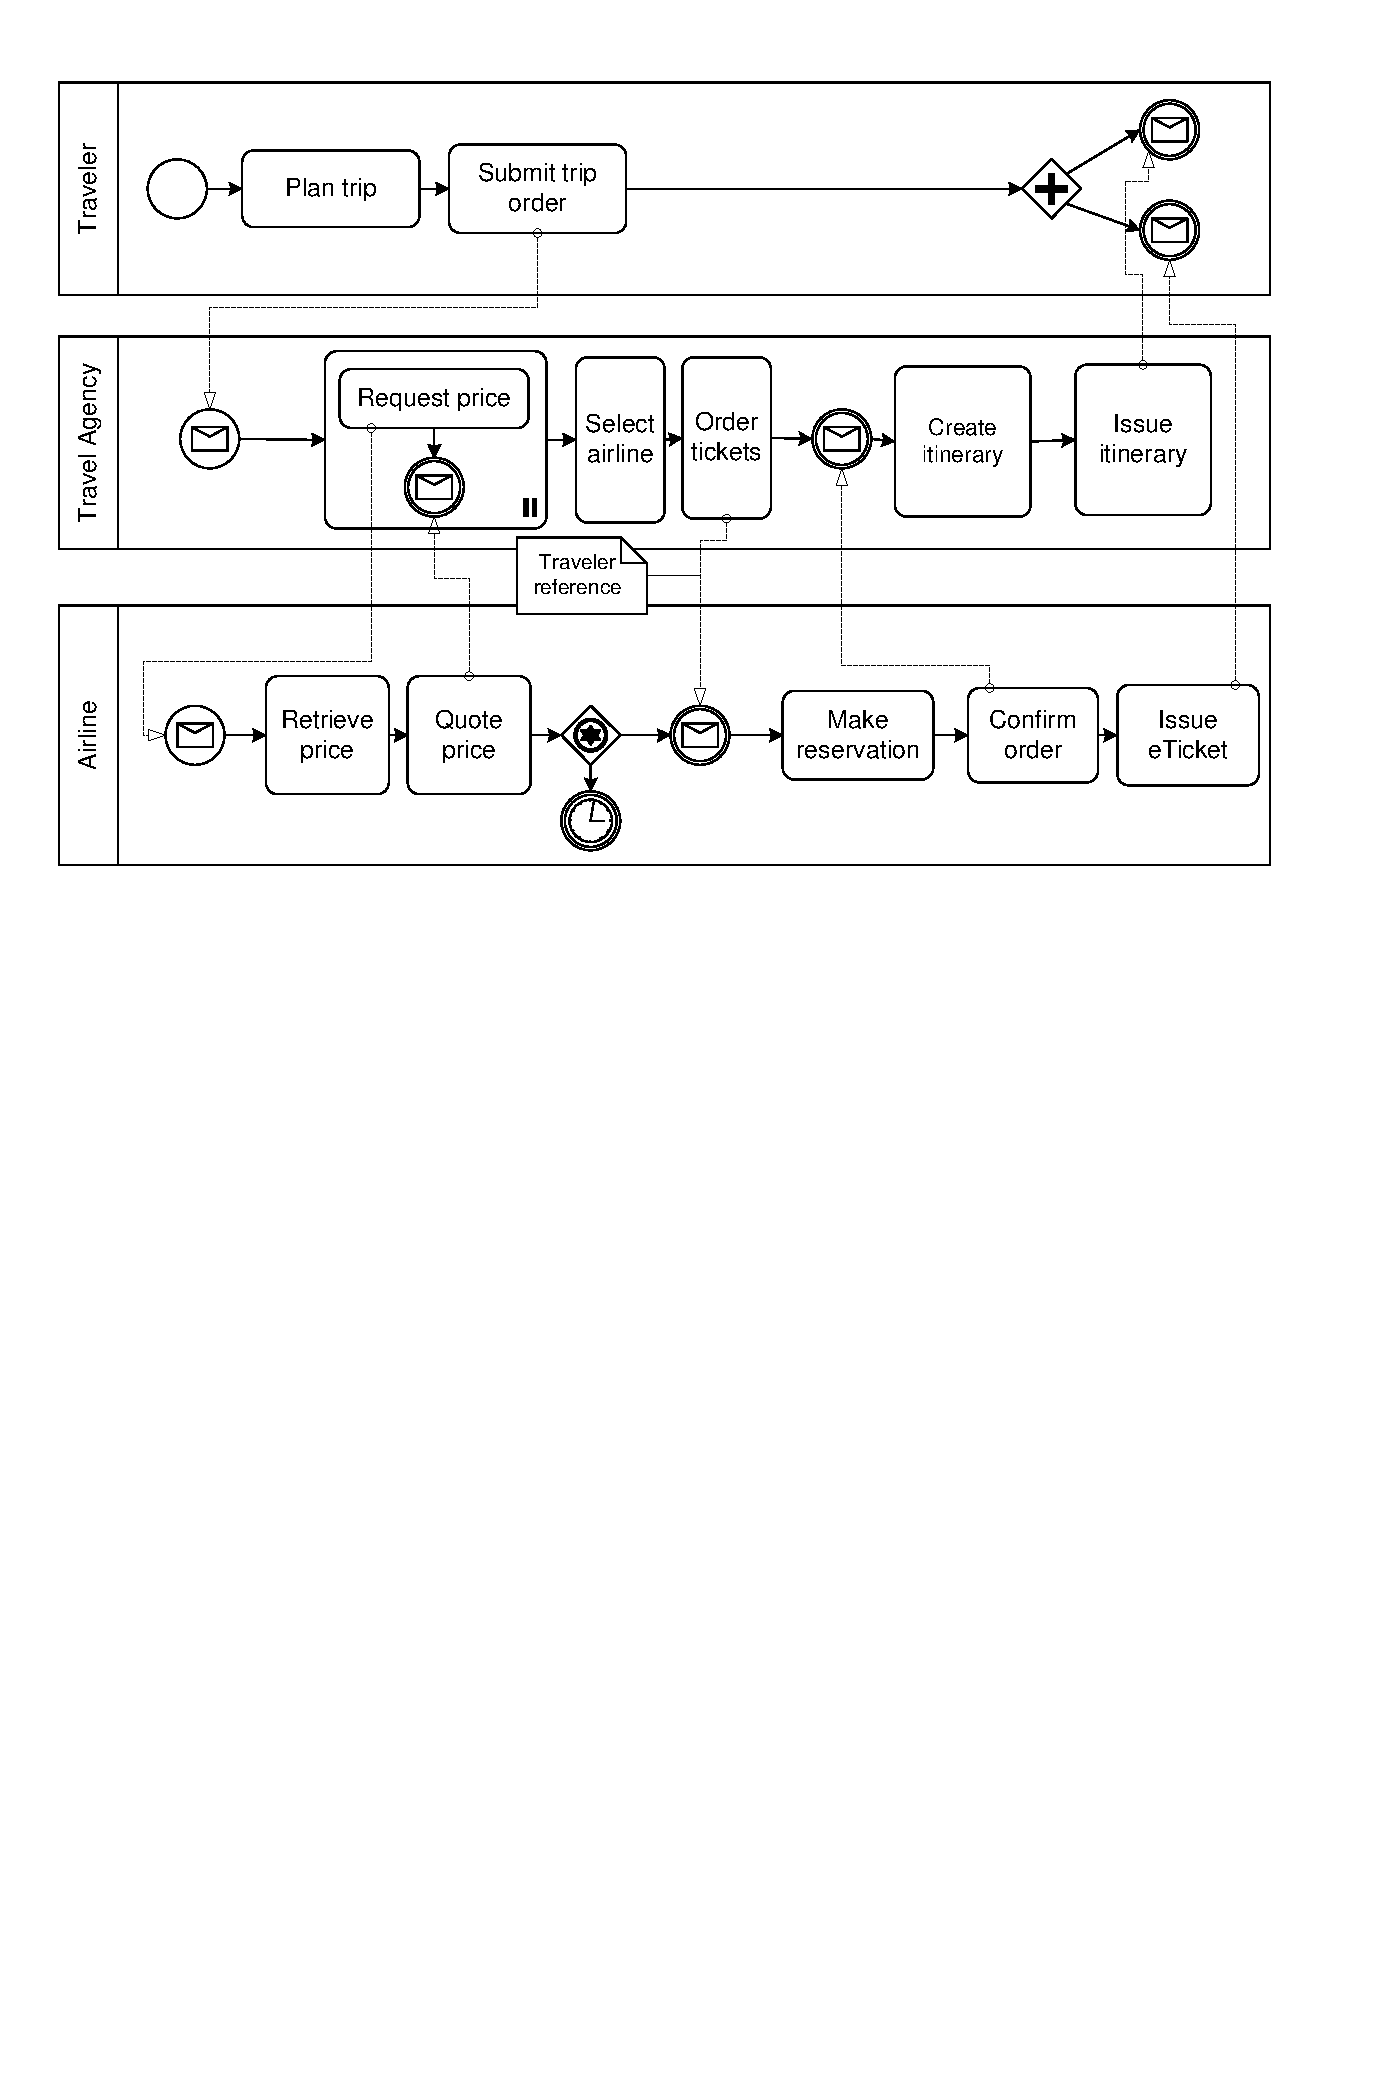
\includegraphics[width=\textwidth]{choreography.pdf}
    \caption{Example Choreography II}
    \label{fig:AnhangsChor2}
  \end{figure}
\end{landscape}


\IfFileExists{pgfplots.sty}{
  %%%%%%%%%%%%%%%%%%%%%%%%%%%%%%%%%%%%%%%%%%%%%%%%%%%%%%%%%%%%%%%%%%%%%%%%%%%%%%
  \section{Plots with pgfplots}
  %%%%%%%%%%%%%%%%%%%%%%%%%%%%%%%%%%%%%%%%%%%%%%%%%%%%%%%%%%%%%%%%%%%%%%%%%%%%%%
  The package pdfplots provides plotting of functions directly in \LaTeX~like with matlab or gnuplot. Some visual examples are available here\footnote{\url{http://texdoc.net/pkg/visualtikz}}.
  \begin{figure}[h]
    \centering
    \begin{tikzpicture}
      \begin{axis}[xlabel=$x$,
          ylabel=$\sin(x)$]
        \addplot {sin(deg(x))};  % Print sine function
      \end{axis}
    \end{tikzpicture}
    \caption{Plot of $\sin(x)$ direclty inside the figure environment with pgfplots.}
  \end{figure}

  \begin{figure}[h]
    \centering
    \begin{tikzpicture}
      \begin{axis}[xlabel=$x$,
          ylabel=$y$]
        \addplot table [x=a, y=c, col sep=comma] {data/data.csv};  % Read coordinates from csv file and plot them
      \end{axis}
    \end{tikzpicture}
    \caption{Coordinates $x$ and $y$ read from csv file and plotted pgfplots.}
  \end{figure}

}{}


%%%%%%%%%%%%%%%%%%%%%%%%%%%%%%%%%%%%%%%%%%%%%%%%%%%%%%%%%%%%%%%%%%%%%%%%%%%%%%
\section{Figures with tikz}
%%%%%%%%%%%%%%%%%%%%%%%%%%%%%%%%%%%%%%%%%%%%%%%%%%%%%%%%%%%%%%%%%%%%%%%%%%%%%%
The tikz is a package for creating graphics programmatically. With this package grids or other regular strucutres can be easliy generated.

\begin{figure}[ht]
  \centering
  \begin{tikzpicture}
    \draw(0,0) rectangle (4,4);
    \foreach \x in {0.5,1,1.5,2,2.5,3,3.5}
    \foreach \y in {0.5,1,1.5,2,2.5,3,3.5}
    \draw(\x,\y) circle (1pt);
  \end{tikzpicture}
  \caption{A regular grid genrated with easily with two for loops.}\label{fig:tikz_example}
\end{figure}


%%%%%%%%%%%%%%%%%%%%%%%%%%%%%%%%%%%%%%%%%%%%%%%%%%%%%%%%%%%%%%%%%%%%%%%%%%%%%%
\section{UML diagrams using tikz-uml}
%%%%%%%%%%%%%%%%%%%%%%%%%%%%%%%%%%%%%%%%%%%%%%%%%%%%%%%%%%%%%%%%%%%%%%%%%%%%%%

\autoref{fig:uml} presents a class diagram typeset using tikz-uml.

\begin{figure}
  \centering
  \begin{tikzpicture}
  \begin{umlpackage}{p}
  \begin{umlpackage}{sp1}
  \umlclass[template=T]{A}{
    n : uint \\ t : float
  }{}
  \umlclass[y=-3]{B}{
    d : double
  }{
    \umlvirt{setB(b : B) : void} \\ getB() : B}
  \end{umlpackage}
  \begin{umlpackage}[x=10,y=-6]{sp2}
  \umlinterface{C}{
    n : uint \\ s : string
  }{}
  \end{umlpackage}
  \umlclass[x=2,y=-10]{D}{
    n : uint
    }{}
  \end{umlpackage}

  \umlassoc[geometry=-|-, arg1=tata, mult1=*, pos1=0.3, arg2=toto, mult2=1, pos2=2.9, align2=left]{C}{B}
  \umlunicompo[geometry=-|, arg=titi, mult=*, pos=1.7, stereo=vector]{D}{C}
  \umlimport[geometry=|-, anchors=90 and 50, name=import]{sp2}{sp1}
  \umlaggreg[arg=tutu, mult=1, pos=0.8, angle1=30, angle2=60, loopsize=2cm]{D}{D}
  \umlinherit[geometry=-|]{D}{B}
  \umlnote[x=2.5,y=-6, width=3cm]{B}{A note with respect to class B}
  \umlnote[x=7.5,y=-2]{import-2}{A anotation}
  \end{tikzpicture}
  \caption{Class diagram generated with tikz-uml. Example adapted from Nicolas Kielbasiewicz.}
  \label{fig:uml}
\end{figure}

\section{UML diagrams using PlantUML}

In case \lualatex{} is used and PlantUML is installed, UML diagrams can be defined using PlantUML.

% Only works if "--shell-escape" is activated. Please activate only if you are sure, your compilation settings are correct
%\IfFileExists{plantuml.sty}{\input{latexhints-english-plantuml}}{}


%%%%%%%%%%%%%%%%%%%%%%%%%%%%%%%%%%%%%%%%%%%%%%%%%%%%%%%%%%%%%%%%%%%%%%%%%%%%%%
\section{Linguistic Forests}
%%%%%%%%%%%%%%%%%%%%%%%%%%%%%%%%%%%%%%%%%%%%%%%%%%%%%%%%%%%%%%%%%%%%%%%%%%%%%%

\begin{filecontents*}{\democodefile}
\begin{forest}
  [VP
    [DP]
    [V’
      [V]
      [DP]
    ]
  ]
\end{forest}
\end{filecontents*}
\PrintDemo{style=parallel}


%%%%%%%%%%%%%%%%%%%%%%%%%%%%%%%%%%%%%%%%%%%%%%%%%%%%%%%%%%%%%%%%%%%%%%%%%%%%%%
\section{Tables}
%%%%%%%%%%%%%%%%%%%%%%%%%%%%%%%%%%%%%%%%%%%%%%%%%%%%%%%%%%%%%%%%%%%%%%%%%%%%%%
\autoref{tab:Ergebnisse} shows results and \autoref{tab:Werte} shows how numerical data can be represented in a table.
\begin{table}
  \centering
  \begin{tabular}{ccc}
    \toprule
    \multicolumn{2}{c}{\textbf{summed}} & \textbf{Title}                                                          \\ \midrule
    Table                                      & as                                                           & in      \\
    \url{tabsatz.pdf}                            & recommended                                                     & gesetzt \\

    \multirow{2}{*}{Example}                    & \multicolumn{2}{c}{a nice example}                                \\
                                                 & \multicolumn{2}{c}{for using \qq{multirow}}           \\
    \bottomrule
  \end{tabular}
  \caption[Example Table]{Exampe Table -- see \url{http://www.ctan.org/tex-archive/info/german/tabsatz/}}
  \label{tab:Ergebnisse}
\end{table}

\begin{table}
  \centering
  \begin{tabular}{l *{8}{d{3.2}}}
    \toprule

                         & \multicolumn{2}{c}{\textbf{Parameter 1}} & \multicolumn{2}{c}{\textbf{Parameter 2}} & \multicolumn{2}{c}{\textbf{Parameter 3}} & \multicolumn{2}{c}{\textbf{Parameter 4}}                                                                                                                                       \\
    \cmidrule(r){2-3}\cmidrule(lr){4-5}\cmidrule(lr){6-7}\cmidrule(l){8-9}

    \textbf{Bedingungen} & \multicolumn{1}{c}{\textbf{M}}           & \multicolumn{1}{c}{\textbf{SD}}          & \multicolumn{1}{c}{\textbf{M}}           & \multicolumn{1}{c}{\textbf{SD}}          & \multicolumn{1}{c}{\textbf{M}} & \multicolumn{1}{c}{\textbf{SD}} & \multicolumn{1}{c}{\textbf{M}} & \multicolumn{1}{c}{\textbf{SD}} \\
    \midrule

    W                    & 1.1                                      & 5.55                                     & 6.66                                     & .01                                      &                                &                                 &                                &                                 \\
    X                    & 22.22                                    & 0.0                                      & 77.5                                     & .1                                       &                                &                                 &                                &                                 \\
    Y                    & 333.3                                    & .1                                       & 11.11                                    & .05                                      &                                &                                 &                                &                                 \\
    Z                    & 4444.44                                  & 77.77                                    & 14.06                                    & .3                                       &                                &                                 &                                &                                 \\
    \bottomrule
  \end{tabular}

  \caption{Example table for 4 constraints (W-Z), each having 4 parameters with (M und SD). Note: use always the same number of decimal places.}
  \label{tab:Werte}
\end{table}

\IfFileExists{pgfplotstable.sty}{

\subsection{Tables with pgfplots}
With the pgfplotstable package tables can be directly generated from a csv file.

\begin{table}[h]
\centering
\pgfplotstabletypeset[
col sep = comma,
every head row/.style={before row=\toprule,after row=\midrule},
every last row/.style={after row=\bottomrule},
display columns/0/.style={string type,column name={}}
]
{data/data.csv}
\caption{Table direclty generated from the values of a csf file.}
\end{table}
}{}


\section{Tables spanning multiple pages}


\begin{longtable}{|l|l|l|}
\caption{A sample long table.} \label{tab:long} \\

\hline \multicolumn{1}{|c|}{\textbf{First column}} & \multicolumn{1}{c|}{\textbf{Second column}} & \multicolumn{1}{c|}{\textbf{Third column}} \\ \hline
\endfirsthead

\multicolumn{3}{c}%
{{\bfseries \tablename\ \thetable{} -- continued from previous page}} \\
\hline \multicolumn{1}{|c|}{\textbf{First column}} & \multicolumn{1}{c|}{\textbf{Second column}} & \multicolumn{1}{c|}{\textbf{Third column}} \\ \hline
\endhead

\hline \multicolumn{3}{|r|}{{Continued on next page}} \\ \hline
\endfoot

\hline \hline
\endlastfoot

A & BC & D \\
A & BC & D \\
A & BC & D \\
A & BC & D \\
A & BC & D \\
A & BC & D \\
A & BC & D \\
A & BC & D \\
A & BC & D \\
A & BC & D \\
A & BC & D \\
A & BC & D \\
A & BC & D \\
A & BC & D \\
A & BC & D \\
A & BC & D \\
A & BC & D \\
A & BC & D \\
A & BC & D \\
A & BC & D \\
A & BC & D \\
A & BC & D \\
A & BC & D \\
A & BC & D \\
A & BC & D \\
A & BC & D \\
A & BC & D \\
A & BC & D \\
A & BC & D \\
A & BC & D \\
A & BC & D \\
A & BC & D \\
A & BC & D \\
A & BC & D \\
A & BC & D \\
A & BC & D \\
A & BC & D \\
A & BC & D \\
A & BC & D \\
A & BC & D \\
A & BC & D \\
A & BC & D \\
A & BC & D \\
A & BC & D \\
A & BC & D \\
A & BC & D \\
A & BC & D \\
A & BC & D \\
A & BC & D \\
A & BC & D \\
A & BC & D \\
A & BC & D \\
A & BC & D \\
A & BC & D \\
A & BC & D \\
A & BC & D \\
A & BC & D \\
A & BC & D \\
A & BC & D \\
A & BC & D \\
A & BC & D \\
A & BC & D \\
A & BC & D \\
A & BC & D \\
A & BC & D \\
A & BC & D \\
A & BC & D \\
A & BC & D \\
A & BC & D \\
A & BC & D \\
A & BC & D \\
A & BC & D \\
A & BC & D \\
A & BC & D \\
A & BC & D \\
A & BC & D \\
A & BC & D \\
A & BC & D \\
A & BC & D \\
A & BC & D \\
\end{longtable}


%%%%%%%%%%%%%%%%%%%%%%%%%%%%%%%%%%%%%%%%%%%%%%%%%%%%%%%%%%%%%%%%%%%%%%%%%%%%%%
\section{Abbreviations}
%%%%%%%%%%%%%%%%%%%%%%%%%%%%%%%%%%%%%%%%%%%%%%%%%%%%%%%%%%%%%%%%%%%%%%%%%%%%%%
At the first pass the \gls{fr} was 5.
At the second pass was \gls{fr} 3.
The plural form can be seen here: \glspl{er}.
To demonstrate what the list of abbreviations looks like for longer description texts, \glspl{rdbms} must be mentioned here.

With \verb+\gls{...}+ you can enter abbreviations, the first time you call it, the long form is used.
When reusing \verb+\gls{..}+ the short form is automatically displayed.
The abbreviation is also automatically inserted in the abbreviation list.
With \verb+\glspl{...}+ the plural form is used.
If you want the short form to appear directly at the first use, you can use \verb+\glsunset{..}+ to mark an abbreviation as already used.
The opposite is achieved with \verb+\glsreset{..}+.

Abbreviations are defined in \verb+\content\ausarbeitung.tex+ by means of \verb+\newacronym{...}{...}{...}+.

More information at: \url{http://tug.ctan.org/macros/latex/contrib/glossaries/glossariesbegin.pdf}
%%%%%%%%%%%%%%%%%%%%%%%%%%%%%%%%%%%%%%%%%%%%%%%%%%%%%%%%%%%%%%%%%%%%%%%%%%%%%%
\section{References}
%%%%%%%%%%%%%%%%%%%%%%%%%%%%%%%%%%%%%%%%%%%%%%%%%%%%%%%%%%%%%%%%%%%%%%%%%%%%%%
For distant sections \qq{varioref} is recommended:
\qq{See \vref{sec:mf}}.
The command \texttt{\textbackslash{}vref} works similar to \texttt{\textbackslash{}cref} the difference beeing that a reference to the page is additionally added.
\texttt{vref}: \qq{\vref{sec:firstsectioninlatexhints}}, \texttt{cref}: \qq{\autoref{sec:firstsectioninlatexhints}}, \texttt{ref}: \qq{\ref{sec:firstsectioninlatexhints}}.

If \qq{varioref} causes difficulties, then \qq{cref} can be used instead.
This also creates the word \qq{section} automatically: \autoref{sec:mf}.
This is also possible for illustrations etc.
In English please use \verb1\autoref{...}1 (with large \qq{C} at the beginning).

%With MiKTeX installation from 2012-01-16 no longer necessary.
%If a section becomes longer than one page and you want to refer to a specific place in the section with \texttt{\textbackslash{}vref}, then you should use \texttt{\textbackslash{}phantomsection} then using \texttt{vref} will also display the correct page number.

%%The link location will be placed on the line below.
%%Tipp von http://en.wikibooks.org/wiki/LaTeX/Labels_and_Cross-referencing#The_hyperref_package_and_.5Cphantomsection
%\phantomsection
%\label{alabel}
%View the example for \texttt{\textbackslash{}phantomsection} in the \LaTeX{} source code.

%Here is the example: See Section \vref{hack1} and Section \vref{hack2}.
%%%%%%%%%%%%%%%%%%%%%%%%%%%%%%%%%%%%%%%%%%%%%%%%%%%%%%%%%%%%%%%%%%%%%%%%%%%%%%
\section{Definitions}
%%%%%%%%%%%%%%%%%%%%%%%%%%%%%%%%%%%%%%%%%%%%%%%%%%%%%%%%%%%%%%%%%%%%%%%%%%%%%%
\begin{definition}[Title]
  \label{def:def1}
  Definition Text
\end{definition}

\autoref{def:def1} shows \ldots

%%%%%%%%%%%%%%%%%%%%%%%%%%%%%%%%%%%%%%%%%%%%%%%%%%%%%%%%%%%%%%%%%%%%%%%%%%%%%%
\section{Footnotes}
%%%%%%%%%%%%%%%%%%%%%%%%%%%%%%%%%%%%%%%%%%%%%%%%%%%%%%%%%%%%%%%%%%%%%%%%%%%%%%
Footnotes are provided by the command \verb+\footnote{...}+\footnote{\label{fussnote}Example footnote.}. Citing footnotes is possible by provinding a label\verb+\footnote{\label{...}...}+ and cite the footnote with \verb+\autoref{...}+ in the text\autoref{fussnote}.
%%%%%%%%%%%%%%%%%%%%%%%%%%%%%%%%%%%%%%%%%%%%%%%%%%%%%%%%%%%%%%%%%%%%%%%%%%%%%%

%%%%%%%%%%%%%%%%%%%%%%%%%%%%%%%%%%%%%%%%%%%%%%%%%%%%%%%%%%%%%%%%%%%%%%%%%%%%%%
\section{Various Things}
%%%%%%%%%%%%%%%%%%%%%%%%%%%%%%%%%%%%%%%%%%%%%%%%%%%%%%%%%%%%%%%%%%%%%%%%%%%%%%
\label{sec:diff}
\ifdeutsch
  Numbers (123\,654\,789) are nicely set.
  Either in a line or as non-lining figure.
  The latter is reached by parameter \texttt{osf} at package \texttt{libertine} or.\ \texttt{mathpazo} in \text{fonts.tex}.
\fi

\begin{filecontents*}{\democodefile}
\begin{compactenum}[I.]
  \item You can also keep the numbering compact thanks to paralist
  \item and switch to a different numbering
\end{compactenum}
\end{filecontents*}
\PrintDemo{style=parallel}

The words \qq{workflow} and \qq{dwarflike} can be copied from the PDF and pasted to a text file.

\begin{filecontents*}{\democodefile}
In case \LuaLaTeX{} is used as compiler, there is no ligature at \qq{f\/l} in the word \qq{dwarflike} (in contrast to \qq{fl} at \qq{workflow}).
In other words: \qq{dwarflike} and \qq{dwarf\/like} look the same in the PDF.
In case they do not, there is an issue with Lua\LaTeX{} and the selnolig package.
\end{filecontents*}
\PrintDemo{style=parallel}
% Meta comment: The precise form of the optimal ligation suppression command may vary depending on the character pairs involved - see https://tex.stackexchange.com/q/28437/9075


%%%%%%%%%%%%%%%%%%%%%%%%%%%%%%%%%%%%%%%%%%%%%%%%%%%%%%%%%%%%%%%%%%%%%%%%%%%%%%
\section{Closing remarks}
%%%%%%%%%%%%%%%%%%%%%%%%%%%%%%%%%%%%%%%%%%%%%%%%%%%%%%%%%%%%%%%%%%%%%%%%%%%%%%
Please feel free to provide enhancements for this template and create a new ticket on GitHub (\url{https://github.com/latextemplates/uni-stuttgart-computer-science-template/issues}).
 % Can't compile with latexhints-english

\pagestyle{empty}
\renewcommand*{\chapterpagestyle}{empty}
\Affirmation
\end{document}
